% Options for packages loaded elsewhere
\PassOptionsToPackage{unicode}{hyperref}
\PassOptionsToPackage{hyphens}{url}
\PassOptionsToPackage{dvipsnames,svgnames,x11names}{xcolor}
%
\documentclass[
  letterpaper,
  DIV=11,
  numbers=noendperiod]{scrreprt}

\usepackage{amsmath,amssymb}
\usepackage{iftex}
\ifPDFTeX
  \usepackage[T1]{fontenc}
  \usepackage[utf8]{inputenc}
  \usepackage{textcomp} % provide euro and other symbols
\else % if luatex or xetex
  \usepackage{unicode-math}
  \defaultfontfeatures{Scale=MatchLowercase}
  \defaultfontfeatures[\rmfamily]{Ligatures=TeX,Scale=1}
\fi
\usepackage{lmodern}
\ifPDFTeX\else  
    % xetex/luatex font selection
\fi
% Use upquote if available, for straight quotes in verbatim environments
\IfFileExists{upquote.sty}{\usepackage{upquote}}{}
\IfFileExists{microtype.sty}{% use microtype if available
  \usepackage[]{microtype}
  \UseMicrotypeSet[protrusion]{basicmath} % disable protrusion for tt fonts
}{}
\makeatletter
\@ifundefined{KOMAClassName}{% if non-KOMA class
  \IfFileExists{parskip.sty}{%
    \usepackage{parskip}
  }{% else
    \setlength{\parindent}{0pt}
    \setlength{\parskip}{6pt plus 2pt minus 1pt}}
}{% if KOMA class
  \KOMAoptions{parskip=half}}
\makeatother
\usepackage{xcolor}
\setlength{\emergencystretch}{3em} % prevent overfull lines
\setcounter{secnumdepth}{5}
% Make \paragraph and \subparagraph free-standing
\makeatletter
\ifx\paragraph\undefined\else
  \let\oldparagraph\paragraph
  \renewcommand{\paragraph}{
    \@ifstar
      \xxxParagraphStar
      \xxxParagraphNoStar
  }
  \newcommand{\xxxParagraphStar}[1]{\oldparagraph*{#1}\mbox{}}
  \newcommand{\xxxParagraphNoStar}[1]{\oldparagraph{#1}\mbox{}}
\fi
\ifx\subparagraph\undefined\else
  \let\oldsubparagraph\subparagraph
  \renewcommand{\subparagraph}{
    \@ifstar
      \xxxSubParagraphStar
      \xxxSubParagraphNoStar
  }
  \newcommand{\xxxSubParagraphStar}[1]{\oldsubparagraph*{#1}\mbox{}}
  \newcommand{\xxxSubParagraphNoStar}[1]{\oldsubparagraph{#1}\mbox{}}
\fi
\makeatother


\providecommand{\tightlist}{%
  \setlength{\itemsep}{0pt}\setlength{\parskip}{0pt}}\usepackage{longtable,booktabs,array}
\usepackage{calc} % for calculating minipage widths
% Correct order of tables after \paragraph or \subparagraph
\usepackage{etoolbox}
\makeatletter
\patchcmd\longtable{\par}{\if@noskipsec\mbox{}\fi\par}{}{}
\makeatother
% Allow footnotes in longtable head/foot
\IfFileExists{footnotehyper.sty}{\usepackage{footnotehyper}}{\usepackage{footnote}}
\makesavenoteenv{longtable}
\usepackage{graphicx}
\makeatletter
\newsavebox\pandoc@box
\newcommand*\pandocbounded[1]{% scales image to fit in text height/width
  \sbox\pandoc@box{#1}%
  \Gscale@div\@tempa{\textheight}{\dimexpr\ht\pandoc@box+\dp\pandoc@box\relax}%
  \Gscale@div\@tempb{\linewidth}{\wd\pandoc@box}%
  \ifdim\@tempb\p@<\@tempa\p@\let\@tempa\@tempb\fi% select the smaller of both
  \ifdim\@tempa\p@<\p@\scalebox{\@tempa}{\usebox\pandoc@box}%
  \else\usebox{\pandoc@box}%
  \fi%
}
% Set default figure placement to htbp
\def\fps@figure{htbp}
\makeatother

\KOMAoption{captions}{tableheading}
\makeatletter
\@ifpackageloaded{tcolorbox}{}{\usepackage[skins,breakable]{tcolorbox}}
\@ifpackageloaded{fontawesome5}{}{\usepackage{fontawesome5}}
\definecolor{quarto-callout-color}{HTML}{909090}
\definecolor{quarto-callout-note-color}{HTML}{0758E5}
\definecolor{quarto-callout-important-color}{HTML}{CC1914}
\definecolor{quarto-callout-warning-color}{HTML}{EB9113}
\definecolor{quarto-callout-tip-color}{HTML}{00A047}
\definecolor{quarto-callout-caution-color}{HTML}{FC5300}
\definecolor{quarto-callout-color-frame}{HTML}{acacac}
\definecolor{quarto-callout-note-color-frame}{HTML}{4582ec}
\definecolor{quarto-callout-important-color-frame}{HTML}{d9534f}
\definecolor{quarto-callout-warning-color-frame}{HTML}{f0ad4e}
\definecolor{quarto-callout-tip-color-frame}{HTML}{02b875}
\definecolor{quarto-callout-caution-color-frame}{HTML}{fd7e14}
\makeatother
\makeatletter
\@ifpackageloaded{bookmark}{}{\usepackage{bookmark}}
\makeatother
\makeatletter
\@ifpackageloaded{caption}{}{\usepackage{caption}}
\AtBeginDocument{%
\ifdefined\contentsname
  \renewcommand*\contentsname{Table of contents}
\else
  \newcommand\contentsname{Table of contents}
\fi
\ifdefined\listfigurename
  \renewcommand*\listfigurename{List of Figures}
\else
  \newcommand\listfigurename{List of Figures}
\fi
\ifdefined\listtablename
  \renewcommand*\listtablename{List of Tables}
\else
  \newcommand\listtablename{List of Tables}
\fi
\ifdefined\figurename
  \renewcommand*\figurename{Figure}
\else
  \newcommand\figurename{Figure}
\fi
\ifdefined\tablename
  \renewcommand*\tablename{Table}
\else
  \newcommand\tablename{Table}
\fi
}
\@ifpackageloaded{float}{}{\usepackage{float}}
\floatstyle{ruled}
\@ifundefined{c@chapter}{\newfloat{codelisting}{h}{lop}}{\newfloat{codelisting}{h}{lop}[chapter]}
\floatname{codelisting}{Listing}
\newcommand*\listoflistings{\listof{codelisting}{List of Listings}}
\makeatother
\makeatletter
\makeatother
\makeatletter
\@ifpackageloaded{caption}{}{\usepackage{caption}}
\@ifpackageloaded{subcaption}{}{\usepackage{subcaption}}
\makeatother

\usepackage{bookmark}

\IfFileExists{xurl.sty}{\usepackage{xurl}}{} % add URL line breaks if available
\urlstyle{same} % disable monospaced font for URLs
\hypersetup{
  pdftitle={FT de Portas Abertas 2025},
  pdfauthor={Comissão organizadora},
  colorlinks=true,
  linkcolor={blue},
  filecolor={Maroon},
  citecolor={Blue},
  urlcolor={Blue},
  pdfcreator={LaTeX via pandoc}}


\title{FT de Portas Abertas 2025}
\author{Comissão organizadora}
\date{2025-07-16}

\begin{document}
\maketitle

\renewcommand*\contentsname{Table of contents}
{
\hypersetup{linkcolor=}
\setcounter{tocdepth}{2}
\tableofcontents
}

\bookmarksetup{startatroot}

\chapter{Introdução}\label{introduuxe7uxe3o}

A FT de Portas Abertas foi uma iniciativa da Faculdade de Tecnologia
(FT) da Unicamp voltada à divulgação de seus cursos de graduação, bem
como das atividades de pesquisa e extensão, junto ao público externo,
especialmente estudantes do Ensino Médio. O evento teve como principal
objetivo ampliar a visibilidade da FT, destacando sua relevância
acadêmica e profissional e fortalecendo a conexão com a comunidade. O
evento foi realizado nos dias 13 (Sexta) e 14 (Sábado) de junho de 2025
das 9h às 17h.

Este relatório detalha as etapas do planejamento e execução do evento,
assim como aponta recomendações para suas futuras edições.

\bookmarksetup{startatroot}

\chapter{Comissão organizadora}\label{comissuxe3o-organizadora}

A comissão organizadora da FT de Portas Abertas 2025 foi instituída
pelas portarias FT/DIR 16/2024, de 16/12/2024, e 10/2025, de 08/05/2025,
com os seguintes membros:

\begin{itemize}
\item
  Prof.~Dr.~Vitor Rafael Coluci (Presidente)
\item
  Profa. Dra. Marta Siviero Guilherme Pires
\item
  Prof.~Dr.~Murilo Cesar Lucas
\item
  Prof.~Dr.~Felippe Benavente Canteras
\item
  Prof.~Dr.~Yuri Alexandre Meyer
\item
  Prof.~Dr.~Ivan de Oliveira
\item
  Profa. Dra. Vanessa Testoni
\item
  Prof.~Dr.~Plínio Roberto Souza Vilela
\item
  Prof.~Dr.~Ulisses Martins Dias
\item
  Cláudia Filomena Bratficher Dário
\item
  Thiago Pinheiro Rosa
\end{itemize}

\bookmarksetup{startatroot}

\chapter{Motivação}\label{motivauxe7uxe3o}

\section{Procura por cursos da FT}\label{procura-por-cursos-da-ft}

A FT oferece seis cursos de graduação -- dois de Tecnologia, três de
Engenharia e um de Bacharelado -- em áreas cruciais para a sociedade
moderna: Computação, Ambiente, Transportes e Telecomunicações. Apesar da
qualidade acadêmica, alguns cursos têm enfrentado baixa procura,
conforme indicado pelos índices candidatos/vaga.

De acordo com
\href{https://www.comvest.unicamp.br/base-de-dados-comvest/vestibulares/vestibulares-anteriores/}{dados}
da Comissão Permanente para os Vestibulares
(\href{https://www.comvest.unicamp.br/}{Convest}) da Unicamp, a procura
pelos cursos oferecidos pela FT tem sido majoritariamente \emph{baixa}.
Essa procura pode ser quantificada pela relação candidato-vaga para a
1\textsuperscript{a} fase do vestibular, indicada nas figuras a seguir.

\begin{figure}[H]

{\centering \includegraphics[width=0.6\linewidth,height=\textheight,keepaspectratio]{motivacao/../dados/grafico-candidato-vaga-engenharias.png}

}

\caption{Evolução da relação de candidatos por vaga para os cursos de
Engenharia da FT.}

\end{figure}%

\begin{figure}[H]

{\centering \includegraphics[width=0.6\linewidth,height=\textheight,keepaspectratio]{motivacao/../dados/grafico-candidato-vaga-bacharelado.png}

}

\caption{Evolução da relação de candidatos por vaga para o curso de
Bacharelado da FT.}

\end{figure}%

\begin{figure}[H]

{\centering \includegraphics[width=0.6\linewidth,height=\textheight,keepaspectratio]{motivacao/../dados/grafico-candidato-vaga-tecnologia.png}

}

\caption{Evolução da relação de candidatos por vaga para os cursos de
Tecnologia da FT.}

\end{figure}%

Os cursos da área de computação (dados em azul) tem apresentado um
crescimento da relação candidato-vaga, principalmente para o curso de
Tecnologia em Análise de Sistemas, que alcançou 24 candidatos por vaga
em 2024, ficando entre os
\href{https://unicamp.br/noticias/2024/09/20/comvest-registra-63-mil-estudantes-inscritos-no-vestibular-2025/}{10
mais concorridos da Unicamp}. Por outro lado, o curso de Tecnologia em
Saneamento Ambiental apresenta uma diminuição contínua da relação
candidato-vaga e foi o curso
\href{https://educacao.uol.com.br/noticias/2025/02/10/vagas-sobrando-veja-os-cursos-menos-concorridos-na-usp-unicamp-e-ufrj.htm}{menos
concorrido do vestibular de 2025}, com 0.8 candidatos por vaga.

Os cursos de Engenharia também têm apresentado, na média, um decréscimo
da relação candidato-vaga. Em 2024, essa relação ficou em torno de 5
candidatos por vaga para os 3 cursos. Esse valor pode ser comparado com
as relações dos cursos de Engenharia de Produção e de Manufatura, ambos
oferecidos no campus II em Limeira, de 17 e 4, respectivamente.

Essa comparação indica que aspectos do próprio curso influenciam a
procura, uma vez que cursos oferecidos no mesmo campus possuem relações
(4 e 17) tão diferentes. No entanto, por outro lado, principalmente para
o caso da FT, há uma percepção por parte do corpo docente de que o
desconhecimento da população local sobre a FT agrava a procura por seus
cursos. Essa percepção está associada ao colégio técnico de Limeira
(Cotil) da Unicamp, que compartilha o campus I com a FT. Parece haver a
impressão da população limeirense que no campus I só existe o Cotil, uma
escola técnica, desconhecendo-se a FT, uma faculdade de Ensino Superior.
É comum e recorrente a confusão de se levar professores externos para o
campus II para, por exemplo, bancas a serem realizadas na FT. Isso
porque a população em geral e, particularmente, profissionais como
motoristas e taxistas, associam o campus II à `'Unicamp'\,' e o campus I
apenas ao `'Cotil'\,'.

\section{Ações já realizadas}\label{auxe7uxf5es-juxe1-realizadas}

A FT tem realizado ações para aumentar sua visibilidade e sua integração
com a comunidade local. Dentre essas ações está a Tecnologia em Foco,
evento anual que conecta alunos dos cursos de graduação ao mercado de
trabalho por meio de palestras, workshops e apresentações de empresas.
Em 2024, o evento contou com a palestra online do Dr.~Anthony Leggett,
Prêmio Nobel de Física em 2003. Nesse mesmo ano foi promovida a Jornada
Ada Lovelace Day, com participação de alunas de escolas públicas de
Limeira. Outra ação é a oferta de cursos de difusão e extensão. Dentre
eles, destacam-se o ``Curso Básico de Libras'', que promove inclusão e
acessibilidade, os cursos ``Programação para Dispositivos Android'' e
``Engenharia e Administração de Sistemas de Banco de Dados'', que
oferecem capacitação tecnológica, o curso ``Econofísica e Pesquisa
Operacional para Alunos do Ensino Médio'', que introduz conceitos de
economia e física aplicada, estimulando o pensamento crítico e a
curiosidade científica entre os jovens, e o ``Engenharia: A Força Motriz
para Vestibulandos'', que visa estimular o interesse de estudantes do
ensino médio em carreiras de engenharia, preparando-os para o ingresso
no ensino superior.

Além das ações locais, a FT também participa da \textbf{Unicamp de
Portas Abertas} (\href{https://upa.unicamp.br/}{UPA}), onde seus
\href{https://wordpress.ft.unicamp.br/upa/}{cursos de graduação são
apresentados} em espaços de outras unidades no campus de Barão Geraldo.
Essa participação tem sido fundamental para a divulgação dos cursos da
FT. No entanto, sua localização em Limeira, fora do campus de Barão
Geraldo, limita a visibilidade da unidade durante a UPA.

A ausência de contato direto com as instalações e atividades
desenvolvidas na FT restringe as oportunidades para que possíveis
ingressantes da Unicamp, especialmente alunos do Ensino Médio de Limeira
e região, considerem os cursos da FT como uma opção. Por isso, a
realização de um evento próprio, no campus da FT, é essencial para
aproximar a comunidade regional, fortalecer a presença da faculdade em
Limeira e ampliar o interesse pelos cursos oferecidos.

Pelas razões expostas aqui, a \emph{FT de Portas Abertas} foi proposta
para ser realizada no campus I de Limeira, a fim expandir o conhecimento
da população de Limeira e região sobre a FT e as oportunidades de
Ensino, Pesquisa e Extensão que ela oferece. Esse tipo de ação já é
feito, por exemplo, pelos
\href{https://unicamp.br/noticias/2024/07/24/colegios-tecnicos-da-unicamp-abrem-portas-para-novos-estudantes/}{colégios
técnicos da Unicamp}, que ficam foram do campus de Barão Geraldo.

\section{Público-alvo}\label{puxfablico-alvo}

A \emph{FT de Portas Abertas} tem como público-alvo principalmente
\textbf{jovens que estão cursando o ensino médio} e que estão na fase da
escolha de um curso universitário.

Segundo
\href{https://qedu.org.br/municipio/3526902-limeira/censo-escolar}{dados
de 2023} do portal de dados educacionais
\href{https://qedu.org.br/}{QEdu}, Limeira teve mais de \textbf{3000}
estudantes matriculados na 3\textsuperscript{o} ano do Ensino Médio,
sendo 88\% em 25 escolas públicas e 12\% em 18 escolas particulares.
Para esses alunos, a FT de Portas Abertas será uma oportunidade de
conhecer cursos de graduação gratuitos e de qualidade, alinhados a áreas
de grande relevância no mercado. O primeiro dia do evento, sexta-feira,
será especialmente acessível a esse público, permitindo que as escolas
organizem visitas institucionais para seus estudantes.

Além dos alunos do Ensino Médio, o evento também busca engajar a
comunidade em geral, incluindo familiares dos estudantes e demais
interessados. Essa interação ampliada visa divulgar as oportunidades de
pós-graduação, pesquisa e extensão oferecidas pela FT. O segundo dia do
evento, sábado, será acessível principalmente a esse público,
proporcionando um contato mais amplo com as diversas iniciativas da
faculdade. Ao proporcionar essa experiência imersiva, a FT de Portas
Abertas não apenas facilita a escolha profissional dos estudantes, mas
também fortalece os laços entre a faculdade e a comunidade. Ao conhecer
de perto as instalações, os laboratórios e os projetos desenvolvidos, os
visitantes poderão compreender o impacto da FT na formação de
profissionais qualificados e no avanço científico e tecnológico.

\bookmarksetup{startatroot}

\chapter{Formato}\label{formato}

A FT de Portas Abertas 2025 foi dimensionada em um formato de atividades
que evidenciem a integração dos conhecimentos associados aos cursos
oferecidos pela FT. A FT é uma unidade da Unicamp que possui um corpo
docente multidisciplinar que dá suporte aos cursos de graduação. Esses
cursos têm relação com áreas muito relevantes atualmente: Ambiente,
Computação, Telecomunicações e Transportes. Essa característica da FT é
peculiar e permite uma integração de conhecimentos entre os alunos dos
diversos cursos e um compartilhamento de saberes nas diferentes áreas.

Assim, como uma forma de atrair os visitantes, optamos por realizar a
apresentação dos cursos de forma indireta, a partir de um tema que
abrange todas essas áreas - \emph{Cidades Inteligentes}. O tema Cidades
Inteligentes foi escolhido para demonstrar como os cursos oferecidos
pela FT estão diretamente conectados aos desafios e soluções que buscam
melhorar a qualidade de vida nas cidades modernas. Esse enfoque permite
integrar as diferentes áreas de formação da faculdade em um contexto
interdisciplinar, alinhado aos avanços tecnológicos e às demandas
urbanas emergentes.

Os cursos de Tecnologia em Análise e Desenvolvimento de Sistemas e
Bacharelado em Sistemas de Informação desempenham um papel fundamental
no desenvolvimento de sistemas de informação, aplicações de inteligência
artificial, engenharia de software e análise de dados, essenciais para a
gestão e operação de infraestruturas inteligentes. Na área ambiental, os
cursos de Engenharia Ambiental e Tecnologia em Saneamento Ambiental
contribuem com soluções sustentáveis para minimizar impactos ambientais,
um aspecto crucial para o desenvolvimento urbano sustentável. A
Engenharia de Transportes oferece conhecimentos estratégicos para a
mobilidade urbana e a logística eficiente, abrangendo desde o
planejamento de transporte público até a otimização de rotas em grandes
centros urbanos. Por fim, a Engenharia de Telecomunicações viabiliza a
infraestrutura de redes conectadas e seguras, incluindo sistemas de
monitoramento em tempo real e soluções de comunicação integradas, que
conectam serviços e a população de maneira eficaz.

Ao adotar a temática Cidades Inteligentes, a FT reforça a conexão entre
seus cursos e as demandas concretas da sociedade, evidenciando a
relevância de suas áreas de conhecimento para um desenvolvimento urbano
mais sustentável, eficiente e tecnologicamente avançado.

A apresentação e a propaganda dos cursos da FT será feita de forma
contextualizada, por meio de dinâmicas realizadas com os visitantes.
Essas dinâmicas, uma por área e com aproximadamente 25 min de duração
cada, abordarão a temática das cidades inteligentes nos seus diferentes
aspectos. Os visitantes foram conduzidos por uma trilha para essas
dinâmicas por meio de percursos contendo atividades e duração
pré-determinadas. Alunos de graduação conduziram grupos de 30 visitantes
para as salas de aula/laboratórios onde as dinâmicas foram realizadas.
Considerando um tempo de 5 min de deslocamento entre as dinâmicas e uma
apresentação geral de 10 min no início da trilha, o tempo estimado para
a trilha foi de 2h e 15min. Estimou-se que 8 grupos de visitantes
poderão completar a trilha num período de 4 h, o que totaliza 240
visitantes por período e aproximadamente 1000 visitantes nos dois dias
de FT de Portas Abertas. Esse número corresponde aproximadamente 66\% do
total de alunos matriculados no curso da FT em 2023, segundo o
\href{https://aeplan.unicamp.br/wp-content/uploads/sites/5/2024/05/anuario-2024.pdf}{Anuário
Estatístico 2024} da Unicamp (pag. 39).

\begin{figure}[H]

{\centering \includegraphics[width=0.7\linewidth,height=\textheight,keepaspectratio]{atividades/dinamica.png}

}

\caption{Representação esquemática da trilha no evento FT de Portas
Abertas. Os quadrados representam as atividades (recepção, apresentação
geral e dinâmicas), as setas indicam o sentido a ser percorrido, o
número dentro dos quadrados representa a duração de cada atividade e o
número acima das setas mostra o tempo de trânsito entre as atividades.}

\end{figure}%

\bookmarksetup{startatroot}

\chapter{Evento}\label{evento}

O planejamento e a execução do FT de Portas Abertas 2025 envolveu várias
etapas, detalhadas a seguir.

\section{Palestra de Abertura}\label{palestra-de-abertura}

Os visitantes foram recepcionados com uma palestra de abertura que
trouxe informações sobre a Unicamp, sobre a FT, sobre formas de ingresso
e de permanência estudantil na Universidade e sobre as atrações do FT de
Portas Abertas. A \href{FTPA-palestra-abertura.pdf}{palestra} foi
proferida pelo Prof.~Yuri Meyer para vários grupos de visitantes.

\begin{figure}[H]

{\centering \includegraphics[width=0.6\linewidth,height=\textheight,keepaspectratio]{planejamento/palestra-abertura.jpg}

}

\caption{Prof.~Yuri levando informações para os visitantes na palestra
de abertura.}

\end{figure}%

\section{Dinâmicas}\label{dinuxe2micas}

A apresentação dos cursos da FT foi feita por meio de \emph{Dinâmicas},
uma para cada área da graduação da FT. As dinâmicas foram organizadas
por docentes, funcionários e alunos.

\begin{itemize}
\tightlist
\item
  \textbf{Dinâmica 1 - Computação}: Ilustração da ideia de algoritmo, o
  conceito básico da computação. Isso foi feito apresentando alguns
  algoritmos usados para controlar o movimento de robôs feitos com Lego.
  Os visitantes puderam interagir com os robôs, modificando partes dos
  algoritmos e percebendo, em tempo real, os efeitos dessas modificações
  no movimento. Tópicos como lógica e linguagem de programação foram
  abordados.
\end{itemize}

\begin{figure}[H]

{\centering \includegraphics[width=0.6\linewidth,height=\textheight,keepaspectratio]{planejamento/dinamica-computacao.jpg}

}

\caption{Dinâmica da área de computação, preparada pela liga de Robótica
da FT.}

\end{figure}%

\begin{itemize}
\tightlist
\item
  \textbf{Dinâmica 2 - Transportes}: A importância do estudo do relevo
  para a construção de rodovias e ferrovias foi trabalhada nessa
  dinâmica. Para isso, os visitantes foram até o Laboratório de Solos
  interagir com um simulador de relevo e de suas mudanças em tempo real
  (\emph{sandbox}). Após o final da trilha, os visitantes interessados
  no curso de Engenharia de Transportes puderam ainda ver outras
  atrações opcionais, como uma demonstração de drones aplicados ao
  monitoramento e planejamento de transportes.
\end{itemize}

\begin{figure}[H]

{\centering \includegraphics[width=0.6\linewidth,height=\textheight,keepaspectratio]{planejamento/dinamica-transportes.jpg}

}

\caption{Dinâmica da área de transportes.}

\end{figure}%

\begin{itemize}
\tightlist
\item
  \textbf{Dinâmica 3 - Ambiente}: Os participantes tiveram a
  oportunidade de observar organismos aquáticos e terrestres que atuam
  como indicadores ambientais, fornecendo informações essenciais sobre o
  nível de estresse ecológico na água e no solo.
\end{itemize}

\begin{figure}[H]

{\centering \includegraphics[width=0.6\linewidth,height=\textheight,keepaspectratio]{planejamento/dinamica-ambiental.jpg}

}

\caption{Dinâmica da área ambiental.}

\end{figure}%

\begin{itemize}
\tightlist
\item
  \textbf{Dinâmica 4 - Telecomunicações}: A dinâmica abrangeu grandes
  áreas do curso de Telecomunicações como eletromagnetismo, circuitos
  elétricos, redes de comunicações, processamento de sinais e
  programação. Ao chegarem no laboratório LK01, os visitantes assistiram
  uma explicação sobre as áreas do curso e possibilidades de atuação. Em
  seguida, viram como pode ser feito o monitoramento de veículos que
  entram no campus, um importante processo em cidades inteligentes.
  Finalmente, passaram pelo laboratório LK02 onde poderão ver fenômenos
  relacionados às áreas de radiofrequência e antenas. Ao final da
  trilha, os visitantes interessados no curso de Engenharia de
  Telecomunicações puderam ainda ver outras duas atrações opcionais:
  utilização de óculos de realidade virtual para visualizar a
  transmissão de holografia em redes de alta velocidade (futuro 6G) e
  outra em que observaram como a própria luz visível pode ser usada para
  transmitir dados sem a necessidade de cabos.
\end{itemize}

\begin{figure}[H]

{\centering 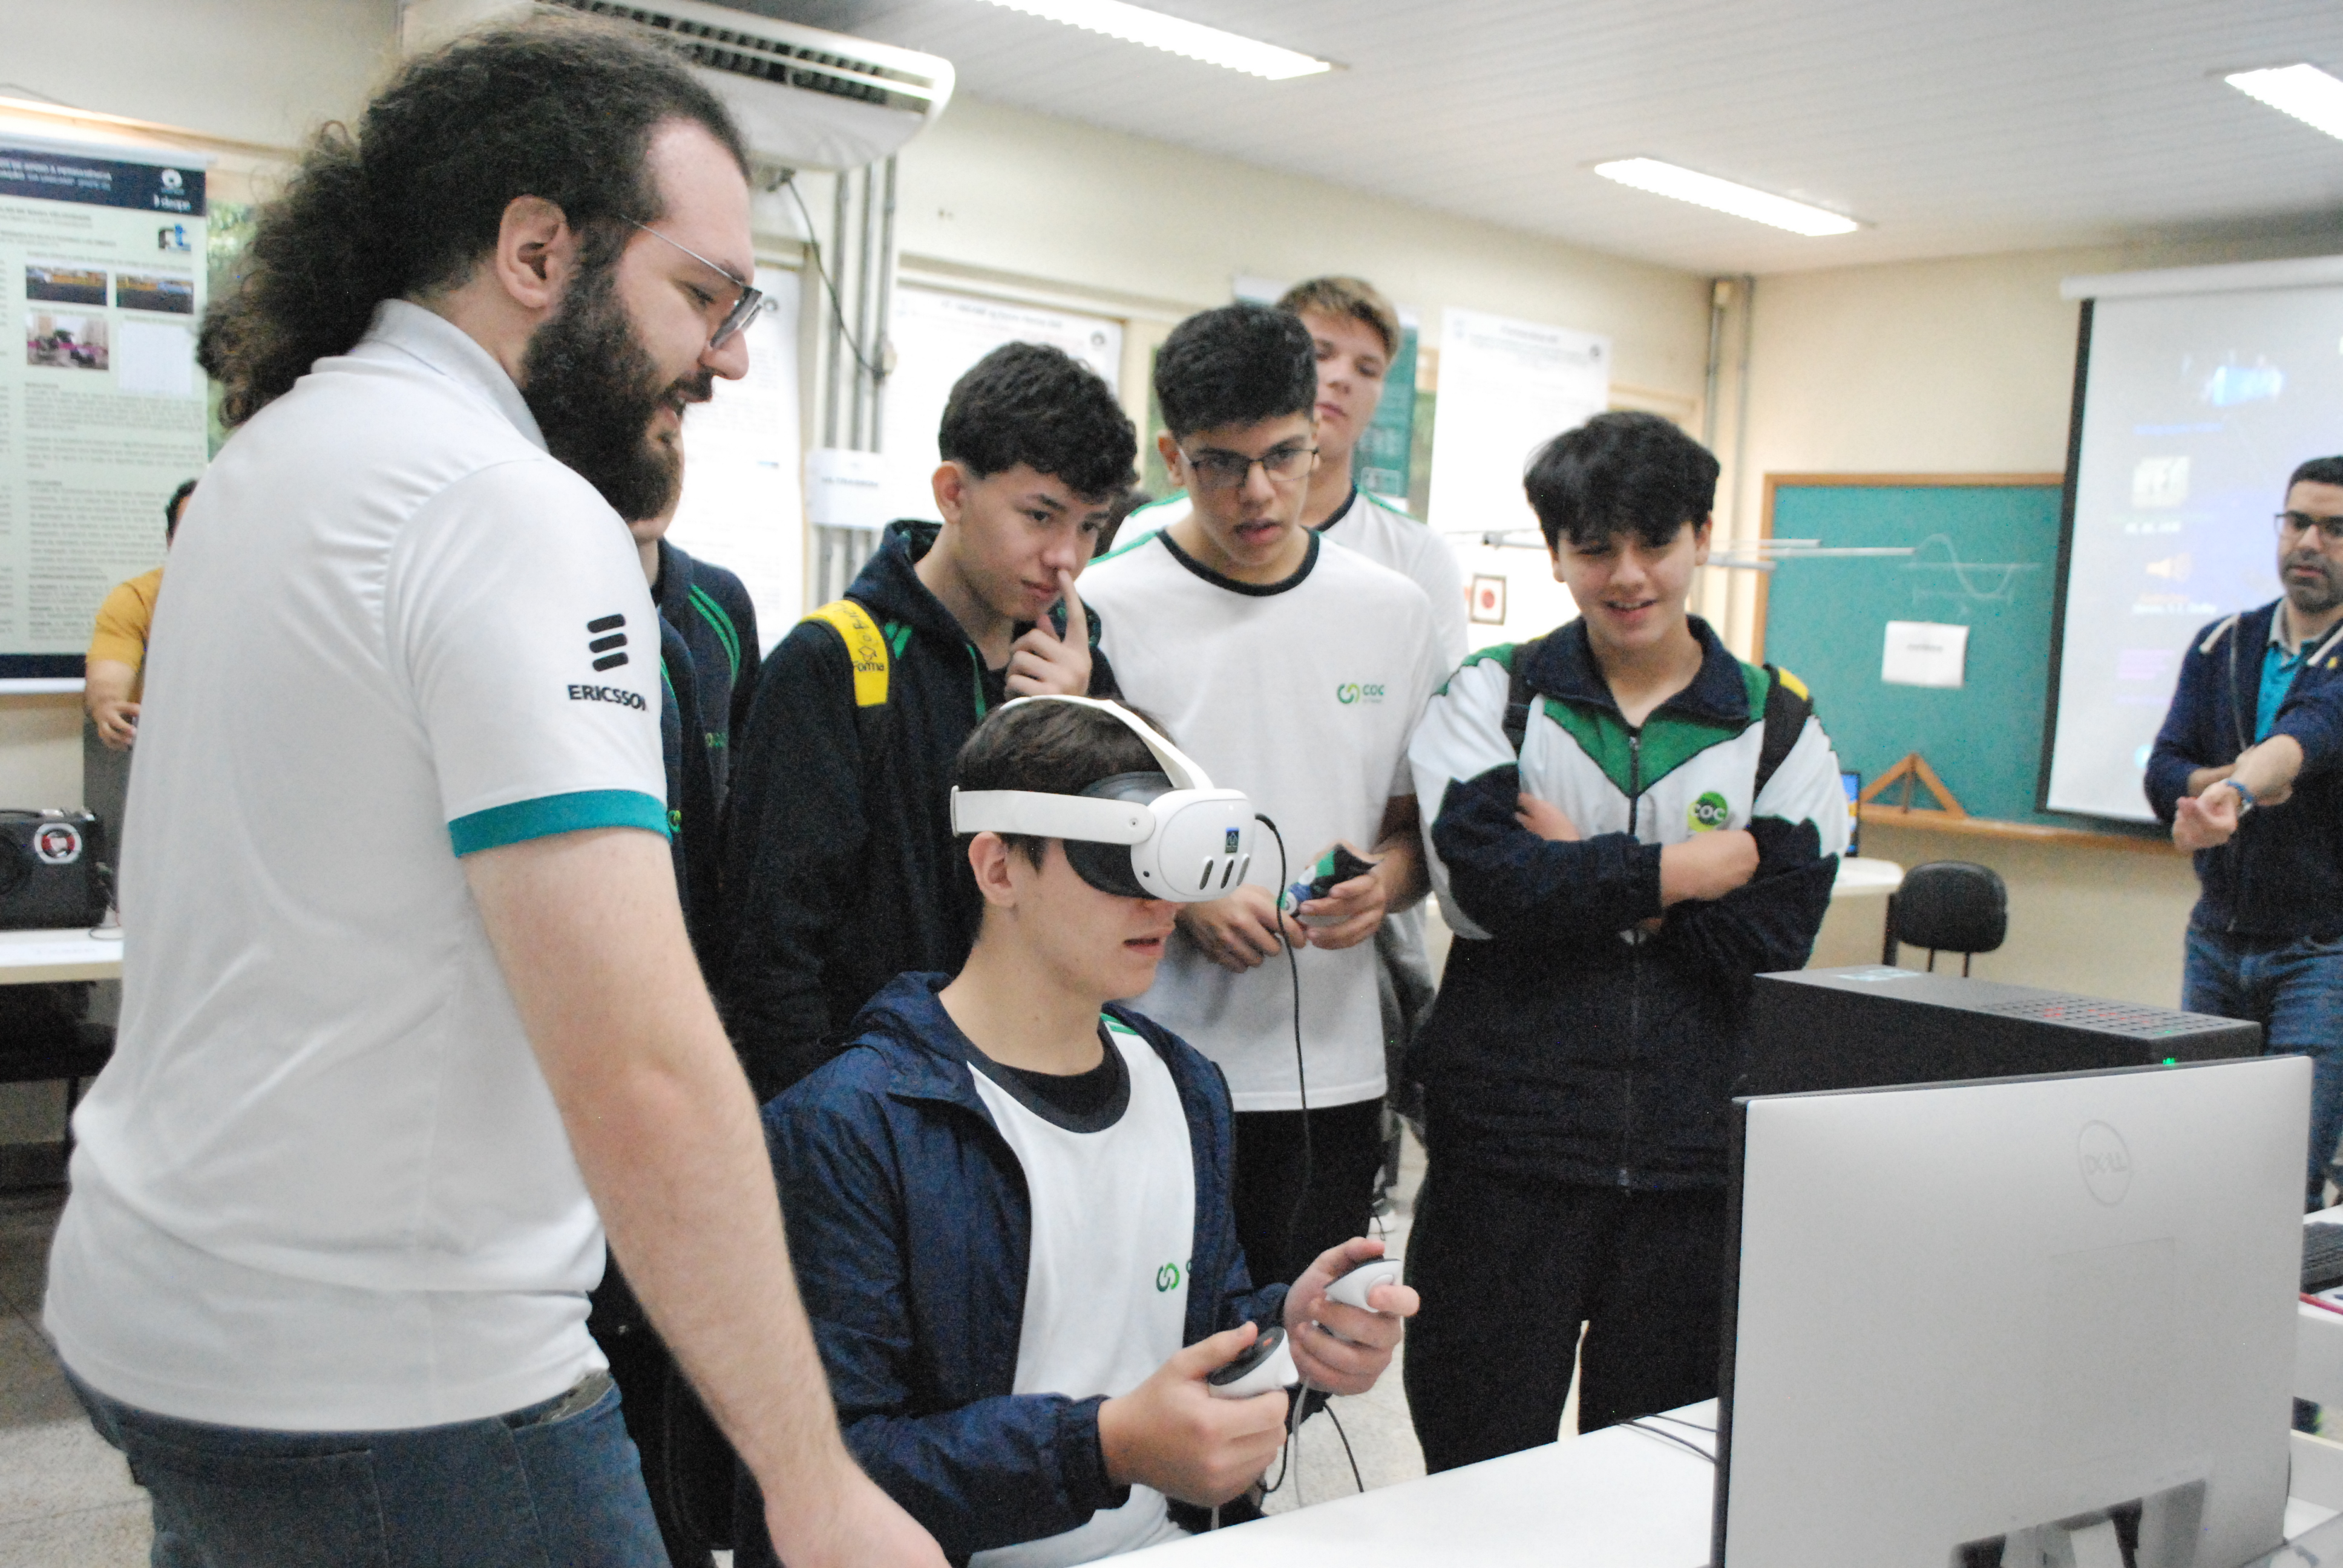
\includegraphics[width=0.8\linewidth,height=\textheight,keepaspectratio]{planejamento/dinamica-telecom.jpg}

}

\caption{Dinâmica da área de telecomunicações.}

\end{figure}%

As dinâmicas foram muito interativas e despertaram muito interesse nos
visitantes.

\begin{figure}[H]

{\centering 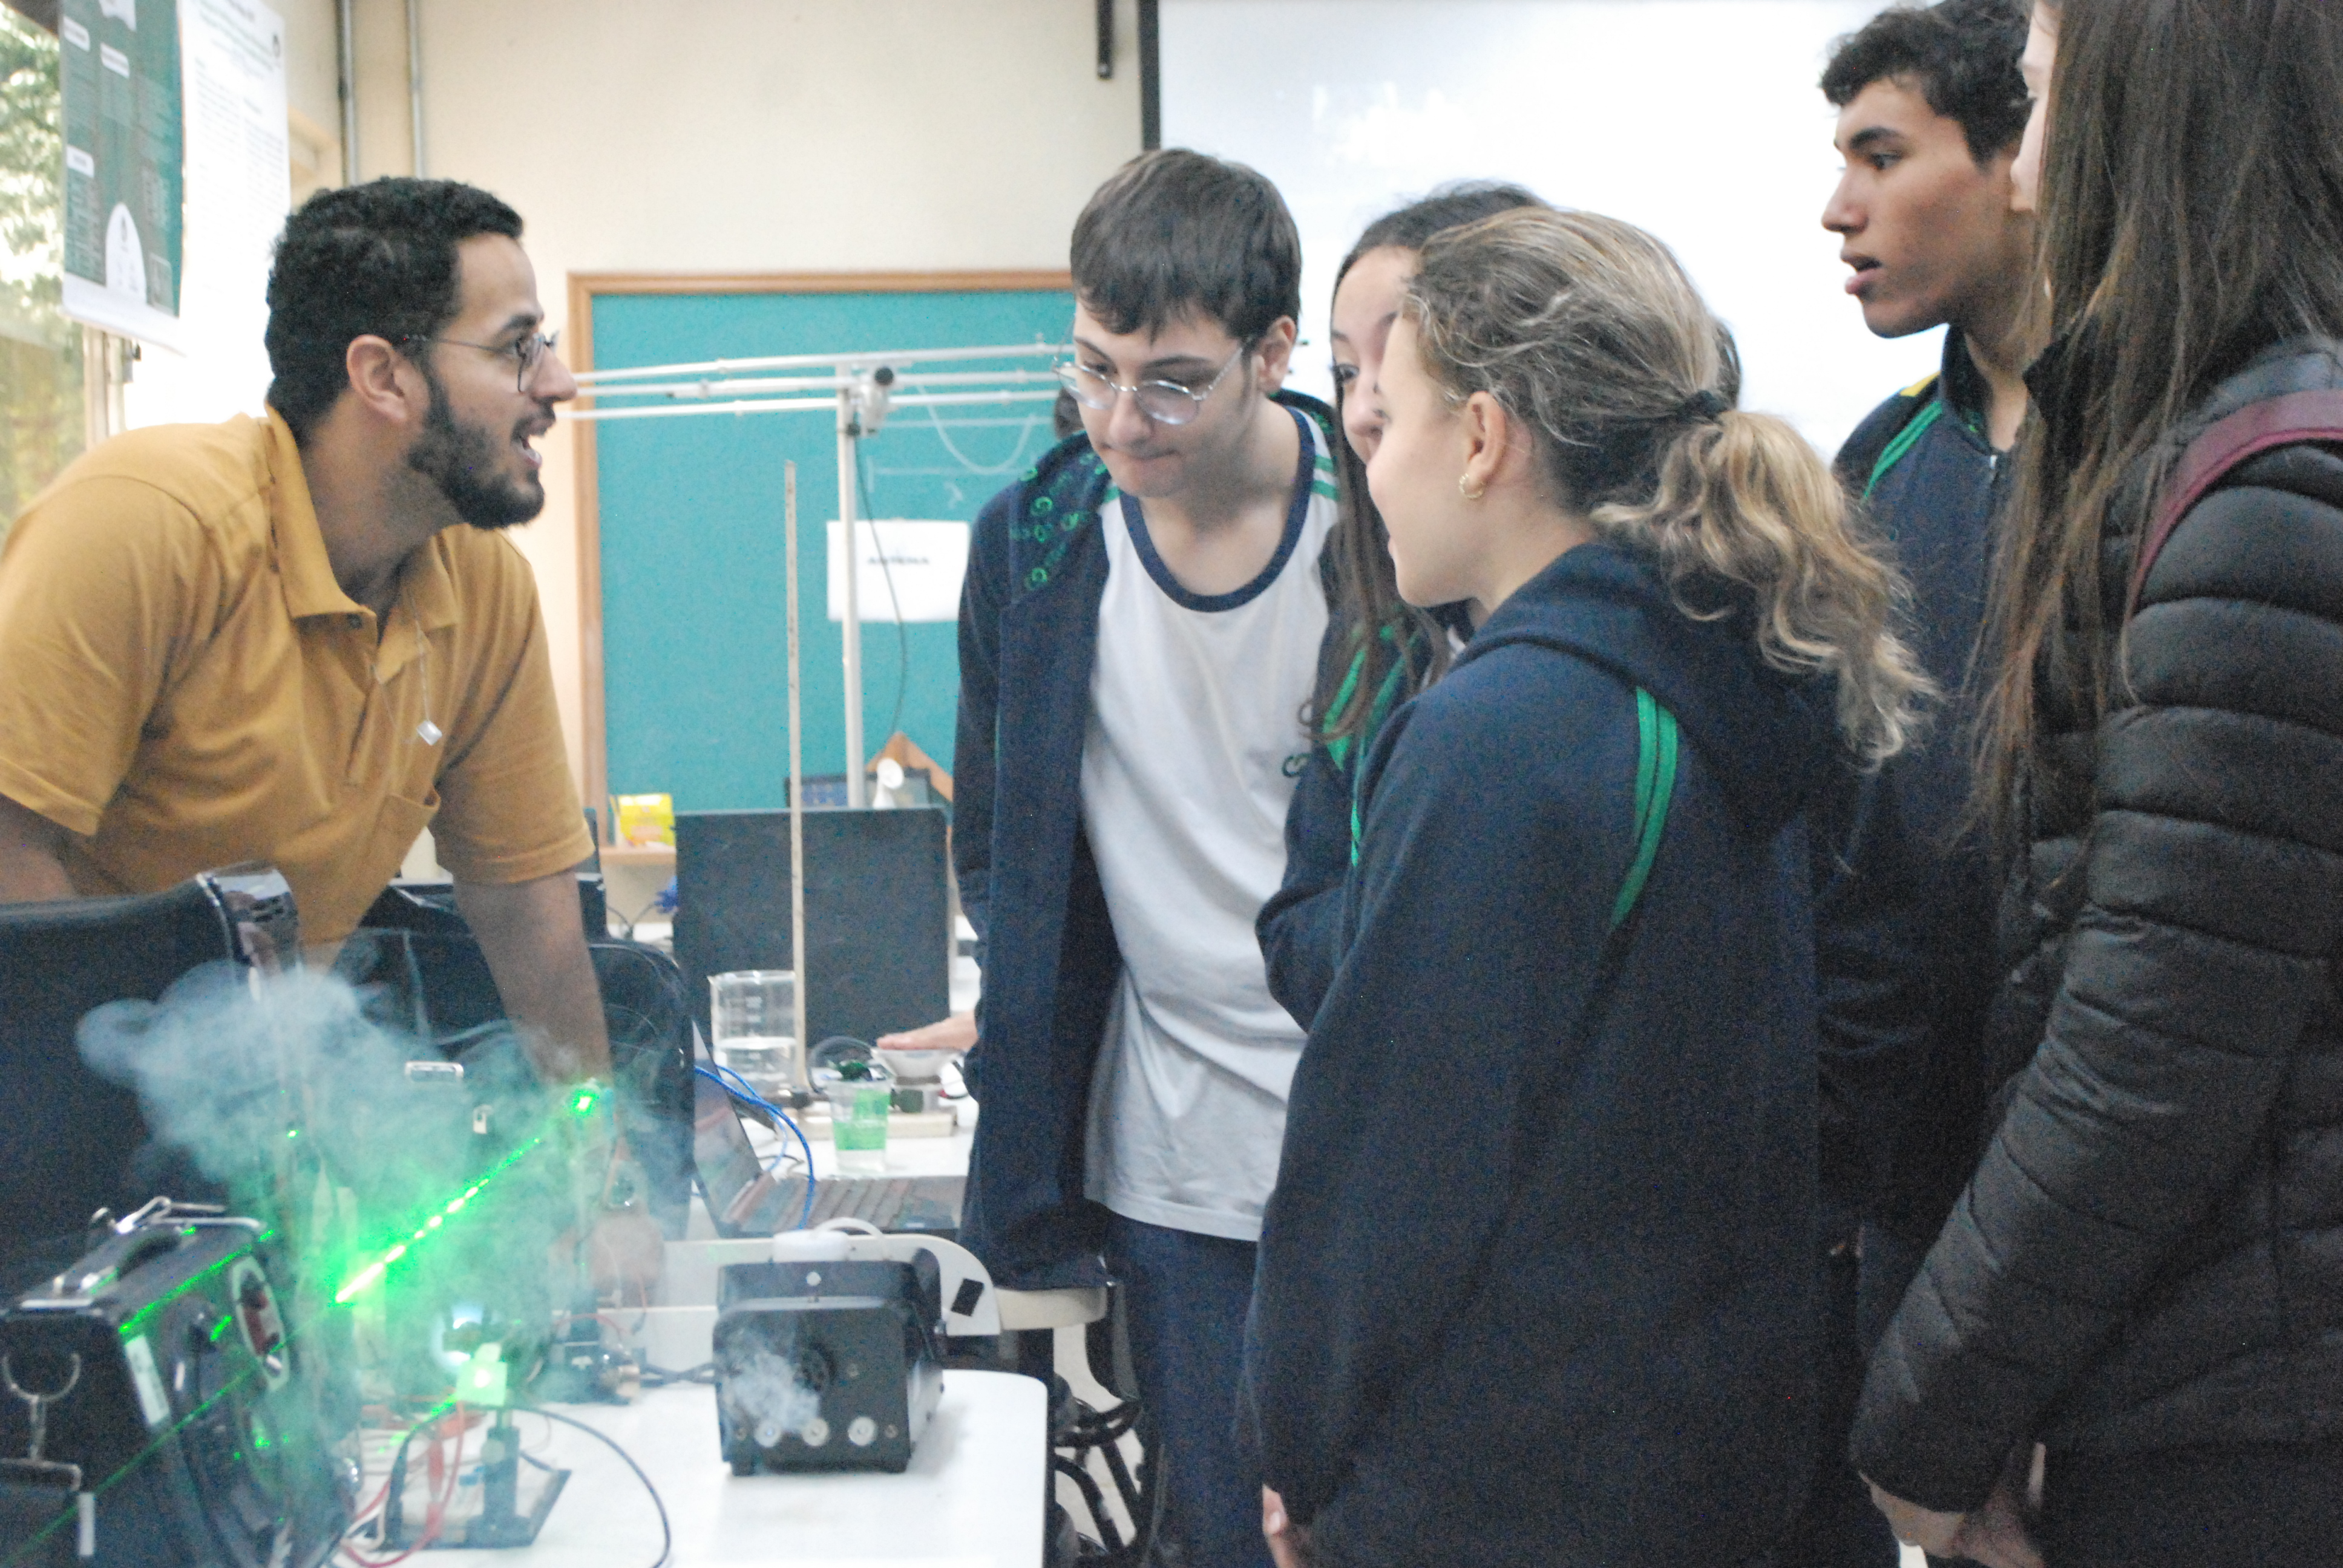
\includegraphics[width=0.6\linewidth,height=\textheight,keepaspectratio]{planejamento/exemplo-atividade-telecom-1.jpg}

}

\caption{Visitantes no FT de Portas Abertas assistindo demonstração de
transmissão de som usando laser.}

\end{figure}%

\begin{figure}[H]

{\centering 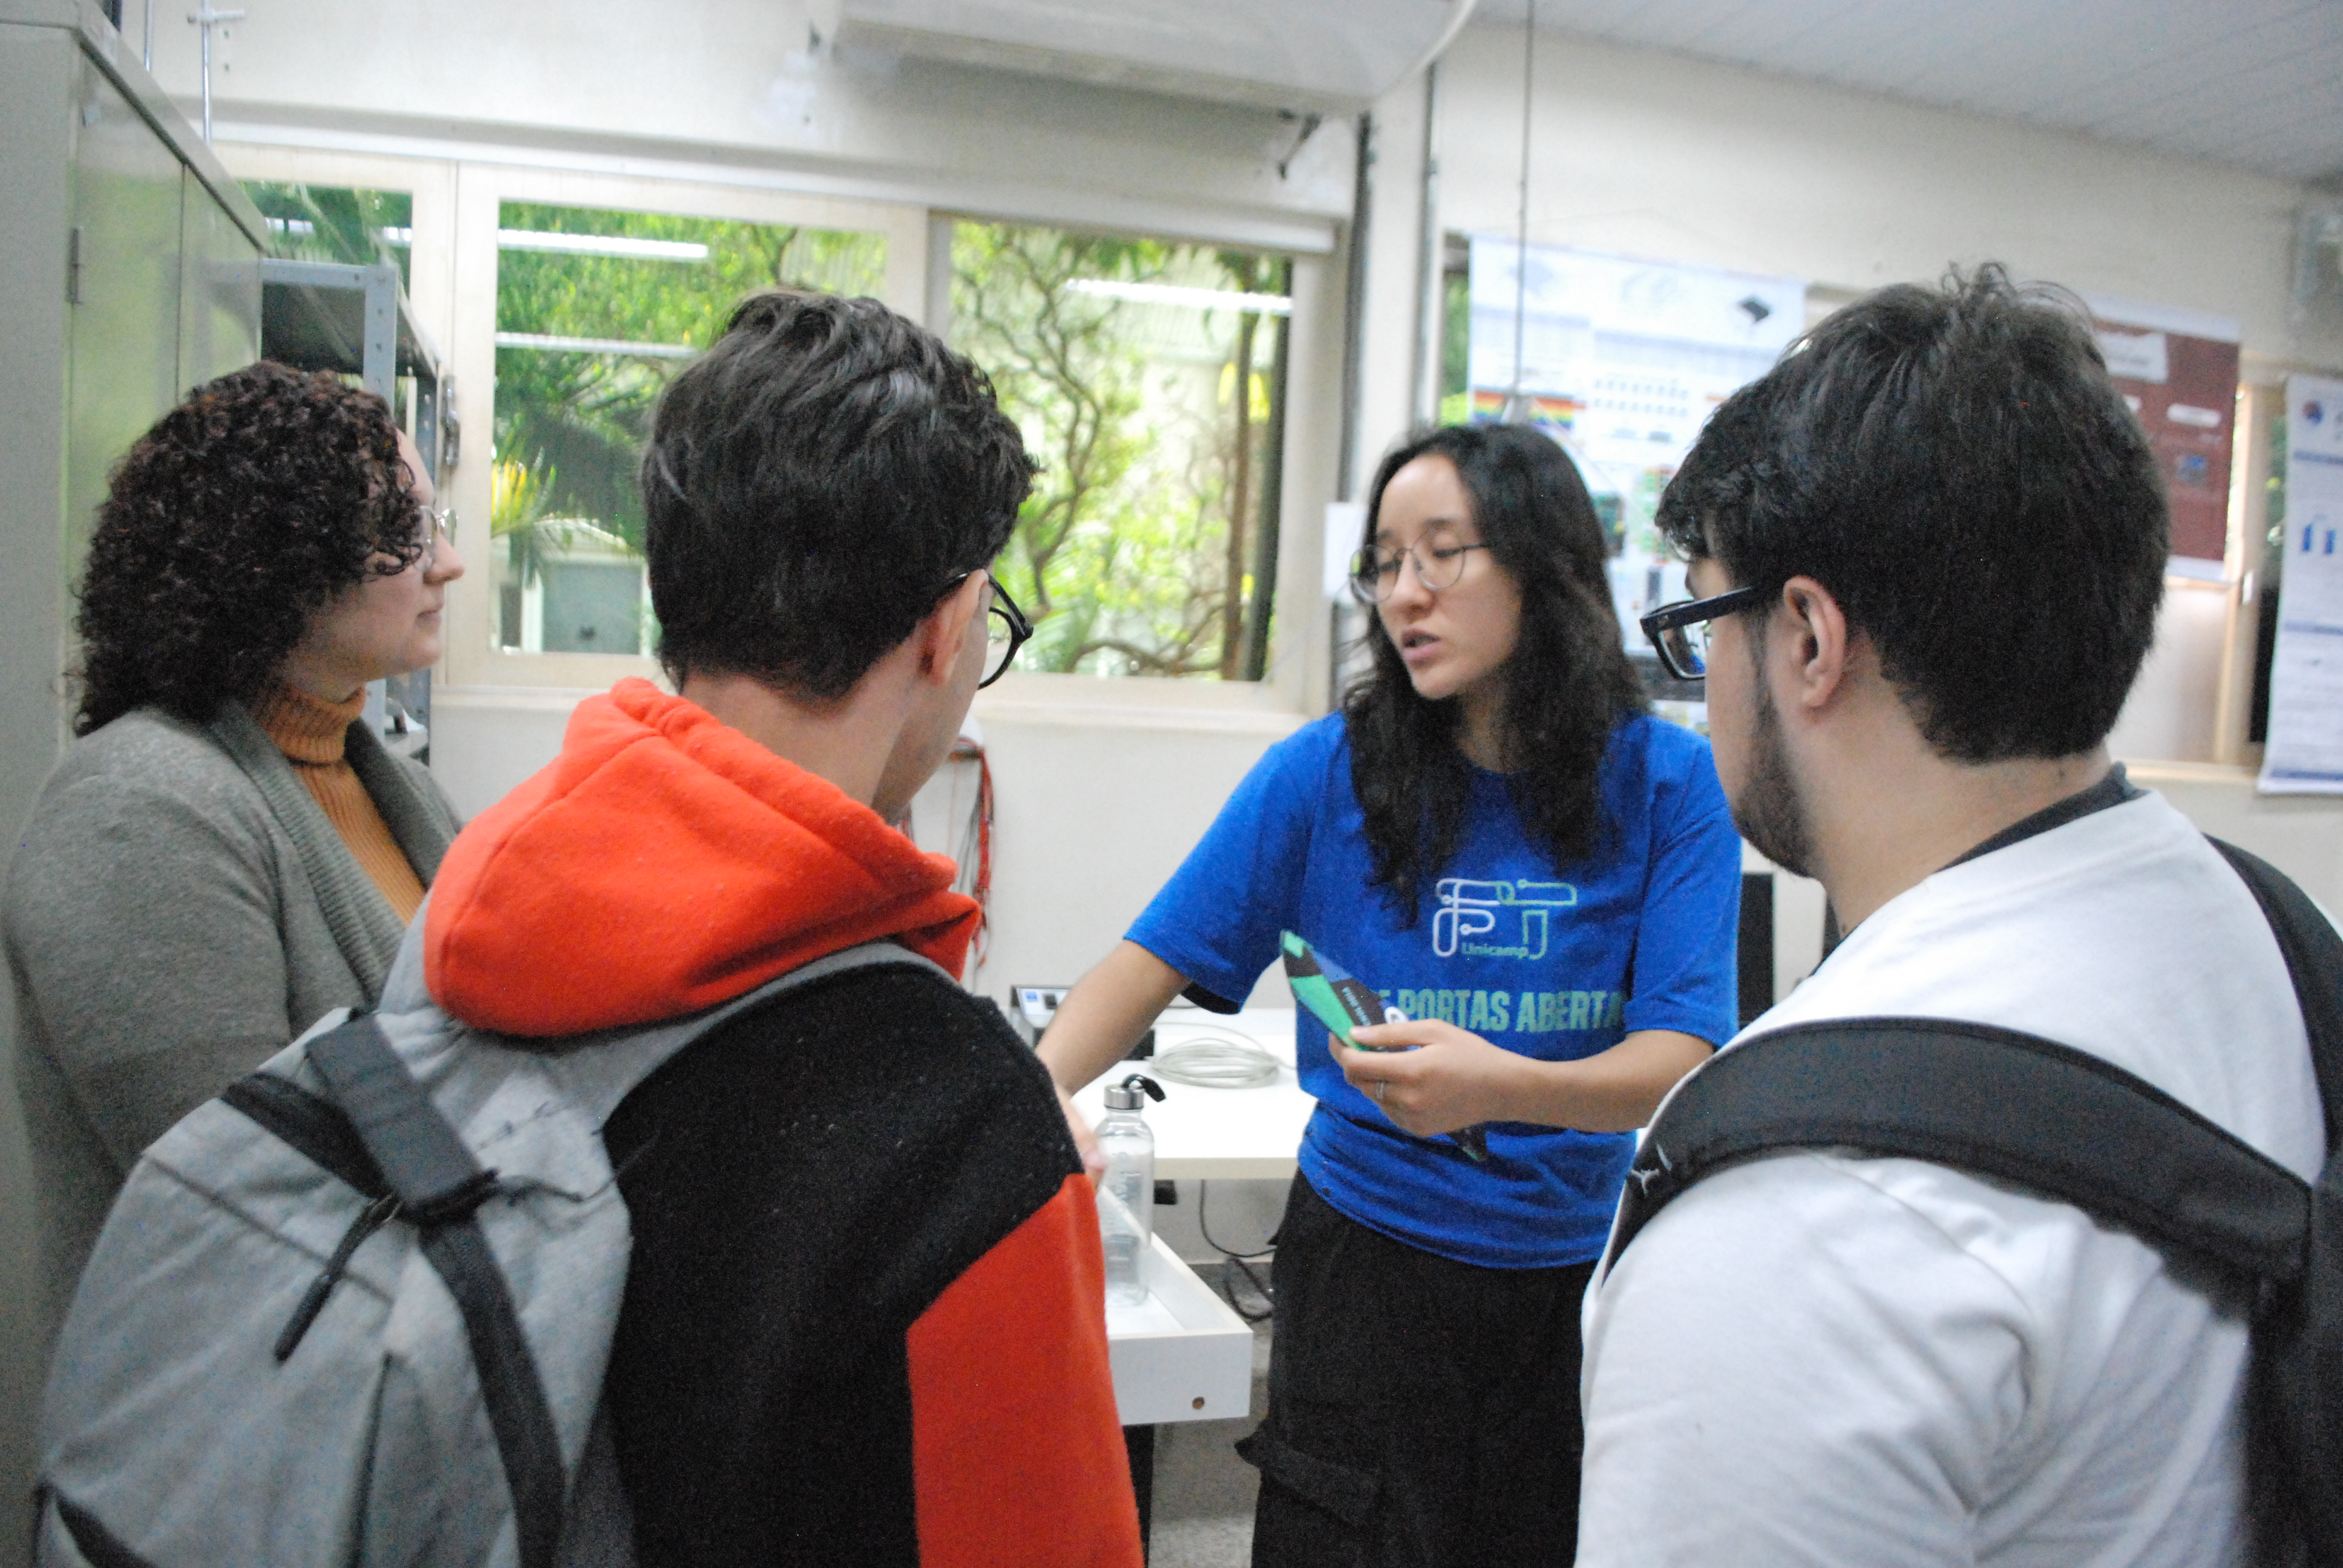
\includegraphics[width=0.6\linewidth,height=\textheight,keepaspectratio]{planejamento/exemplo-telecom-2.jpg}

}

\caption{Monitora explicando demonstração.}

\end{figure}%

O vídeo a seguir mostra a visitação no laboratório de Telecomunicações.

\url{video-telecom.mov}

Guiados por monitores, os visitantes eram levados para essas dinâmicas
por meio de uma trilha ilustrada na figura a seguir.

\begin{figure}[H]

{\centering \includegraphics[width=0.6\linewidth,height=\textheight,keepaspectratio]{planejamento/percurso-trilhas.png}

}

\caption{Representação esquemática em planta da FT, contendo o sentido
do percurso dos visitantes. As setas contínuas em preto, cinza (percurso
da Computação), verde (percurso Eng. de Transportes), azul (percurso
Eng. Ambiental), vermelho (percurso Eng. de Telecomunicações) e amarelo
(percurso final) indicam a trilha. O nome dos prédios principais e do
estacionamento estão identificados em cor branca e tarja preta.}

\end{figure}%

\section{Atrações}\label{atrauxe7uxf5es}

Além das dinâmicas, diversas atrações (atividades) foram realizadas:

\begin{itemize}
\tightlist
\item
  \emph{FT em Realidade Virtual}: A atividade mostrou nosso campus aos
  vistantes por meio de uma maquete virtual. O aplicativo em realidade
  virtual foi desenvolvido pelo doutorando Jhasmani Tito Cruz. O
  aplicativo usou dados coletados por drone e fornecidos pelo
  Prof.~Vitor Molina.
\end{itemize}

\includegraphics[width=0.6\linewidth,height=\textheight,keepaspectratio]{planejamento/maquete-virtual-1.jpg}
\includegraphics[width=0.6\linewidth,height=\textheight,keepaspectratio]{planejamento/maquete-virtual-2.jpg}
\includegraphics[width=0.6\linewidth,height=\textheight,keepaspectratio]{planejamento/maquete-virtual-3.jpg}

\begin{figure}[H]

{\centering \includegraphics[width=0.8\linewidth,height=\textheight,keepaspectratio]{planejamento/RV-2.jpeg}

}

\caption{Visitantes participando da atividade com realidade virtual.}

\end{figure}%

\begin{itemize}
\tightlist
\item
  \emph{Iniciação científica}: Trabalhos desenvolvidos por alunos da FT
  foram expostos no \href{https://explora.ft.unicamp.br/}{Explora}. Os
  vistantes puderam interagir com nossos alunos.
\end{itemize}

\begin{figure}[H]

{\centering \includegraphics[width=0.8\linewidth,height=\textheight,keepaspectratio]{planejamento/IC-1.jpeg}

}

\caption{Trabalho de TCC sobre controle de drone por gestos sendo
exposto para visitantes.}

\end{figure}%

\begin{itemize}
\item
  \emph{Onde estão os nossos formandos ?}: A atividade permitiu que os
  visitantes pudessem conversar com egressos da FT.
\item
  \emph{Organizações estudantis}: Algumas organizações estudantis da FT
  apresentaram seus projetos.
\end{itemize}

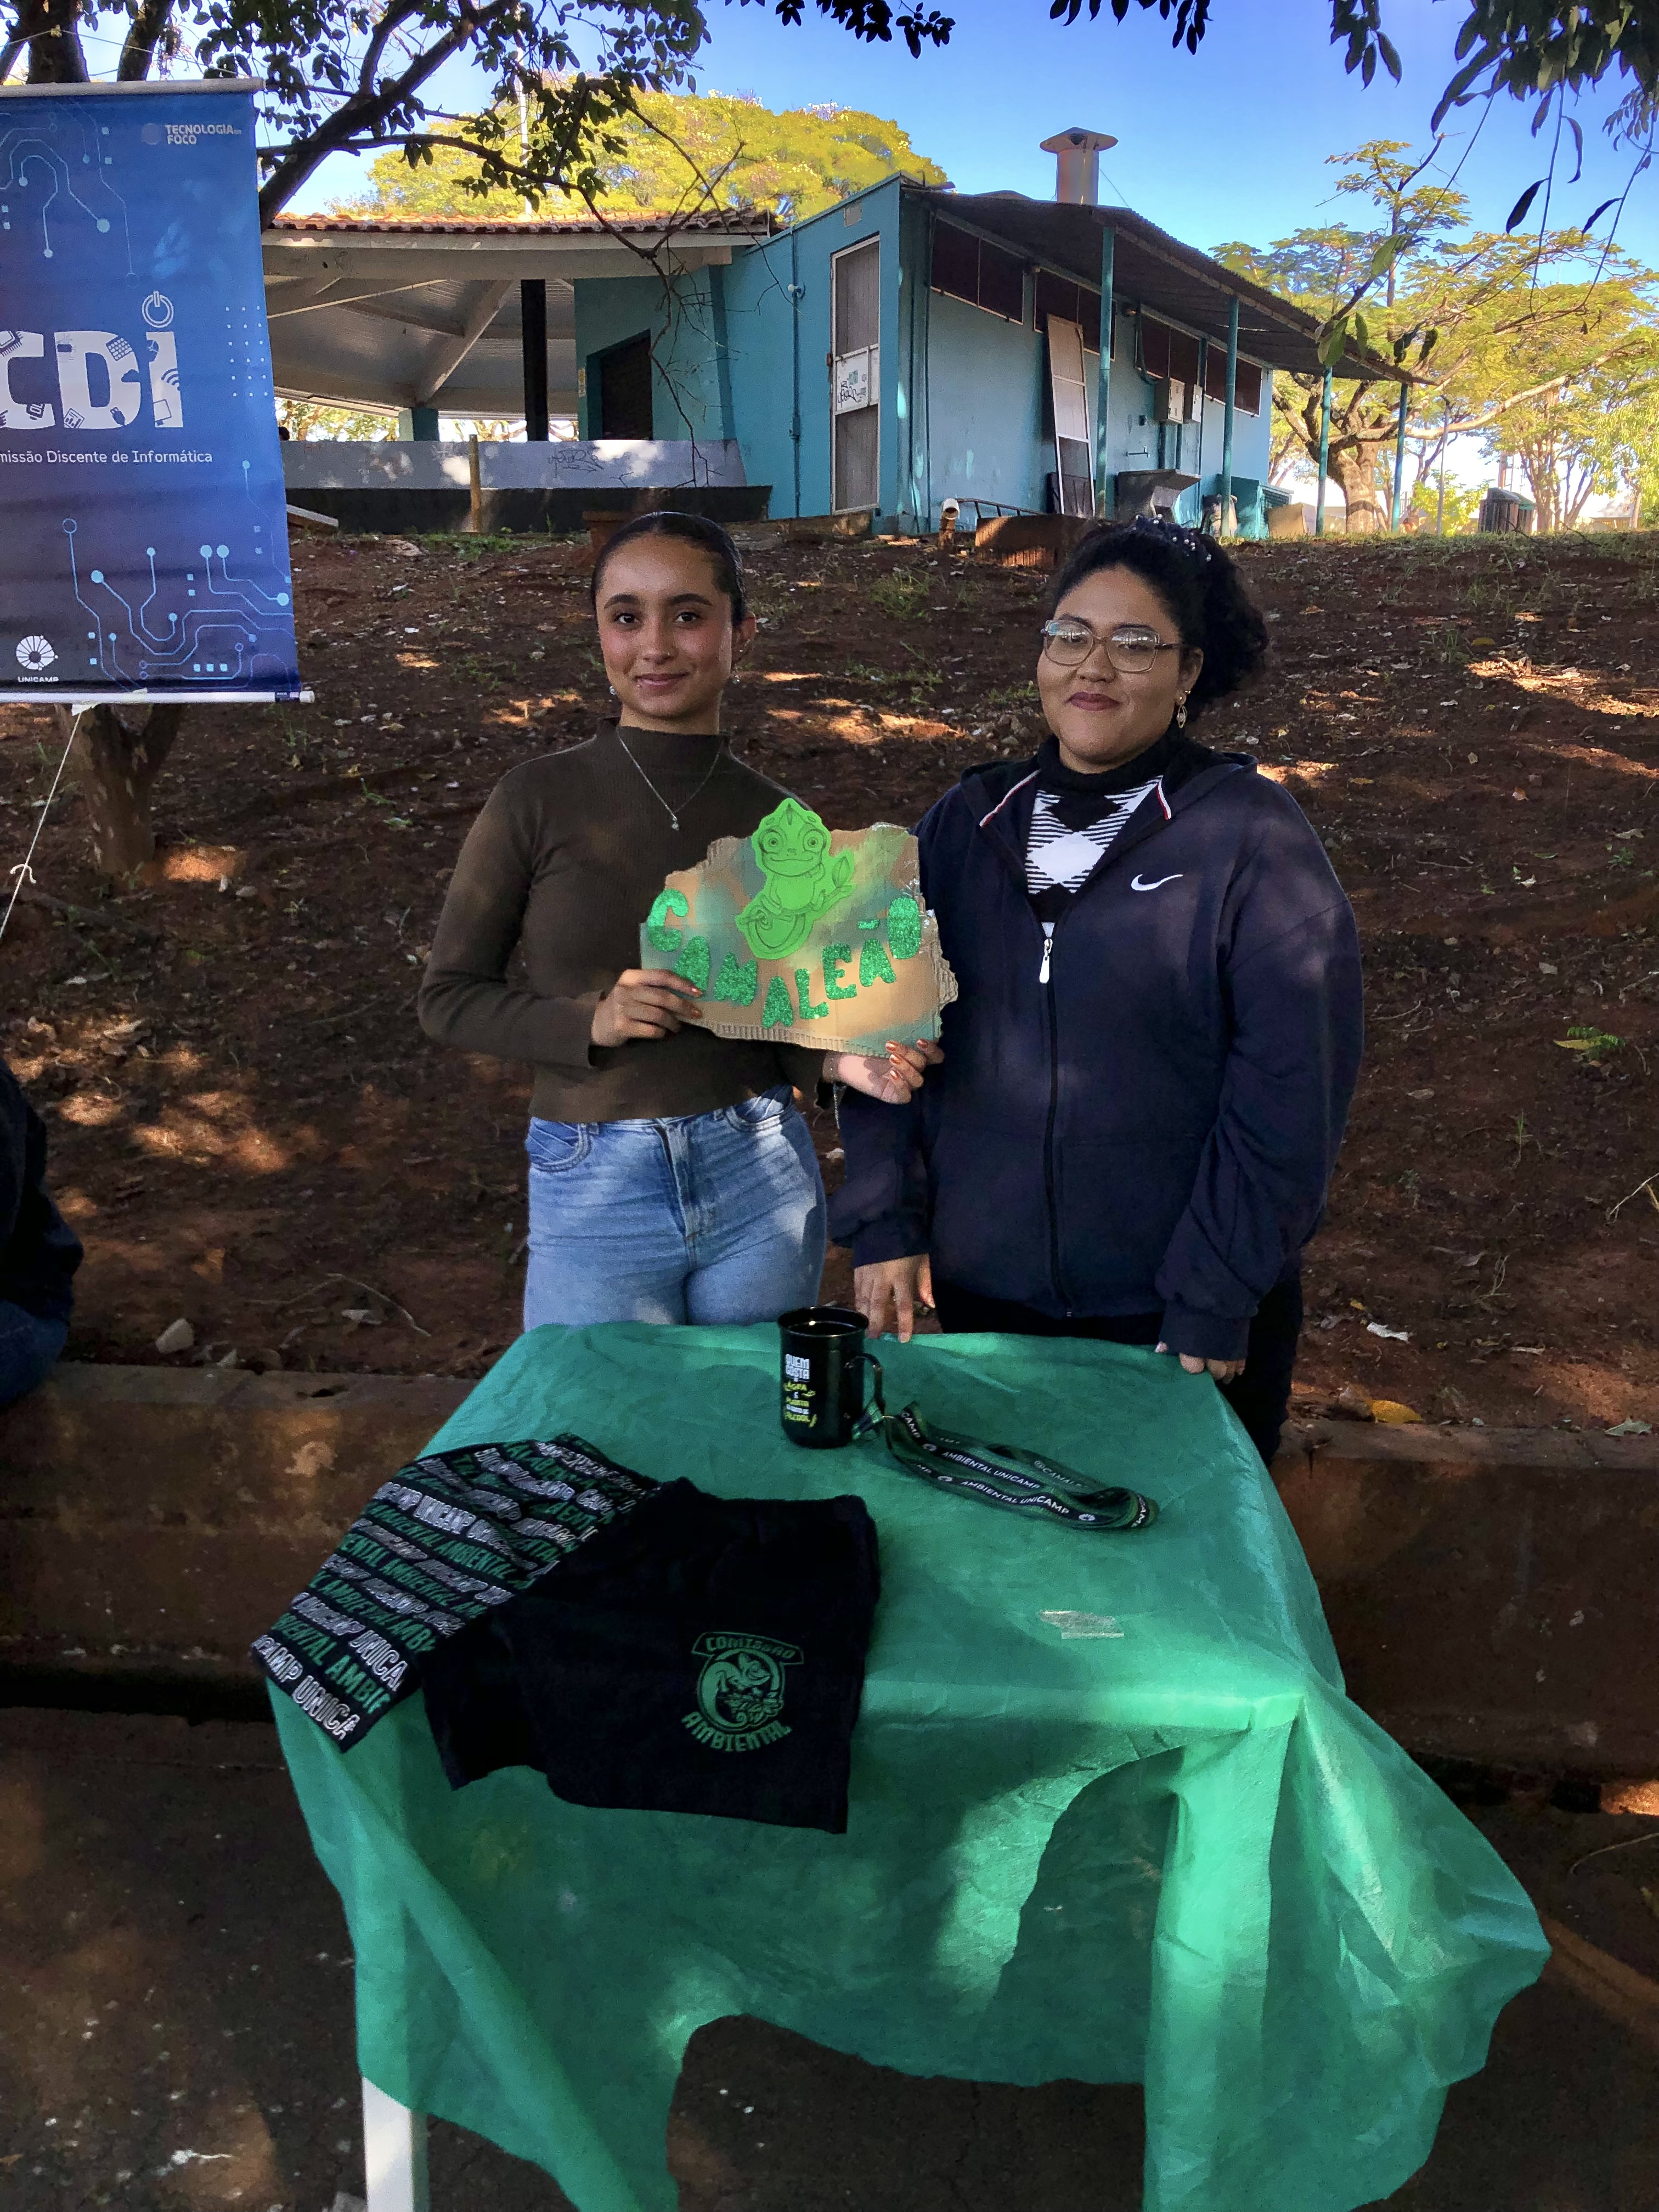
\includegraphics[width=0.4\linewidth,height=\textheight,keepaspectratio]{planejamento/org-est-1.jpg}
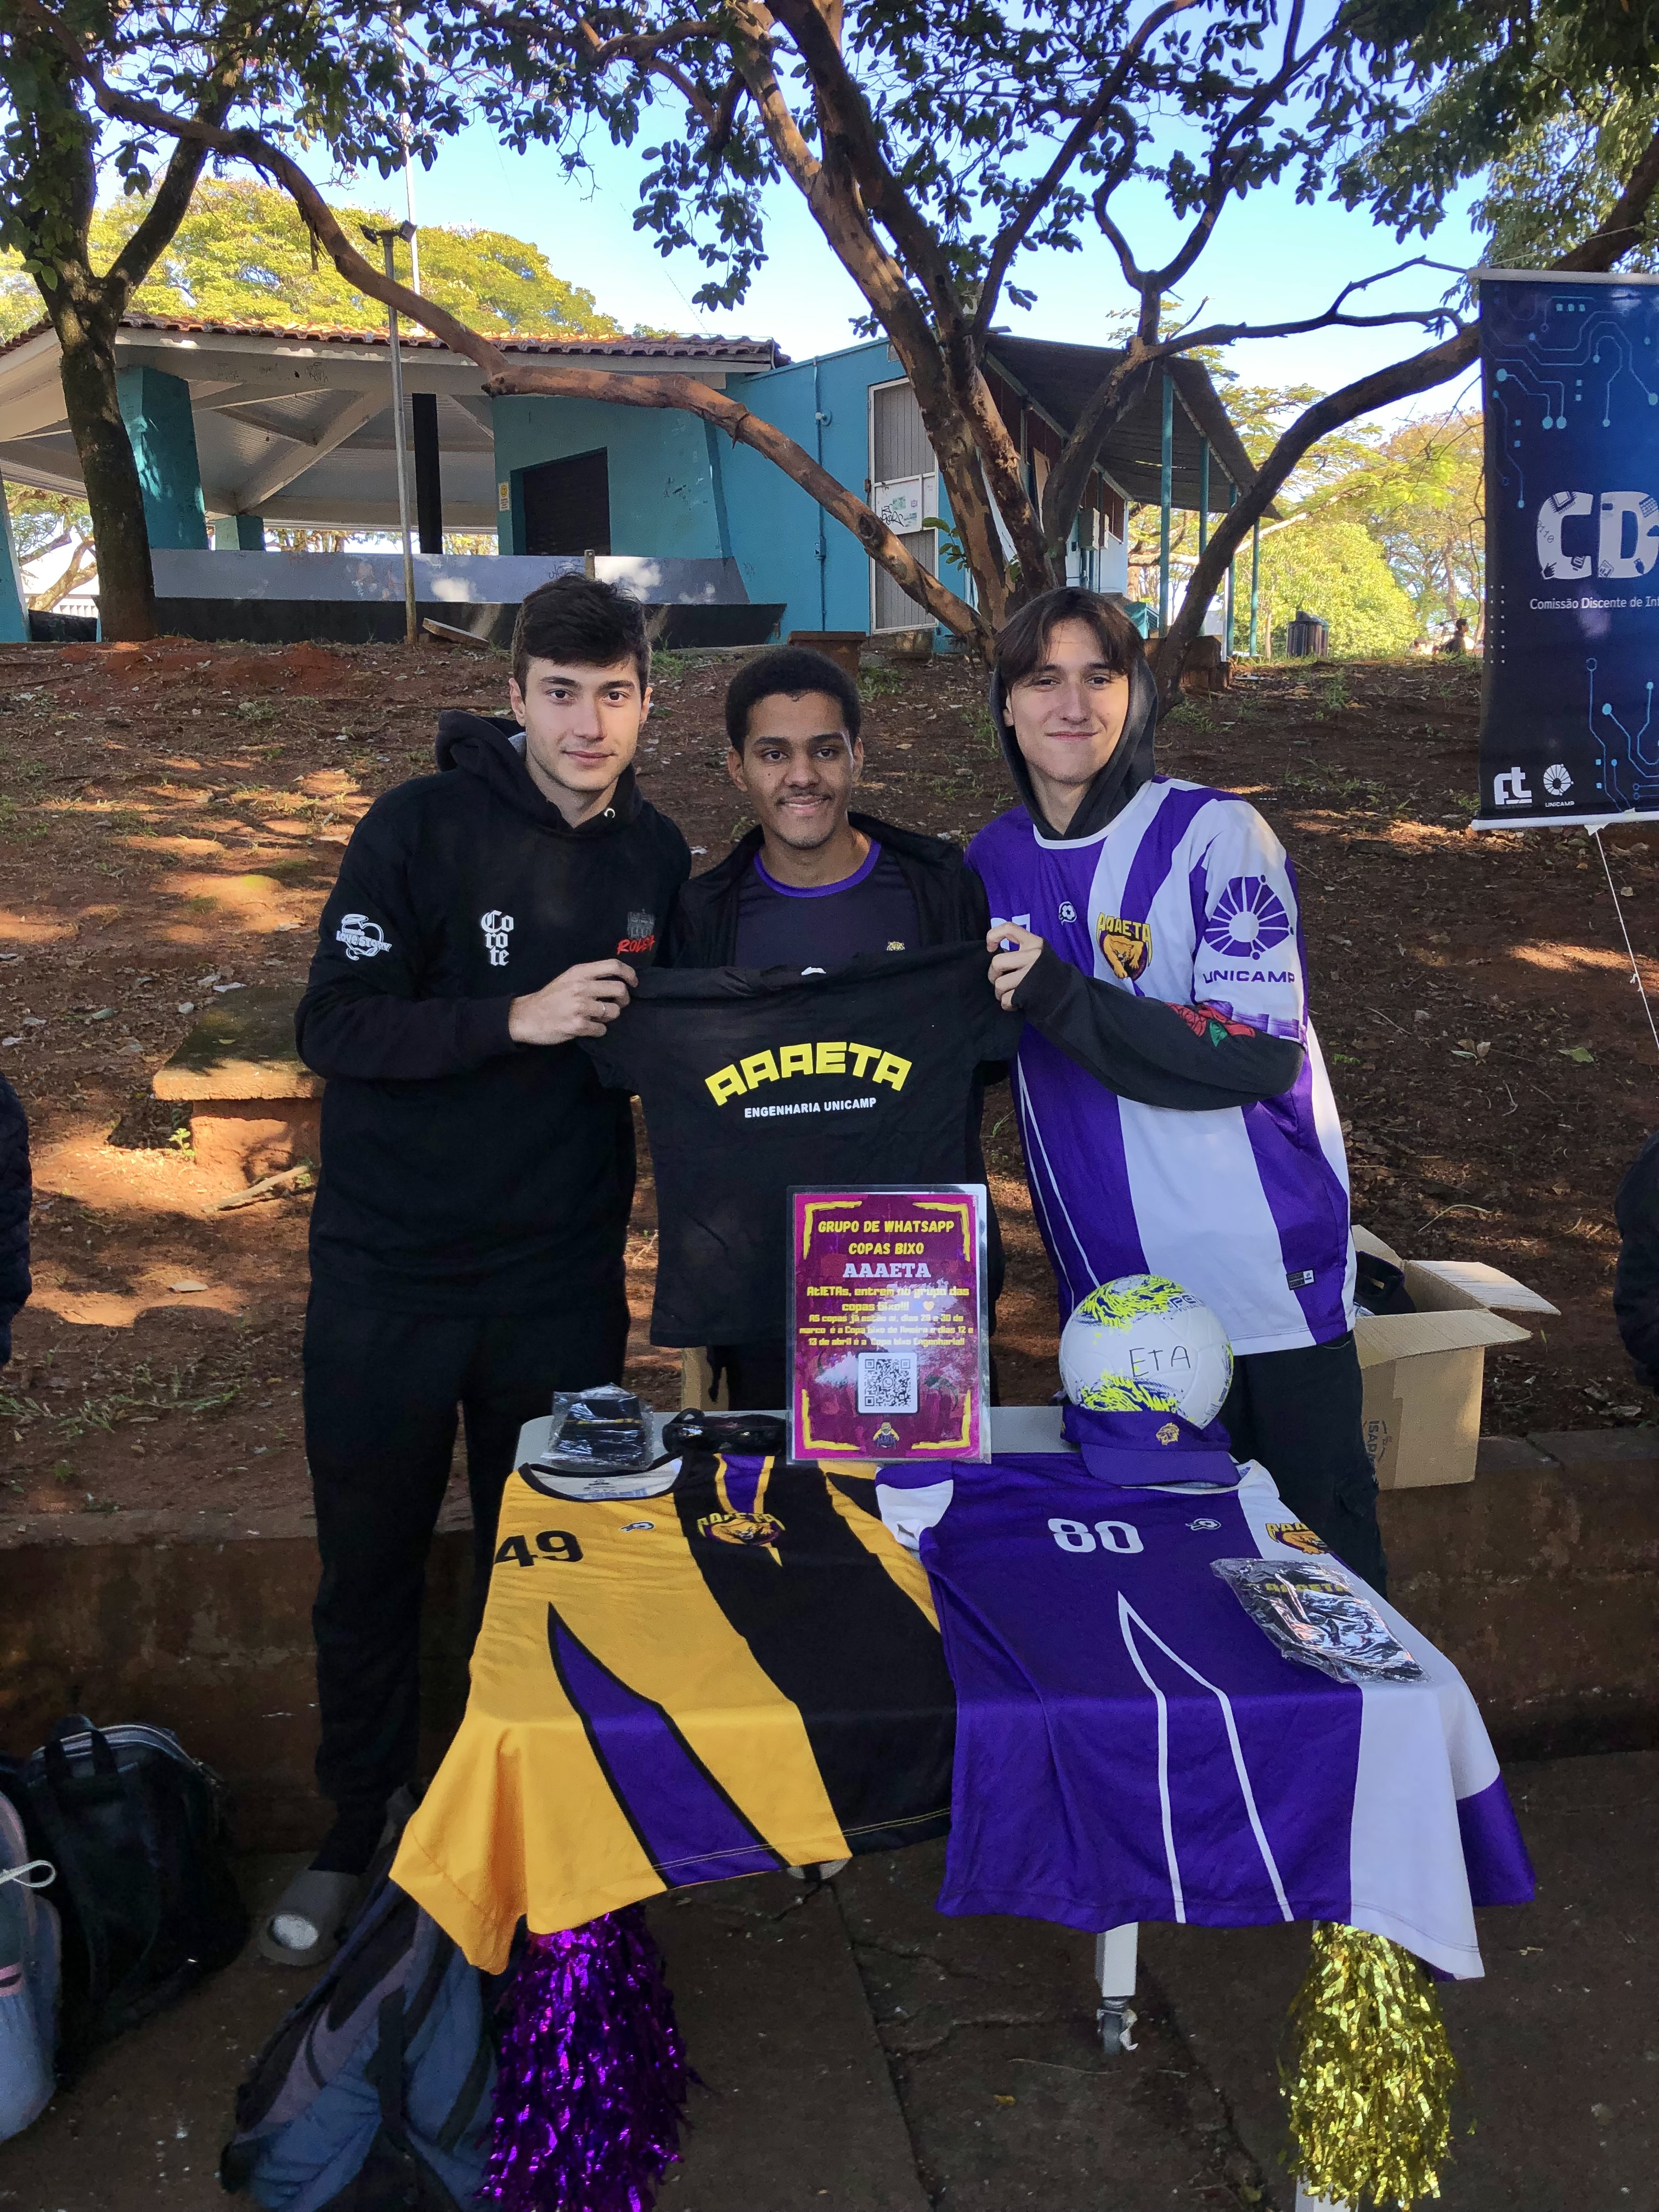
\includegraphics[width=0.4\linewidth,height=\textheight,keepaspectratio]{planejamento/org-est-2.jpg}
\includegraphics[width=0.4\linewidth,height=\textheight,keepaspectratio]{planejamento/org-est-3.jpg}
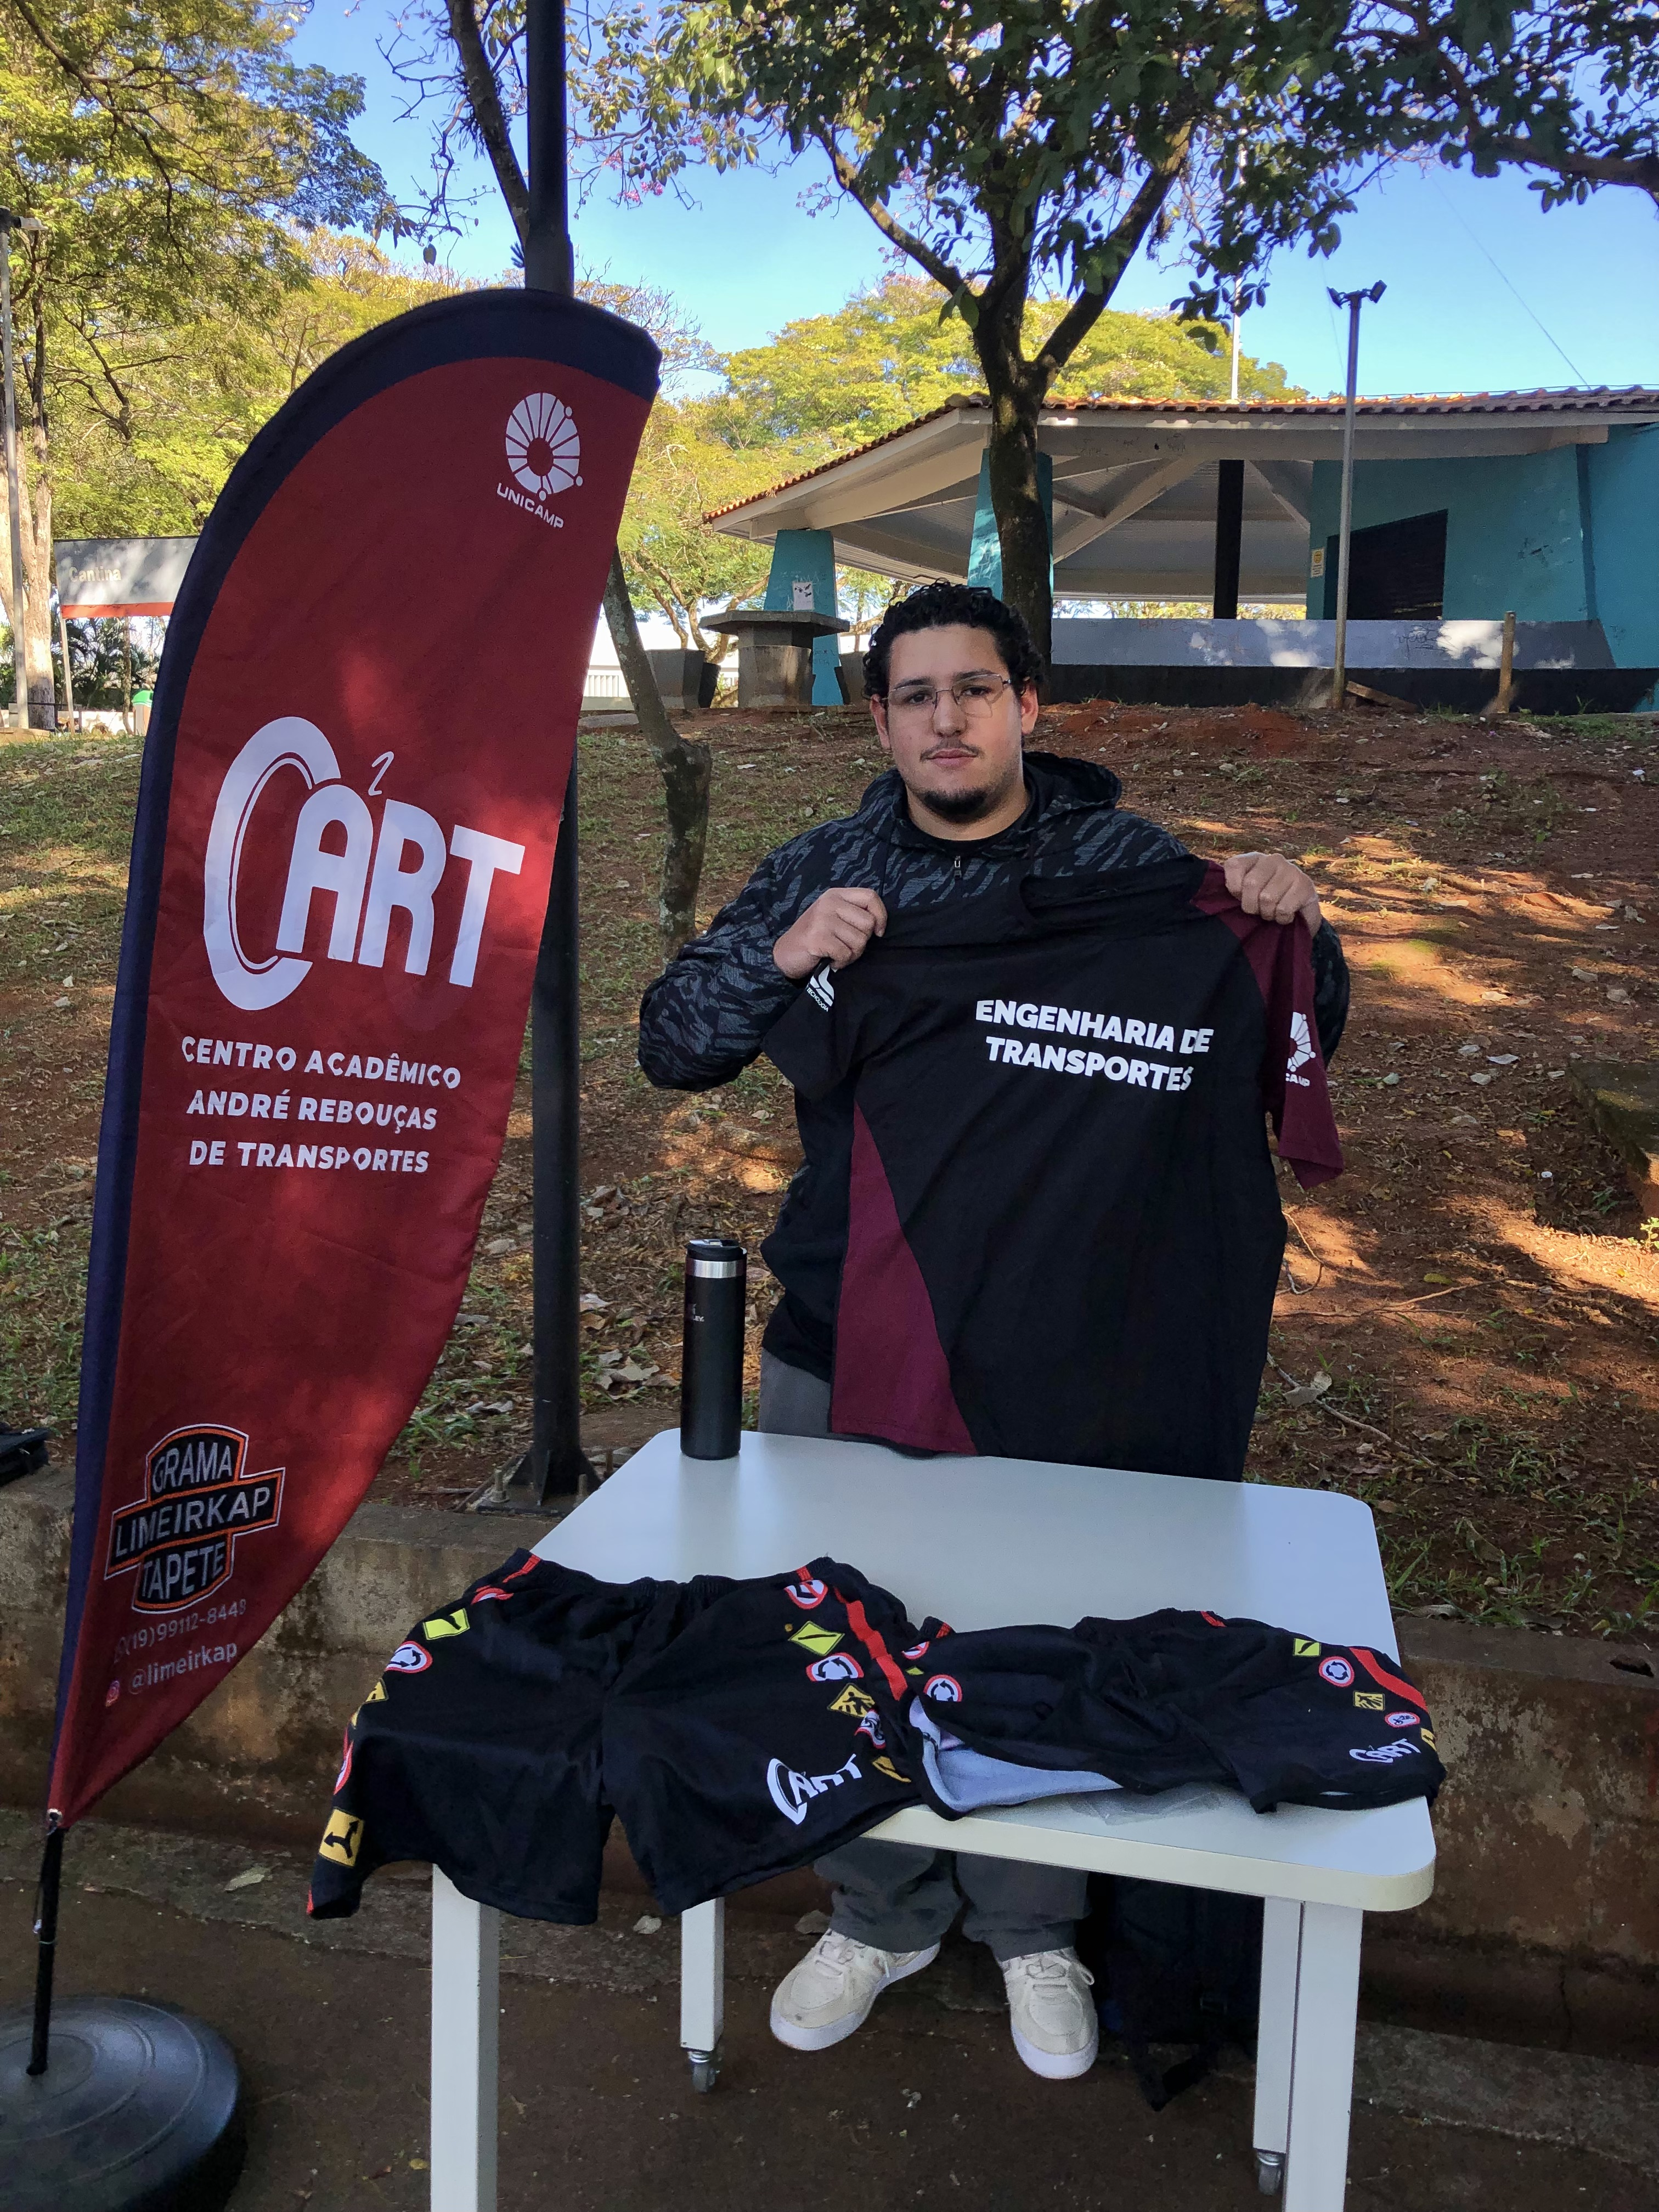
\includegraphics[width=0.4\linewidth,height=\textheight,keepaspectratio]{planejamento/org-est-4.jpg}
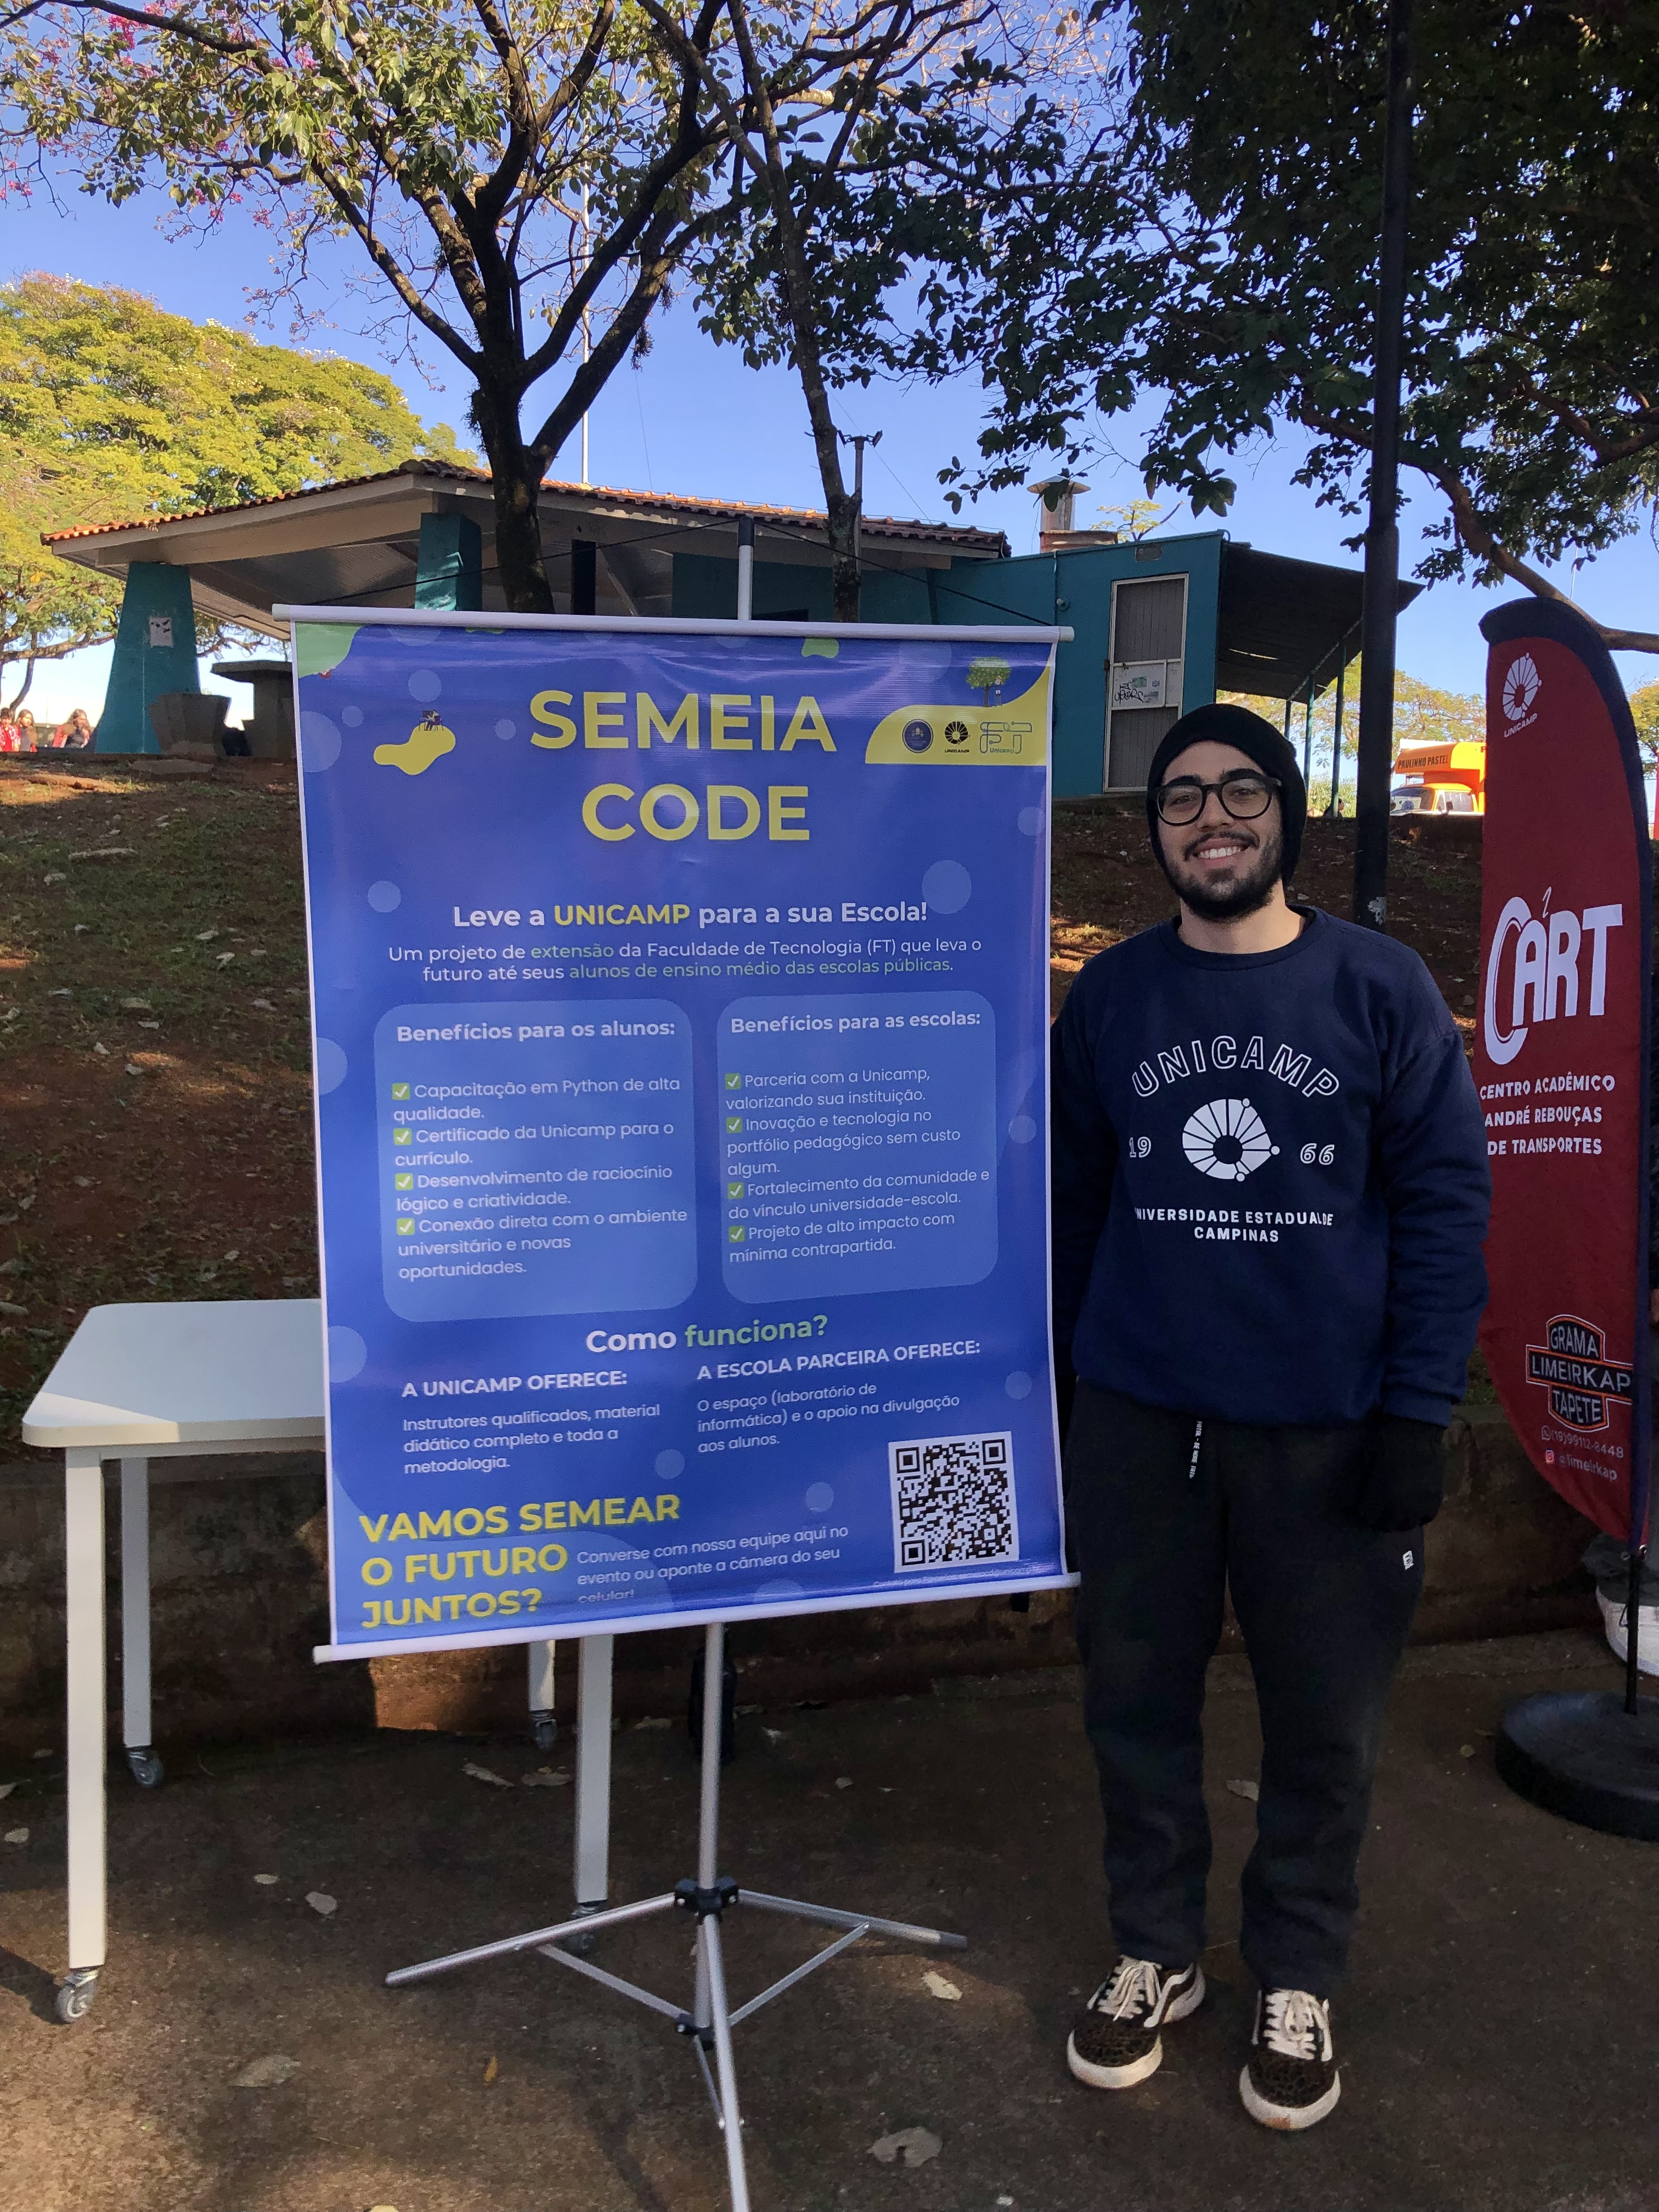
\includegraphics[width=0.4\linewidth,height=\textheight,keepaspectratio]{planejamento/org-est-5.jpg}
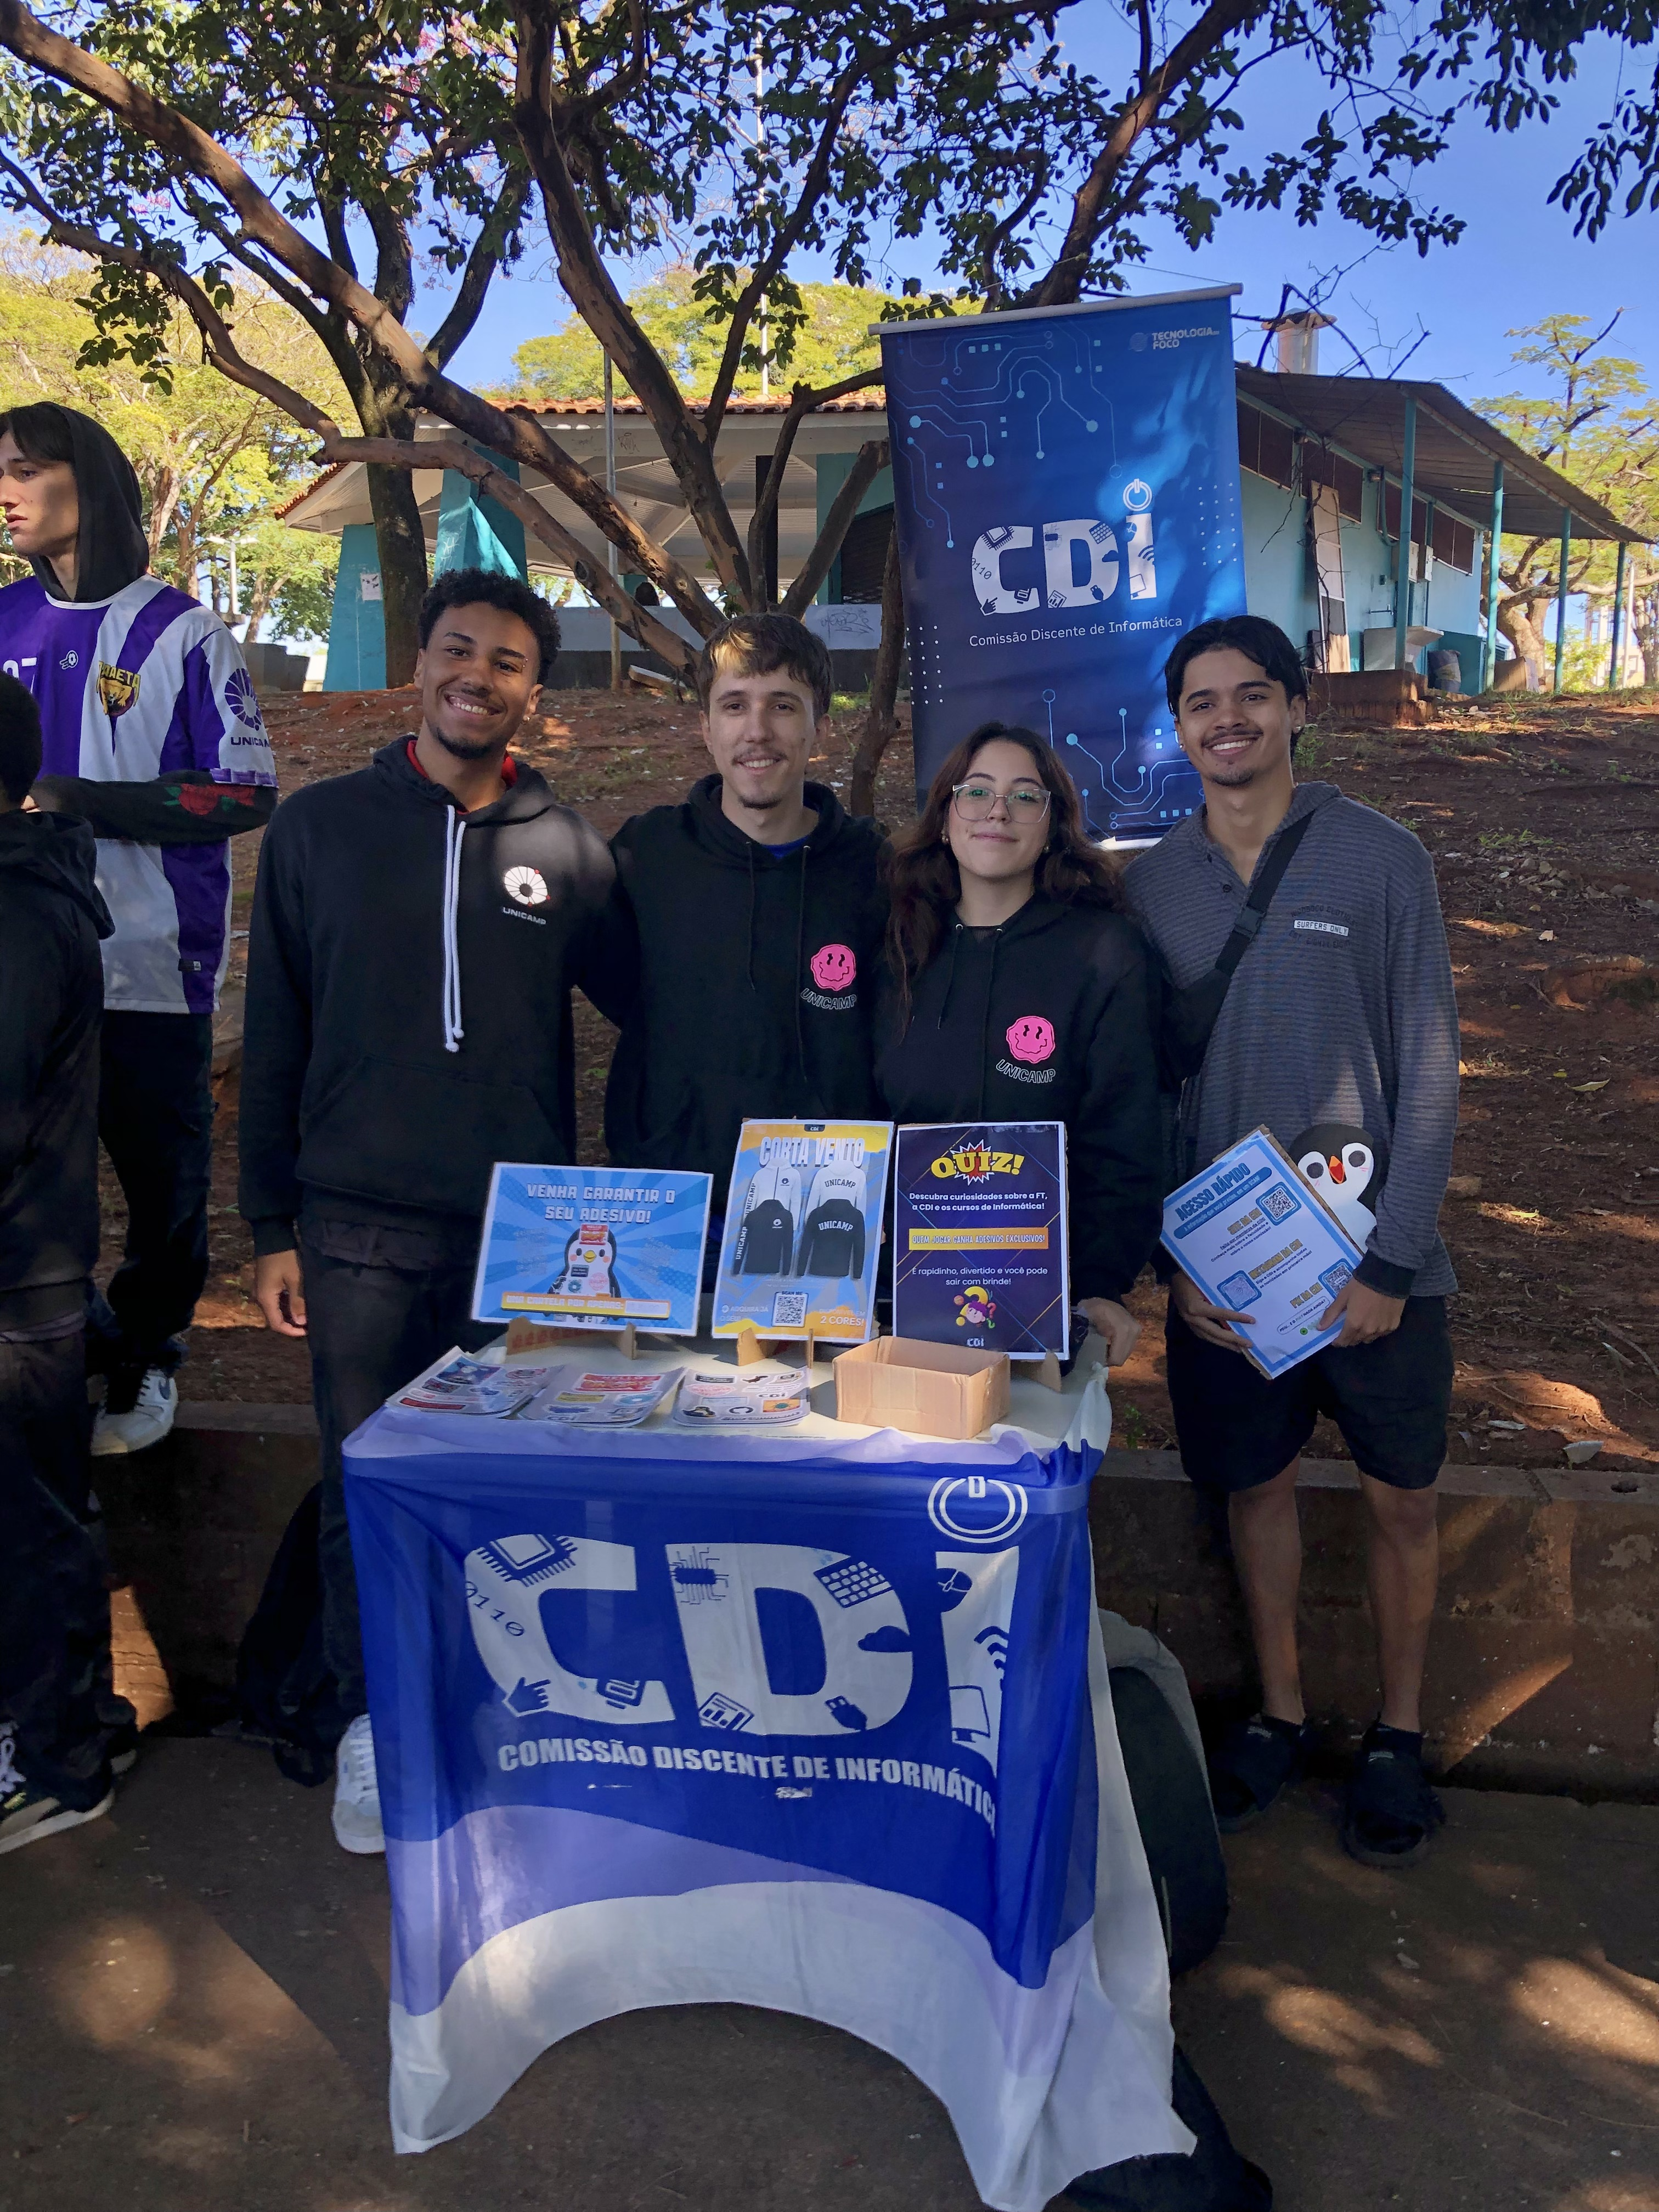
\includegraphics[width=0.4\linewidth,height=\textheight,keepaspectratio]{planejamento/org-est-6.jpg}

\begin{itemize}
\tightlist
\item
  \emph{Eu fui !}: A LP04 se transformou num estúdio de fotos onde os
  vistantes puderam registrar sua participação no evento. Após a foto,
  um email era encaminhado para o visitante contendo a foto tirada e a
  seguinte mensagem:
\end{itemize}

\begin{verbatim}
Olá !

Agradeçemos sua participação no evento FT de Portas Abertas !

Esperamos que a experiência tenha sido enriquecedora.

Em anexo, estamos enviando a foto de recordação do evento.

Mais informações sobre a Faculdade de Tecnologia/Unicamp
podem ser vistas em https://www.ft.unicamp.br/ .

Informações sobre o vestibular da Unicamp podem ser obtidas 
em https://www.comvest.unicamp.br/ .

Comissão organizadora.
\end{verbatim}

A seguir, podemos ver o mural das fotos tiradas no estúdio de fotos.

\begin{figure}[H]

{\centering \includegraphics[width=0.9\linewidth,height=\textheight,keepaspectratio]{planejamento/estudio-1.jpg}

}

\caption{Fotos com os visitantes.}

\end{figure}%

\begin{figure}[H]

{\centering \includegraphics[width=0.9\linewidth,height=\textheight,keepaspectratio]{planejamento/estudio-2.jpg}

}

\caption{Fotos com a equipe de organização.}

\end{figure}%

\begin{itemize}
\tightlist
\item
  \emph{Ecoedu Ambiental}: O projeto Ecoedu apresentou suas atividades,
  principalmente seu projeto de ensino de Libras.
\end{itemize}

\includegraphics[width=0.7\linewidth,height=\textheight,keepaspectratio]{planejamento/visita-ecoedu.jpg}

\begin{itemize}
\tightlist
\item
  \emph{Inova}: A agência Inova da Unicamp montou uma estande no FT de
  Portas Abertas e apresentou uma palestra para os visitantes,
  divulgando principalmente o evento ``Inova Jovem''.
\end{itemize}

\includegraphics[width=0.5\linewidth,height=\textheight,keepaspectratio]{planejamento/participacao-inova.jpg}
\includegraphics[width=0.8\linewidth,height=\textheight,keepaspectratio]{planejamento/palestra-inova.jpg}

A Inova publicou uma matéria sobre sua participação no FT de Portas
Abertas que pode ser vista
\href{https://www.inova.unicamp.br/2025/06/inova-unicamp-apresenta-programa-de-empreendedorismo-para-jovens-durante-o-ft-de-portas-abertas/}{aqui}.

\begin{itemize}
\tightlist
\item
  \emph{Equipe Unicamp Racing Team 1600}: A equipe da FT que compete na
  fórmula 1600 apresentou seu projeto durante o evento.
\end{itemize}

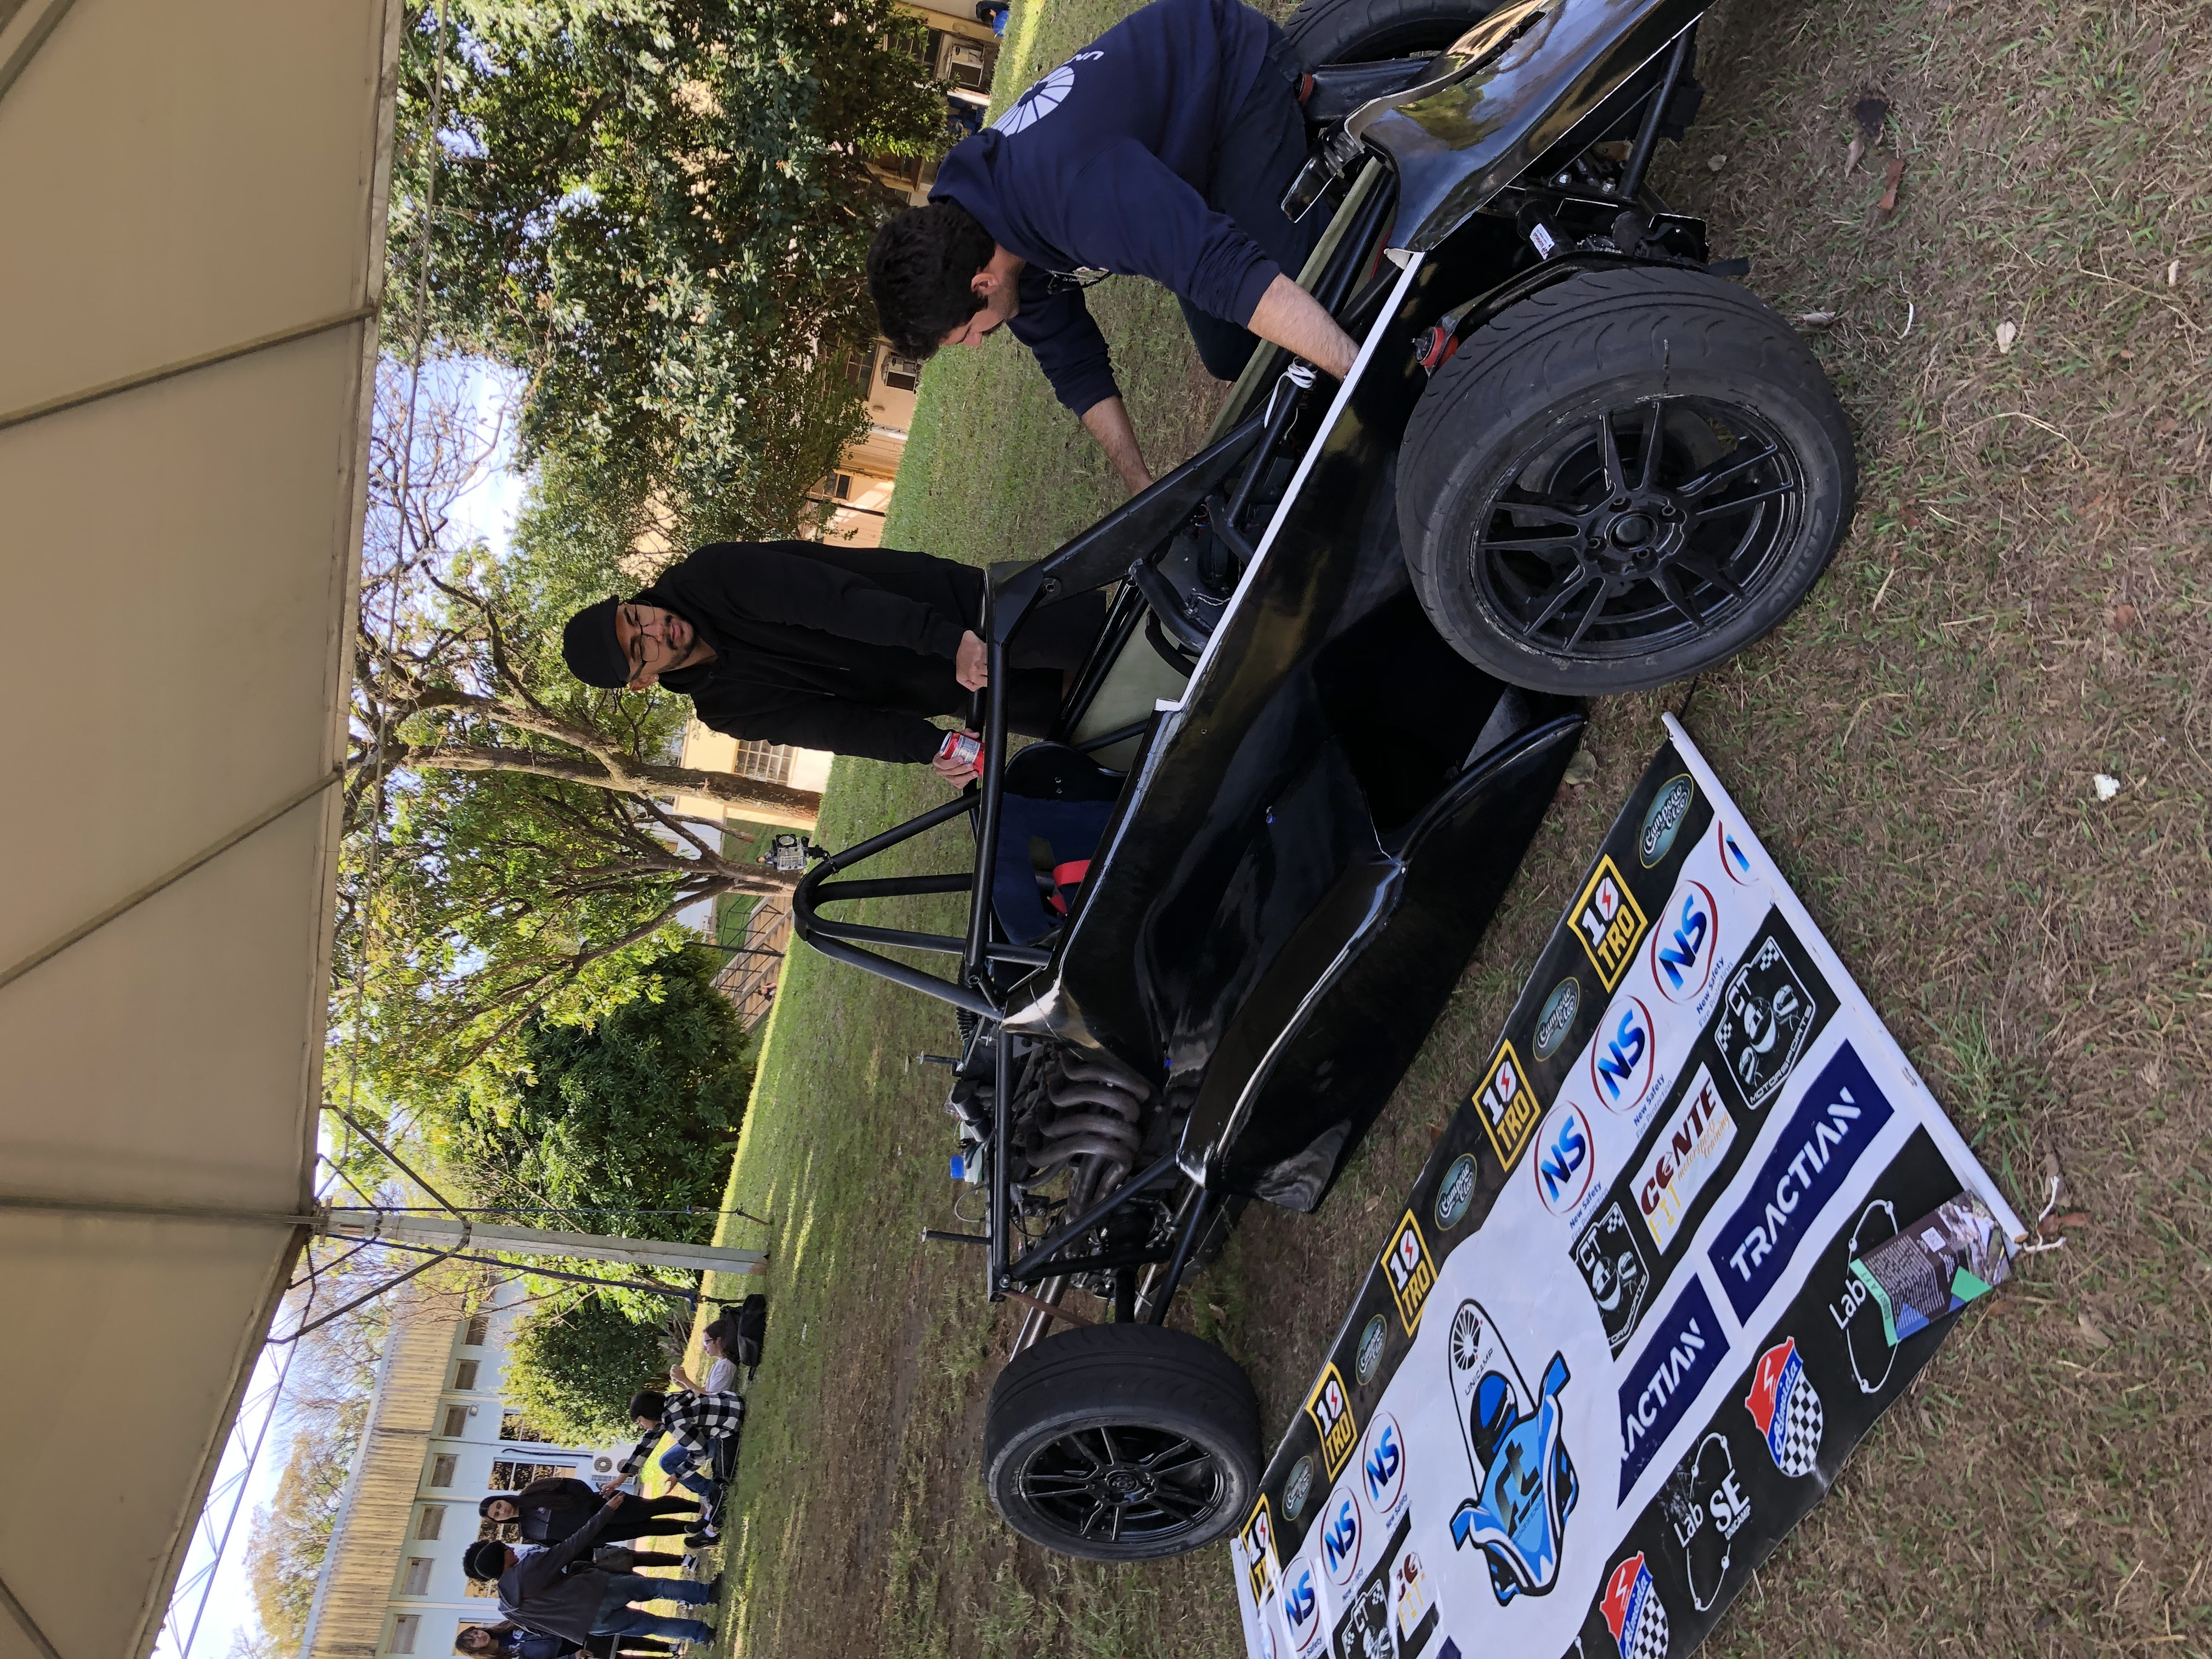
\includegraphics[width=0.7\linewidth,height=\textheight,keepaspectratio]{planejamento/exposicao-carro.jpg}

\begin{itemize}
\tightlist
\item
  \emph{Limeteria}: A equipe da Limeteria levou música para os dias do
  evento e alegrou os visitantes.
\end{itemize}

\includegraphics[width=0.7\linewidth,height=\textheight,keepaspectratio]{planejamento/limeteria.jpg}

\section{Alimentação e
segurança}\label{alimentauxe7uxe3o-e-seguranuxe7a}

Alguns \emph{foods trucks} estiveram presentes nos dias do evento para
fornecer opções de alimentação para os visitantes. Esses \emph{dood
trucks} foram organizados pela prefeitura do campus, junto ao Programa
\href{https://prefeituralimeira.unicamp.br/chefs-no-campus/}{chefs no
campus}. Dada a expectiva inicial da visita de várias escolas, foi
necessária a contratação temporária de mais dois vigias junto a empresa
terceirizada que presta serviços para a Unicamp/Limeira.

\section{Divulgação}\label{divulgauxe7uxe3o}

A divulgação do evento foi realizada em diversos meios.

\subsection{Folder}\label{folder}

Um folder foi elaborado para ser entregue aos visitantes nos dias do
evento. O folder contém informações sobre a FT e sobre os cursos de
graduação.

\includegraphics[width=0.9\linewidth,height=\textheight,keepaspectratio]{planejamento/folder-1.jpg}
\includegraphics[width=0.9\linewidth,height=\textheight,keepaspectratio]{planejamento/folder-2.jpg}

\subsection{Site}\label{site}

As principais informações sobre o evento foram disponibilizadas no
\href{https://wordpress.ft.unicamp.br/ftpa/}{site} do evento: cursos,
formas de inscrição dos visitantes, FAQ e a descrição das atividades do
evento.

\subsection{Escolas}\label{escolas}

Um convite foi enviado por email para aproximadamente 500 escolas de
diversas cidades. Informações sobre o evento e uma carta-convite do
diretor da FT foram apresentadas no email.

\begin{figure}[H]

{\centering \includegraphics[width=1\linewidth,height=\textheight,keepaspectratio]{planejamento/escolas-convite-500.png}

}

\caption{Distribuição das escolas convidadas por cidade.}

\end{figure}%

\begin{figure}[H]

{\centering \includegraphics[width=1\linewidth,height=\textheight,keepaspectratio]{planejamento/mapa-escolas.jpg}

}

\caption{Localização das escolas convidadas. O tamanho do círculo é
proporcional ao número de escolas convidadas na cidade.}

\end{figure}%

A mensagem enviada para as escolas é apresentada a seguir.

\begin{verbatim}
Prezado(a) Diretor(a) Fulano.

A Faculdade de Tecnologia da UNICAMP realizará o evento FT de Portas Abertas nos dias 13 e 14 de Junho em Limeira-SP.

Gostaríamos de convidar os alunos e professores do(a) nome da escola para nos visitar nesses dias.

Em anexo, apresentamos a carta-convite de nosso diretor com mais detalhes do evento.

Estamos também enviando o panfleto para divulgação do evento para a comunidade de sua escola, pais, alunos e familiares.

Para mais informações, acesse https://wordpress.ft.unicamp.br/ftpa/ .

É necessário realizar um agendamento da escola pelo link apresentado no site.

Será um prazer receber vocês aqui na FT/Unicamp! 

Comissão organizadora.
\end{verbatim}

\subsection{Jornais}\label{jornais}

O FT de Portas Abertas foi divulgado também no Jornal da Unicamp na
seção
\href{https://jornal.unicamp.br/agenda/2025/05/06/faculdade-de-tecnologia-realiza-a-edicao-2025-do-evento-ft-de-portas-abertas/\#:~:text=Nos\%20dias\%2013\%20e\%2014\%20de\%20junho\%20de\%202025\%2C\%20a,e\%20tecnol\%C3\%B3gica\%20oferecidas\%20pela\%20institui\%C3\%A7\%C3\%A3o.}{Agenda
Unicamp}, na \href{https://instagram.com/p/DJZ7ulQBLoF/}{Gazeta de
Limeira} e também no site da
\href{https://www.inova.unicamp.br/2025/05/inova-unicamp-estara-no-ft-de-portas-abertas-em-limeira/}{Inova}.

\section{Sinalização}\label{sinalizauxe7uxe3o}

Diversos banners foram confeccionados e distribuídos na FT para
facilitar a localização das atrações.

\begin{figure}[H]

{\centering 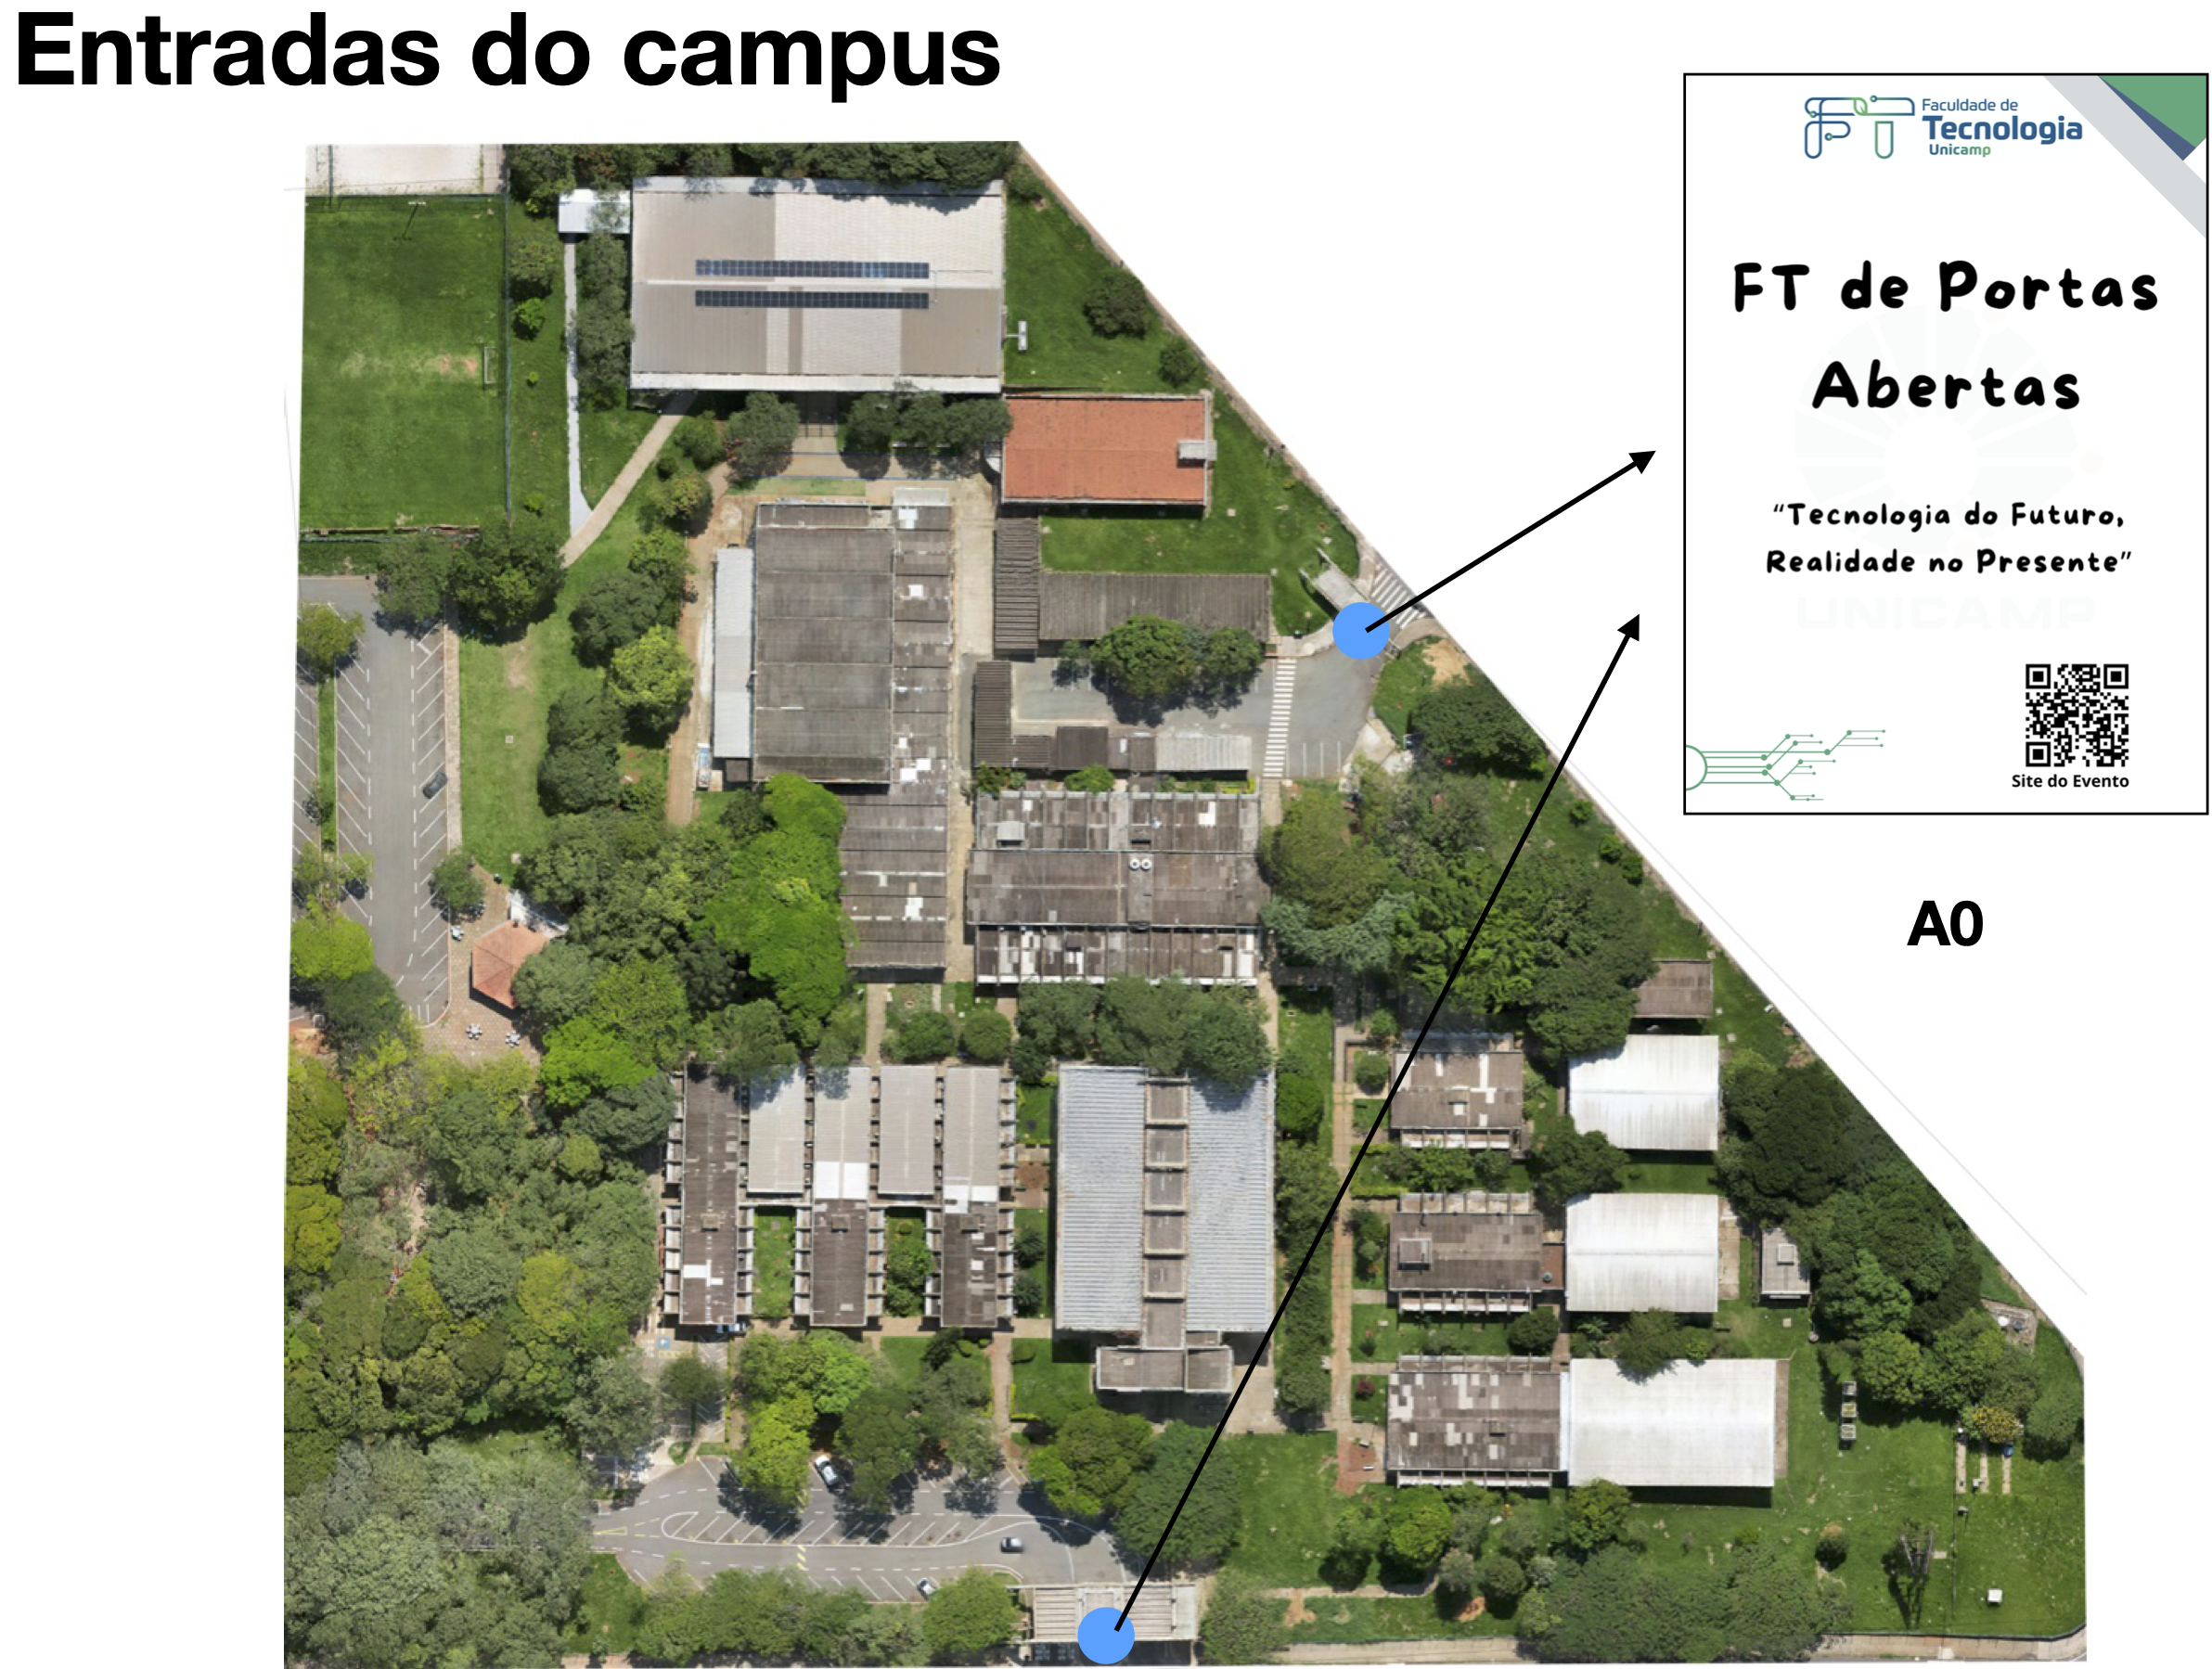
\includegraphics[width=0.8\linewidth,height=\textheight,keepaspectratio]{planejamento/banners-1.png}

}

\caption{Localização de banners (tamanho A0) de divulgação do evento nas
portarias do campus I.}

\end{figure}%

\begin{figure}[H]

{\centering 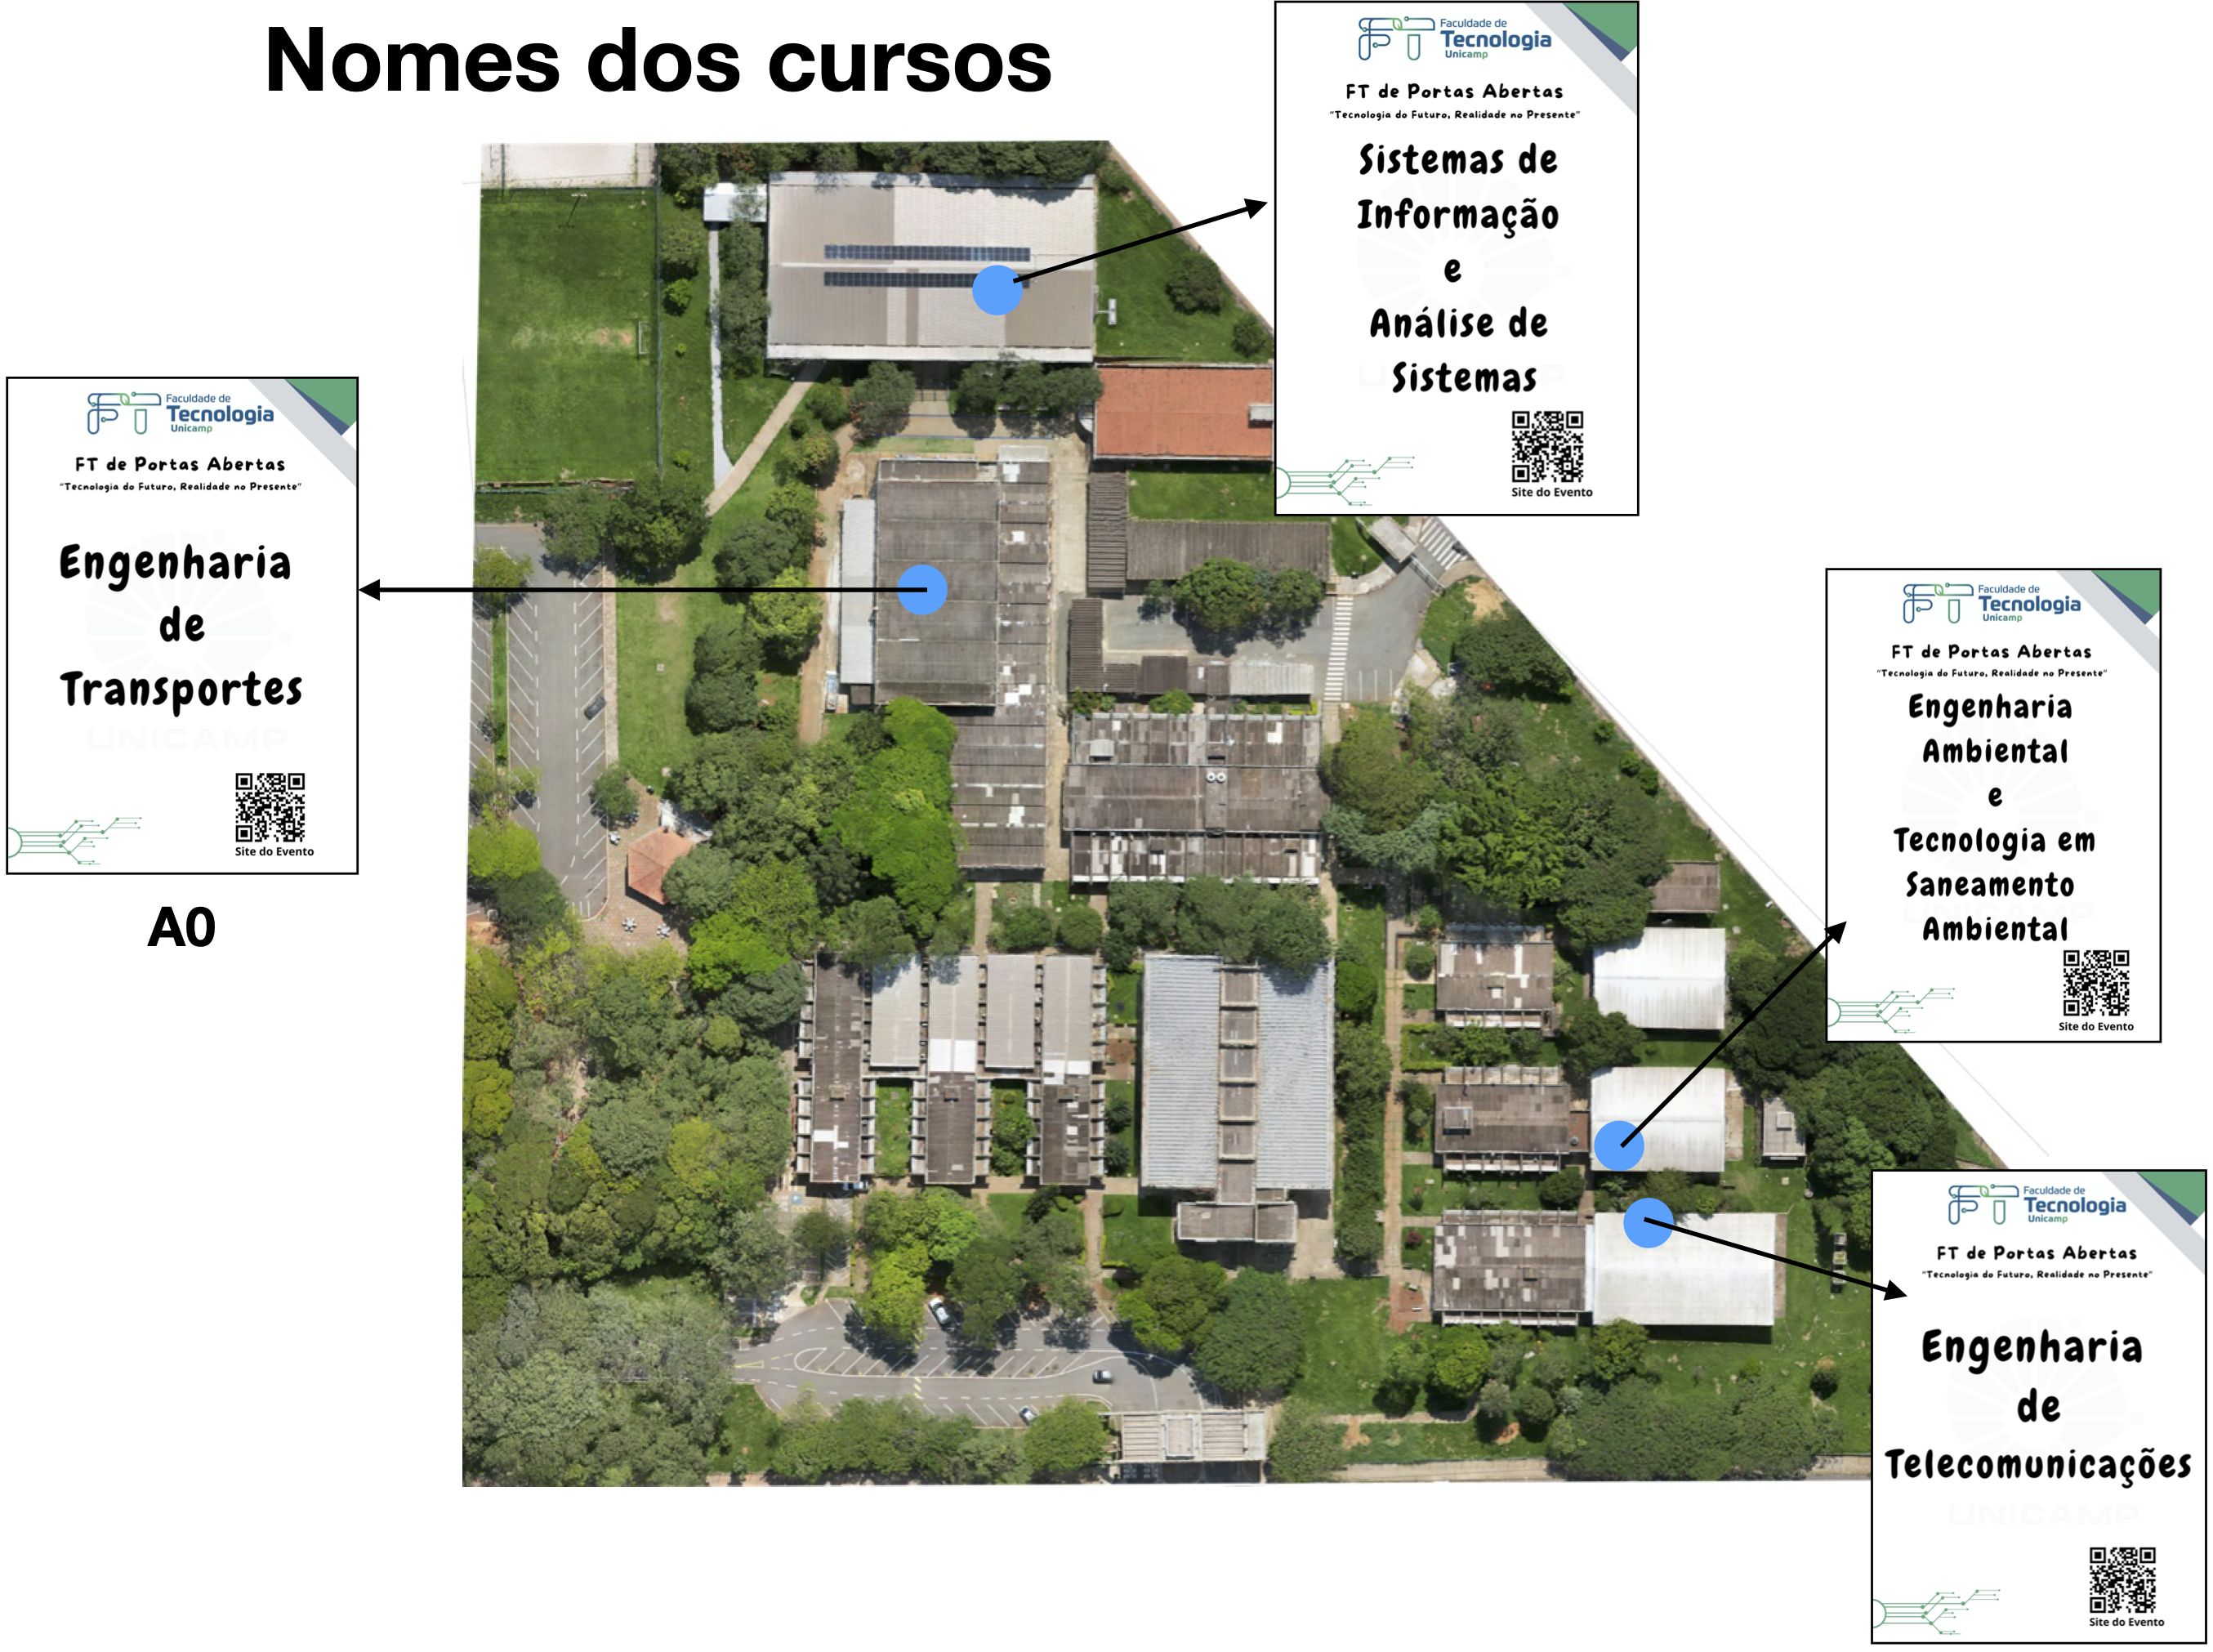
\includegraphics[width=0.8\linewidth,height=\textheight,keepaspectratio]{planejamento/banners-2.png}

}

\caption{Localização de banners (tamanho A0) de divulgação dos cursos
nas dependências da FT.}

\end{figure}%

\begin{figure}[H]

{\centering 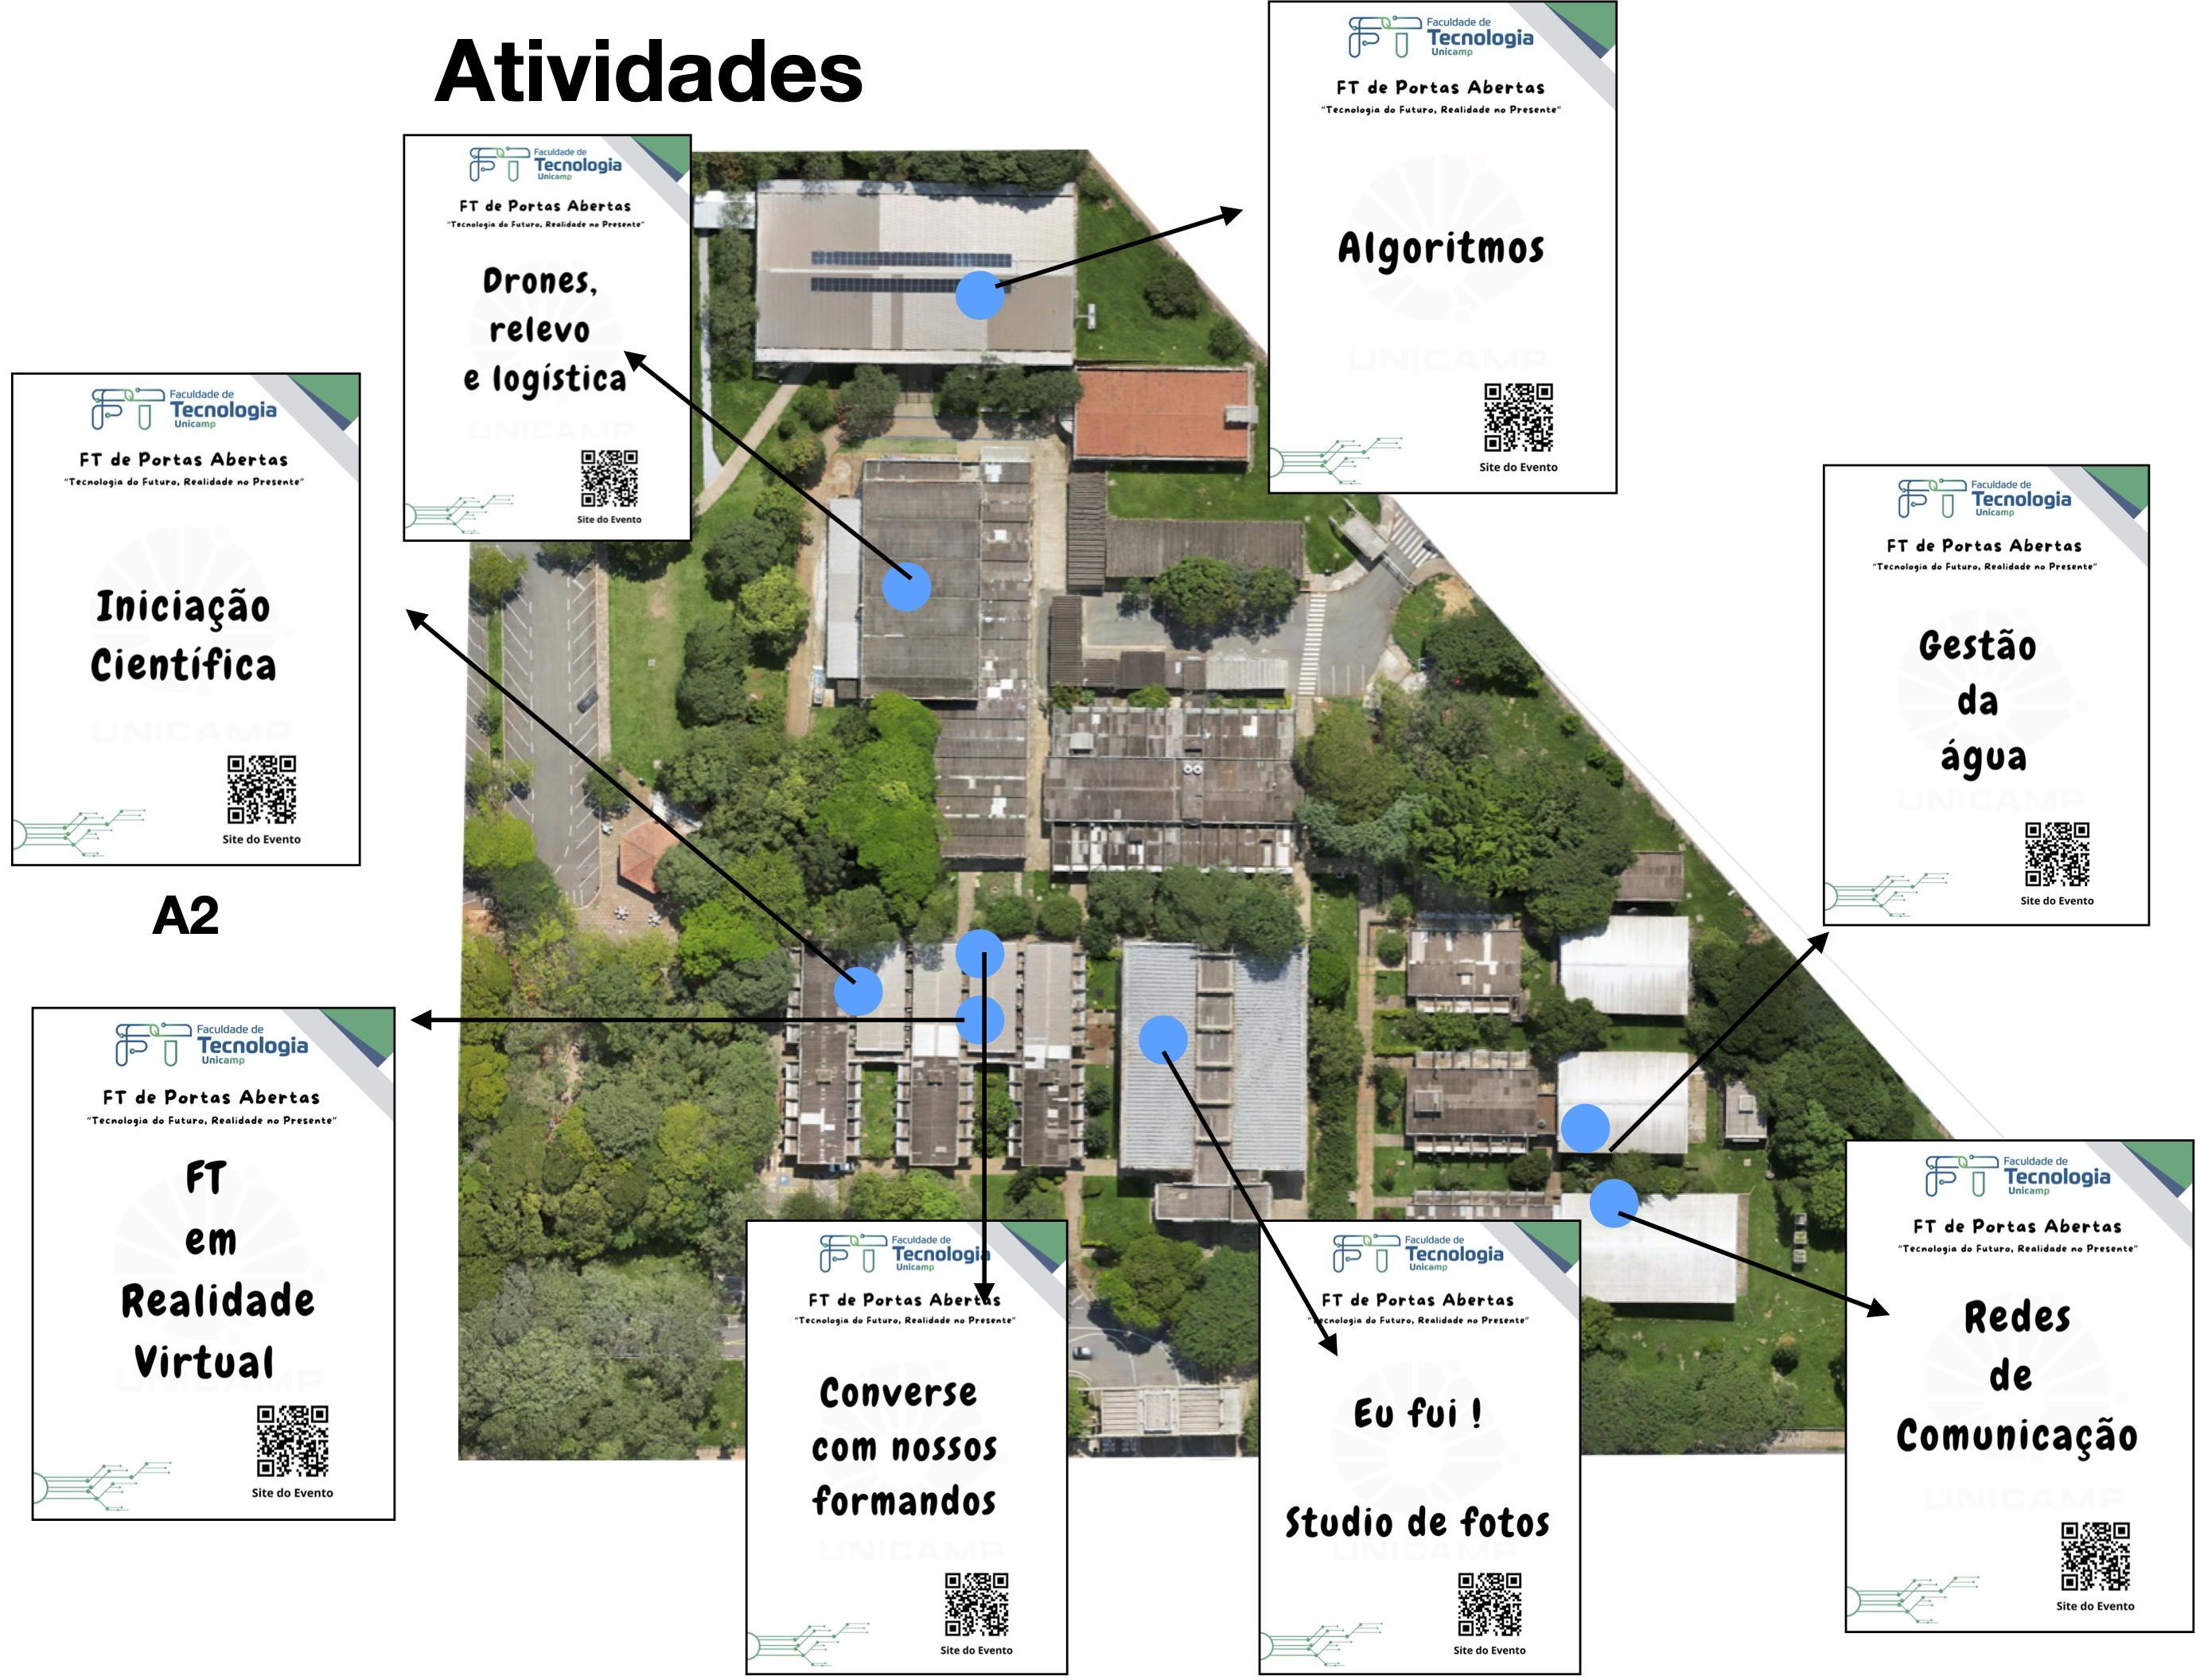
\includegraphics[width=0.8\linewidth,height=\textheight,keepaspectratio]{planejamento/banners-3.png}

}

\caption{Localização de banners (tamanho A2) de divulgação das atrações
nas dependências da FT.}

\end{figure}%

\section{Mídias digitais}\label{muxeddias-digitais}

Um \href{https://www.instagram.com/ftportasabertas/}{Instagram} para o
evento foi produzido pelos alunos, contendo informações sobre as
atrações e sobre os cursos da FT. Conteúdos também foram adicionados em
outras contas de Instagram da FT como, por exemplo, o
\href{https://www.instagram.com/reel/DKZt6T_xspD/}{convite para o
evento}. O formato desse convite foi depois
\href{https://www.instagram.com/p/DKk4qxtSHpM/?hl=pt}{reproduzido para
um evento de Extensão do IFGW/Unicamp}.

\section{Aplicativo}\label{aplicativo}

O FT de Portas Abertas também contou com um aplicativo para celular que
mostrava o mapa do campus, com indicações para as atrações, com
informações sobre os cursos e com a localização em tempo real do
visitante. O aplicativo pode ser usado via
\href{https://diversos-af313.web.app/ftpa/}{Web} ou em celulares Android
(\href{http://wordpress.ft.unicamp.br/ftpa/wp-content/uploads/sites/92/2025/06/ftpa_map.apk}{download
aqui}). O aplicativo foi desenvolvido pelo Prof.~Ulisses Martins Dias,
com dados obtidos por um drone fornecidos pelo Prof.~Vitor Molina.

\begin{figure}[H]

{\centering \includegraphics[width=1.1\linewidth,height=\textheight,keepaspectratio]{planejamento/app-mapa-Ulisses.jpg}

}

\caption{Tela do aplicativo do FT de Portas Abertas. Uma foto aérea da
FT é sobreposta ao mapa da FT. Locais das atrações são indicados em
roxo. O ícone no canto superior direito direciona o usuário para as
informações dos cursos da FT.}

\end{figure}%

\bookmarksetup{startatroot}

\chapter{Custos}\label{custos}

A comissão organizadora elaborou um documento para a Pró-reitoria de
Graduação, solicitando R\$ 45.794,32 para a realização do evento. Esses
recursos seriam originalmente para adquirir camisetas para equipe
organizadora e de suporte, contratar serviços gráficos, pagar diárias
para monitores, pagar aluguel de tenda, imprimir adesivos para placas de
identificação visual no campus, adquirir módulo didático de mini estação
de tratamento de água, material de consumo para impressora 3D e licença
de jogos para uma atividade do curso de Engenharia de Transportes. Os
recursos foram aprovados integralmente.

Os itens efetivamente adquiridos/contratados estão listados na tabela a
seguir, num custo total final de \textbf{R\$ 33.370,25}, 73\% do valor
inicialmente aprovado.

\begin{longtable}[]{@{}ll@{}}
\caption{Custos do FTPA 2025.}\tabularnewline
\toprule\noalign{}
Item & Valor (R\$) \\
\midrule\noalign{}
\endfirsthead
\toprule\noalign{}
Item & Valor (R\$) \\
\midrule\noalign{}
\endhead
\bottomrule\noalign{}
\endlastfoot
50 Camisetas & 2.400,00 \\
Tenda & 6.900,00 \\
34 diárias para monitores & 4.020,24 \\
Mini estação de tratamento & 10.590,00 \\
1000 Folders & 1.220,00 \\
14 Banners & 463,02 \\
Insumos para impressora 3D & 463,00 \\
Transporte para retirada dos insumos & 371,21 \\
2 Cabos RV & 369,00 \\
Itens de almoxarifado & 5,46 \\
Coffee-break & 1.656,00 \\
Segurança & 4.917,78 \\
TOTAL & 33.370,25 \\
\end{longtable}

A confecção das camisetas, banners, folders, a contratação da tenda e a
aquisição da mini estação de tratamento de água tiveram valores menores
do que os estimados inicialmente. Devido ao tempo de manufatura, a
estação não chegou a tempo do evento, porém poderá ser utilizada em
edições futuras, no próprio UPA e também em aulas de graduação. Os
adesivos para placas e a licenças de jogos não foram adquiridos. Por
outro lado, a contração de segurança adicional para o evento, que não
estava incluída no planejamento financeiro inicial, teve que ser feita,
dada a estimativa de público para o evento. O coffee-break para os
monitores também foi um item adicionado para fornecer-lhes uma
alimentação nos dias do evento, sem obrigá-los a ter que sair do campus
para isso.

\bookmarksetup{startatroot}

\chapter{Visitantes}\label{visitantes}

\section{Escolas}\label{escolas-1}

Escolas de nove cidades participaram do FT de Portas Abertas 2025,
trazendo em torno de 400 alunos:

\begin{enumerate}
\def\labelenumi{\arabic{enumi}.}
\item
  Colégio Jandyra Antunes Rosa, Limeira (15 alunos)
\item
  Cotil, Limeira (40)
\item
  Anglo Alante Araras, Araras (40)
\item
  Escola SESI Indaiatuba, Indaiatuba (80)
\item
  Objetivo Itupeva, Itupeva (42)
\item
  ETEC, Monte Mor (46)
\item
  Colégio Ideal, Santa Bárbara d'Oeste (17)
\item
  Instituto São José, São José dos Campos (45)
\item
  Colégio Dom Aguirre, Sorocaba (48)
\item
  COC, Leme (31)
\end{enumerate}

\section{Público em geral}\label{puxfablico-em-geral}

Famílias também participaram do FT de Portas Abertas.

\begin{figure}[H]

{\centering \includegraphics[width=0.7\linewidth,height=\textheight,keepaspectratio]{visitantes/foto-familia.jpg}

}

\caption{Família em atividade com realidade virtual.}

\end{figure}%

\begin{figure}[H]

{\centering 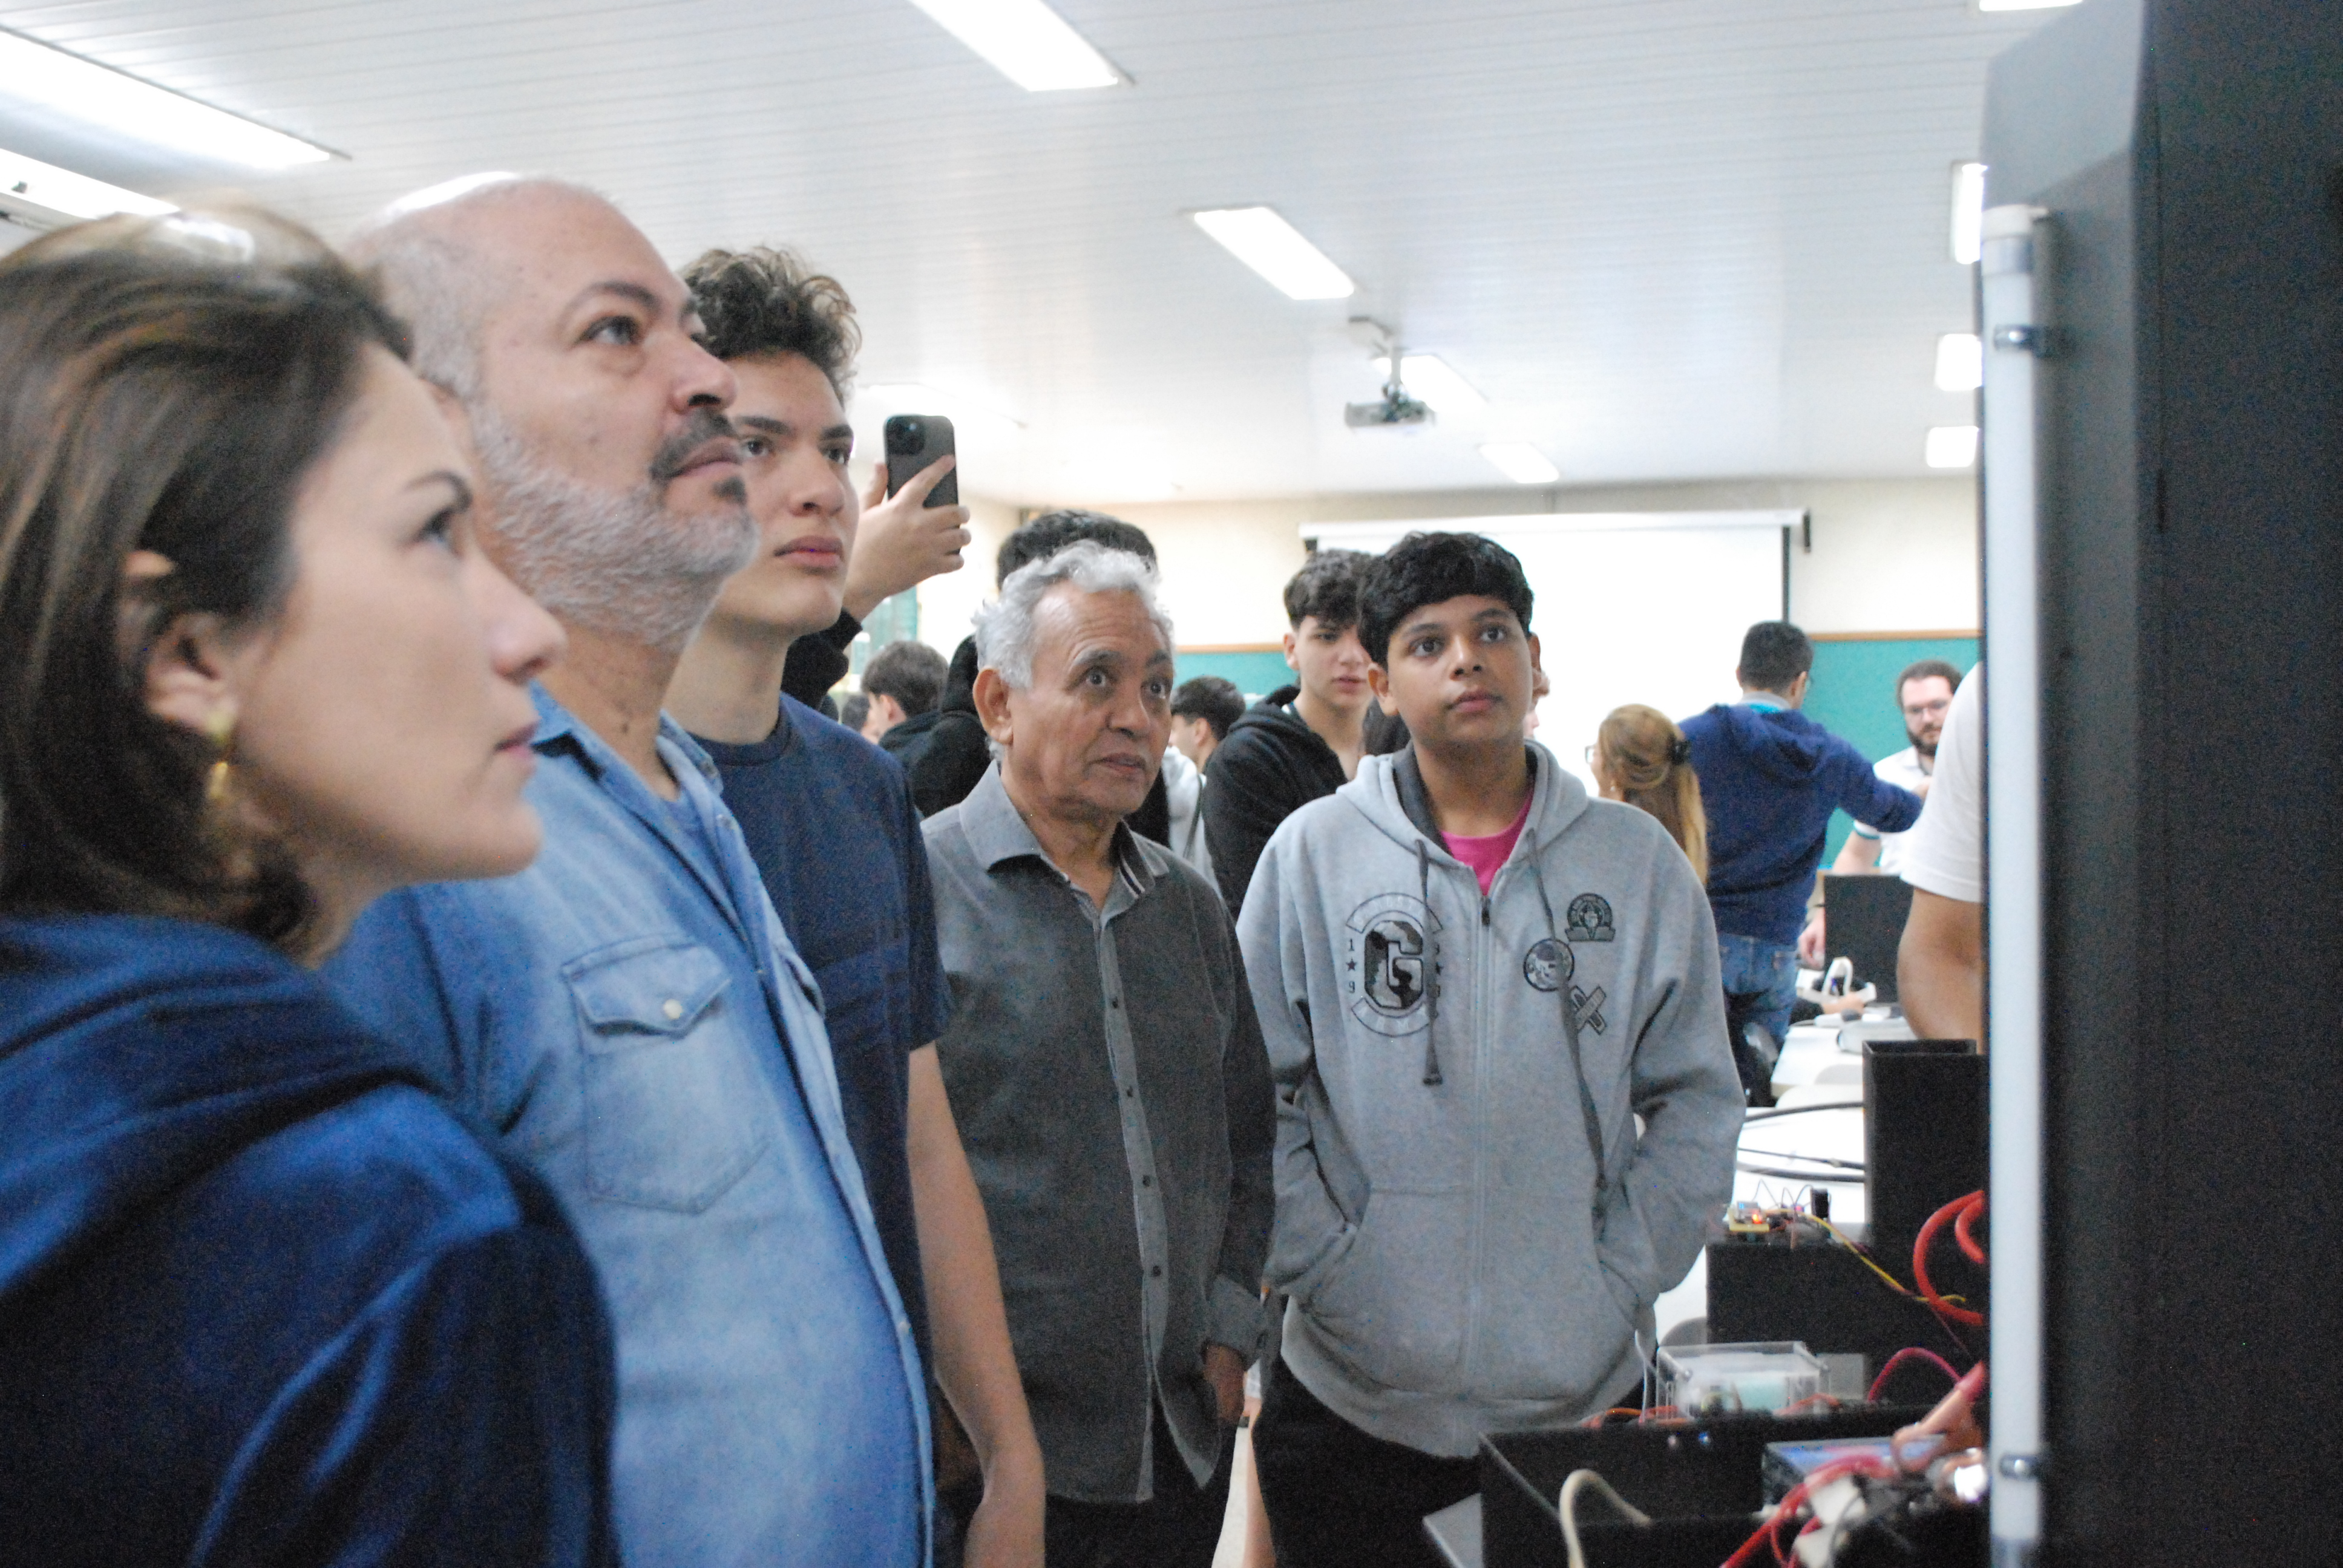
\includegraphics[width=0.7\linewidth,height=\textheight,keepaspectratio]{visitantes/foto-familia-2.jpg}

}

\caption{Família em atividade de robótica.}

\end{figure}%

\url{depoimento-1.mp4}

Depoimento de família de Jundiaí.

\bookmarksetup{startatroot}

\chapter{Recomendações}\label{recomendauxe7uxf5es}

A realização da FT de Portas Abertas (FTPA) representa uma das
principais iniciativas da Faculdade de Tecnologia da Unicamp voltadas à
divulgação dos cursos de graduação e à aproximação com estudantes do
Ensino Médio, professores e a comunidade em geral. Mais do que um evento
de recepção e apresentação institucional, a FTPA busca cumprir um papel
estratégico: ampliar a visibilidade da FT, fortalecer sua inserção
social e contribuir para a atração de novos alunos para seus cursos.

Durante a execução do FTPA, diversos pontos foram percebidos que
poderiam ser melhorados para edições futuras. A seguir, listamos esses
pontos.

\section{Comissão Permanente}\label{comissuxe3o-permanente}

A comissão organizadora foi instituída em 16/12/2024 e a primeira
reunião ocorreu no dia 6/01/2025. Dada a importância do evento para a
própria FT, vimos a necessidade de mais tempo para a organização. Parte
disso se deve ao fato de ser o primeiro evento desse tipo na FT, o que
requereu aprender muitos processos, tomando muito tempo da comissão. Uma
sugestão seria instituir uma comissão permanente que poderia trabalhar
ao longo do ano para o planejamento e divulgação do evento.

\section{Composição da comissão
organizadora}\label{composiuxe7uxe3o-da-comissuxe3o-organizadora}

A participação dos alunos foi essencial para o sucesso do FT de Portas
Abertas. A inclusão de alunos na comissão organizadora iria facilitar a
comunicação e planejamento das atividades com a equipe de suporte
(monitores).

\section{Divisão de tarefas na
comissão}\label{divisuxe3o-de-tarefas-na-comissuxe3o}

As tarefas ficaram muito concentradas para o presidente da comissão. A
sugestão para o próximo presidente, para o próprio bem dele, seria
dividir a equipe em grupos para atividades específicas como, por
exemplo, (a) compras/contratação, (b) divulgação nas escolas, (c) página
e mídias sociais, (d) logística e (e) atrações.

\section{Convênio com prefeitura de
Limeira}\label{convuxeanio-com-prefeitura-de-limeira}

A ausência de escolas públicas de Limeira no evento trouxe um alerta.
Apesar de esforços na divulgação via email e presencial em algumas
escolas, uma maior participação poderá ser alcançada estabelecendo-se um
convênio com a Prefeitura de Limeira. Isso deve ser feito com
antecedência, já que trâmites nesse sentido podem demorar. Uma outra
ação complementar seria contratar ônibus para trazer os estudantes de
algumas escolas de Limeira para o evento. Recursos da curricularização
da extensão poderiam ser usados para este fim.

\section{Parceria com o Cotil}\label{parceria-com-o-cotil}

Apesar da divulgação do evento para a diretoria acadêmica do Cotil, a
participação ocorreu apenas com uma turma de alunos, trazida por
iniciativa individual de um professor. Realizar a divulgação do FT de
Portas abertas junto ao Cotil deve ser uma prioridade para a próxima
comissão organizadora.

\section{Horário das atrações}\label{horuxe1rio-das-atrauxe7uxf5es}

As dinâmicas de cada curso e as outras atividades do evento
proporcionaram boas atrações para os visitantes. Definir horários para
essas atrações e divulgá-los no site do evento irá facilitar a
organização da logística do evento. Estabelecer os horários de início
das trilhas ajudará as escolas a organizarem suas vindas para
aproveitarem melhor o evento. Uma trilha de aproximadamente 2h por
período permitirá uma melhor circulação pelo campus. Além disso, iniciar
a trilha às 10h e 14h permite que um número suficiente de visitantes
esteja presente para a trilha. Além da trilha das dinâmicas, será
importante definir atividades para a visitação livre, caso o visitante
não chegue a tempo do início da trilha. A visitação livre deve ser
possível em qualquer período e é importante principalmente para famílias
ou grupos menores que chegam aleatoriamente ao longo do dia. Nessa
definição de atrações, será importante também estabelecer e informar o
horário de almoço para a equipe de monitores.

\section{Logística}\label{loguxedstica}

O processo de levar os grupos para as dinâmicas foi o mais estressante,
uma vez que lidávamos com a incerteza da quantidade de alunos e o
momento que chegariam para o evento. Estabelecer horários fixos para o
início das trilhas pode ajudar. Ter parte da equipe de logística para
atender grupos atrasados para as trilhas pode melhorar a circulação.
Adaptar o aplicativo do evento para auxiliar na logística poderá
fornecer uma ferramenta de organização.

\section{Aumento das atrações}\label{aumento-das-atrauxe7uxf5es}

A visita nos laborórios de pesquisa e de extensão pode ser mais
explorada. Isso proporcionará mais opções para o visitante ao mesmo
tempo que ajuda divulgar ainda mais as atividades desenvolvidas na FT. A
apresentação dos laboratórios pode ser feita com a ajuda de
pós-graduandos e de bolsistas de iniciação científica.

\section{Documentação financeira}\label{documentauxe7uxe3o-financeira}

O pagamento de diárias para os monitores exigiu um aprendizado do setor
financeiro da FT, dado o número grande de pedidos simultâneos. Para o
processo de pagamento, eram necessários os seguintes documentos (em
formato PDF): (a) planilha com as informações (Nome completo; CPF;
Número de matrícula; Dados bancários; Valores); (b) prospecto do evento;
(c) atestado de matrícula emitido pela DAC, referente ao período letivo
em curso; (d) comprovante de endereço (pode ser utilizada a declaração
firmada pelo próprio interessado, nos termos da Lei Federal nº
7.115/83); (e) informação do interessado indicando o banco, agência e
conta corrente em que será creditado o pagamento.

Percebemos que o processo de envio de documentos foi facilitado
criando-se um Google Forms para obter as informações para os documentos
(a), (c) e (d). Como comprovante de endereço, vimos que é mais fácil
solicitar aos alunos o envio da seguinte declaração, assinada
digitalmente:

\begin{center}\rule{0.5\linewidth}{0.5pt}\end{center}

DECLARAÇÃO DE RESIDÊNCIA

Eu,\_\_\_\_\_\_\_\_\_\_\_\_\_\_\_\_\_\_\_\_\_\_\_\_\_\_\_\_\_\_\_\_\_\_\_\_\_\_\_\_\_\_\_\_\_\_\_\_\_\_\_\_\_\_\_\_\_\_
\_\_\_\_\_\_\_\_\_\_\_\_\_\_\_\_\_, CPF nº
\_\_\_\_\_\_\_\_\_\_\_\_\_\_\_\_\_\_\_\_\_\_\_\_\_ RG nº
\_\_\_\_\_\_\_\_\_\_\_\_\_\_\_\_\_\_ Órgão Exped.
\_\_\_\_\_\_\_\_\_\_\_\_, telefone
(\_\_\_\_\_)\_\_\_\_\_\_\_\_\_\_\_\_\_\_\_\_\_\_\_, na falta de
documentos para comprovação de residência, em conformidade com o
disposto na Lei 7.115, de 29 de agosto de 1983, DECLARO para os devidos
fins, sob penas da Lei, ser residente e domiciliado no endereço
\_\_\_\_\_\_\_\_\_\_\_\_\_\_\_\_\_\_\_\_\_\_\_\_\_\_\_\_\_\_\_\_\_\_\_\_\_\_\_\_\_\_\_\_
\_\_\_\_\_\_\_\_\_\_\_\_\_\_\_\_\_\_\_\_\_\_\_\_\_\_\_\_\_\_\_\_\_\_\_\_\_\_\_\_\_\_\_\_\_\_\_\_\_\_\_\_\_\_\_\_\_\_\_\_\_\_\_\_\_\_\_\_\_\_\_\_\_.
Por ser verdade, firmo a presente declaração para que produza os efeitos
legais, ciente de que a falsidade de seu conteúdo pode implicar na
imputação de sanções civis, administrativas, bem como na sanção penal
prevista no art. 299 do Código Penal, conforme transcrição abaixo:

``Art. 299 -- Omitir, em documento público ou particular, declaração que
nele deveria constar, ou nele inserir ou fazer inserir declaração falsa
ou diversa da que devia ser escrita, com o fim de prejudicar direito,
criar obrigação ou alterar a verdade sobre o fato juridicamente
relevante. Pena: reclusão de 1 (um) a 5 (cinco) anos e multa, se o
documento é público e reclusão de 1 (um) a 3 (três) anos, se o documento
é particular''

\_\_\_\_\_\_\_\_\_\_\_\_\_\_\_\_\_\_\_\_\_\_\_\_\_\_\_\_\_,
\_\_\_\_\_\_\_\_\_/\_\_\_\_\_\_\_\_\_/\_\_\_\_\_\_\_\_\_\_.

Local Data

\_\_\_\_\_\_\_\_\_\_\_\_\_\_\_\_\_\_\_\_\_.

Assinatura do Declarante
\_\_\_\_\_\_\_\_\_\_\_\_\_\_\_\_\_\_\_\_\_\_\_\_\_\_\_\_\_\_\_\_\_\_\_\_\_\_\_\_\_

O endereço informado deve ser o mesmo cadastrado na DAC.

Para a informação bancária do aluno, a forma mais eficiente foi por meio
do envio, pelo aluno, para o setor financeiro de um email com o seguinte
conteúdo:

\begin{center}\rule{0.5\linewidth}{0.5pt}\end{center}

Esses são os dados da minha conta:

Banco:\_\_\_\_\_\_\_\_\_\_\_\_\_\_\_\_\_\_.

Agência: \_\_\_\_\_\_\_\_\_\_\_\_\_\_\_\_\_.

Conta: \_\_\_\_\_\_\_\_\_\_\_\_\_\_\_\_\_.

Nome do aluno

\begin{center}\rule{0.5\linewidth}{0.5pt}\end{center}

Finalmente, os documentos (c), (d) e (e) devem ser agrupados num único
arquivo PDF para facilitar a inserção no sistema de pagamento da
Unicamp.

\section{Melhorias no campus}\label{melhorias-no-campus}

A constante melhoria do campus, seja ela para a visitação da comunidade
externa, seja ela para o uso da comunidade de interna, deve ser sempre
buscado pela Diretoria da FT e pela prefeitura do campus. Durante a
organização do FT de Portas Abertas, apontamos vários locais do campus
que poderiam ser melhorados. Exemplos de três deles são mostrados a
seguir.

\begin{figure}[H]

{\centering \includegraphics[width=0.6\linewidth,height=\textheight,keepaspectratio]{recomendacoes/melhoria-1.png}

}

\caption{Limpeza das paredes externas e remoção de lixo. As setas em cor
vermelho destacam a necessidade da limpeza e pintura das paredes.}

\end{figure}%

\begin{figure}[H]

{\centering \includegraphics[width=0.6\linewidth,height=\textheight,keepaspectratio]{recomendacoes/melhoria-2.png}

}

\caption{Remoção de itens inutilizados.}

\end{figure}%

\begin{figure}[H]

{\centering \includegraphics[width=0.6\linewidth,height=\textheight,keepaspectratio]{recomendacoes/melhoria-3.png}

}

\caption{Limpeza de parede e revitalização de placas informativas do
campus.}

\end{figure}%

Em relação às placas informativas, a comissão elaborou novos designs
para elas e apresentou-os para a prefeitura do campus. No entanto,
nenhum retorno sobre isso foi obtido e as modificações não foram
realizadas.

\begin{figure}[H]

{\centering \includegraphics[width=0.6\linewidth,height=\textheight,keepaspectratio]{recomendacoes/placas.png}

}

\caption{Sugestão da comissão para as novas placas informativas do
campus.}

\end{figure}%

\section{Ampliação da participação da comunidade
interna}\label{ampliauxe7uxe3o-da-participauxe7uxe3o-da-comunidade-interna}

A FT de Portas Abertas beneficia a própria FT. Ações para aumentar a
adesão da comunidade interna devem ser implantadas para expandir o
número de atrações no evento e aproximar a FT da comunidade externa. Por
exemplo, a participação de laboratórios de pesquisa foi pequena no
evento. Visitas nos laboratórios ou mesmo pequenos estandes, para expor
parte da pesquisa feita, poderiam despertar interesse dos visitantes.

\section{Acompanhamento e avaliação do impacto do
evento}\label{acompanhamento-e-avaliauxe7uxe3o-do-impacto-do-evento}

Estabelecer mecanismos sistemáticos de acompanhamento e avaliação do
impacto do FTPA é fundamental para que ela atinja seus objetivos. A
partir da coleta e análise de dados, como a percepção dos visitantes, a
influência do evento na escolha dos cursos e a evolução do número de
inscritos e ingressantes, será possível mensurar a eficácia da FTPA
enquanto ação de divulgação institucional e de fortalecimento da
graduação.

Além de subsidiar a melhoria contínua do evento, o monitoramento
sistemático permitirá à FT:

\begin{itemize}
\item
  Ajustar suas estratégias de comunicação e interação com escolas e
  comunidades;
\item
  Avaliar a efetividade do investimento institucional e dos apoios
  recebidos;
\item
  Identificar tendências e potencializar a atração de novos estudantes;
\end{itemize}

Espera-se que, ao longo dos anos, a FTPA consolide-se como uma ação
culturalmente reconhecida pela comunidade, estabelecendo um vínculo
entre a FT e os estudantes do Ensino Médio. A construção desse caráter
institucional visa não apenas a aproximação social, mas também o
fortalecimento da imagem da FT como referência em formação tecnológica e
de engenharia.

Nesse sentido, uma das primeiras e mais objetivas formas de
acompanhamento da efetividade do evento consiste na análise sistemática
dos dados oficiais da COMVEST, acompanhando a evolução das inscrições
nos processos seletivos da Unicamp, bem como a relação candidato/vaga
dos cursos da FT. O monitoramento desses indicadores ao longo dos anos
permitirá verificar eventuais correlações entre a realização da FTPA e o
interesse dos estudantes pelos cursos de graduação da unidade.

Além desse acompanhamento, são ainda sugeridas duas outras formas de
avaliação do evento:

\begin{enumerate}
\def\labelenumi{\arabic{enumi}.}
\item
  Avaliação imediata à realização do evento por meio de questionário a
  ser preenchido pelas escolas participantes: O questionário dará
  informações importantes sobre a eficiência do evento, bem como será
  capaz de listar melhorias para as próximas edições. Uma sugestão de
  questionário pode ser visto \href{questionario-1.txt}{aqui}.
\item
  Avaliação Longitudinal --- Monitoramento de Ingressantes: Identificar,
  junto aos alunos calouros se a FT de Portas Abertas foi um fator
  relevante na decisão dos ingressantes. Para isso, podem ser usados,
  por exemplo, questionários já existentes da FT e que já são aplicados
  para calouros no dia da matrícula. Uma sugestão de questionário pode
  ser visto \href{./questionario-2.txt}{aqui}.
\end{enumerate}

\bookmarksetup{startatroot}

\chapter{Agradecimentos}\label{agradecimentos}

Gostaríamos de agradecer os professores e funcionários da FT que
contribuíram direta ou indiretamente para o FT de Portas Abertas. Um
agradecimento especial também aos alunos listados a seguir que, sem a
participação deles, o evento não teria sido possível.

\begin{enumerate}
\def\labelenumi{\arabic{enumi}.}
\tightlist
\item
  Adriano Baumgarte Bassani Filho
\item
  Amanda Feldman
\item
  Ana Carolina Cunha Caracini
\item
  Ana Clara Jesus de Andrade
\item
  Ana Júlia de Oliveira Gotto
\item
  Ana Júlia Pichirilo Mautner
\item
  Ana Julia Santos
\item
  Ana Julia Villas Boas
\item
  Andrey Moura Gouvêa
\item
  Andrey Santana Castilho
\item
  Anna Julia Marinho Barbosa
\item
  Arthur Luiz Lopes Araujo
\item
  Auriane Nayara da Silva
\item
  Bárbara Helóra Nigra Táparo
\item
  Beatriz Amaral
\item
  Beatriz Cristina de Oliveira Jatobá
\item
  Beatriz Santos de Melloi
\item
  Bianca Silva da Nobrega
\item
  Bruno Ribeiro Silva
\item
  Camila Almeida Champi
\item
  Carlos Daniel Nunes de Abreu
\item
  Caroline Sorg
\item
  Celio Benhami Junior
\item
  Cicero Eduardo Campos Leite Bispo
\item
  Daniel Matias de Sousa Nunes
\item
  Daniel Riquetto da Silva
\item
  Eduarda Ortiz Almeida
\item
  Erick Gabriel Afonso Mantoan
\item
  Ester Souza Gomes
\item
  Felipe de Souza Conde
\item
  Fernanda Souza Pedreira
\item
  Fernando Frias Salim
\item
  Gabriel Abdalla Navarro
\item
  Gabriel Cerqueira Pires
\item
  Gabriel Gaudio Saraiva
\item
  Gabriela Maura Rodrigues
\item
  Gabriela Nogueira
\item
  Giovanni da Silva Virginio Brandão
\item
  Henrique de Toledo Franca Bueno
\item
  Hibrael Zonta de Carvalho
\item
  Hugo Alexandre Strassa
\item
  Hugo de Paula Oliveira
\item
  Hugo Gomes de La Fuente
\item
  Isabella Alves de Almeida
\item
  Isadora Lacerda de Oliveira
\item
  Isadora Morcelli Loureiro
\item
  Ísis G. Vasconcelos
\item
  Jamily Macedo Moreira
\item
  Jhenyffer Cristina dos Santos
\item
  João Guilherme Fernandes Frota
\item
  João Vitor Tito da Paixão
\item
  José Henrique Lessa Vieira
\item
  Joyce Soares Martins
\item
  Juan Carlos Rezende Canha
\item
  Julia Coqueiro Ho
\item
  Julia Fernandes dos Santos
\item
  Kahlil Campos
\item
  ⁠Karol Heydy Yantas Espinoza
\item
  Laira Maria Carvalho Santos
\item
  Larissa Helena Franceli
\item
  Leonardo Basset Figueiredo Pereira
\item
  Leonardo Bonfá Schroeder
\item
  Leonardo Hideaki Sasaki Kopczynski
\item
  Lívia Fernandes Dalfré
\item
  Lorena Testa Avelar
\item
  Lucas de Jesus Mota Ferreira
\item
  Lucas de Oliveira Lopes Cardoso
\item
  Lucas Gabriel Hernandez Nogueira
\item
  Lucas Martins Paiva
\item
  Luiz Gustavo Esperidião de São José
\item
  Manuela Lima Leite da Cruz
\item
  Marcos Revejes Pedroso
\item
  Maria Clara Marsola Paulini
\item
  Maria Eduarda Cerqueira Santos
\item
  Maria Eduarda de Souza Gomes
\item
  Maria Eduarda Rodrigues dos Santos
\item
  ⁠Maria Fernanda Dias Alves
\item
  Maria Laura Alves de Souza Cruvinel
\item
  Maria Stella Dias Barbosa
\item
  Martim Rudge Machado
\item
  Matheus Lima de Oliveira
\item
  Matheus Placideli Reghini Scola
\item
  Matheus Rafael Dos Santos Nascimento
\item
  Mirella dos Santos Nascimento
\item
  Murilo Bertolini Montoni
\item
  Murilo de Carvalho Ximenes
\item
  Nasser Nasser Fares
\item
  Natalia Martins de Paiva
\item
  Nina de Oliveira Venell
\item
  Otavio Andrade Freiras Moraes
\item
  Pamela Anny Marques da Silva
\item
  Paulo Vitor Lopes Lima
\item
  Pedro dos Santos Conceição
\item
  Pedro Henrique Skemas Gomes de Britto
\item
  Pedro Henrique Souza dos~Santos
\item
  Pedro Luiz de Jesus da Silva Vieira
\item
  Phillipi Poloni
\item
  Rafael Henrique Pereira de Souza
\item
  Raissa Toassa Martinelli
\item
  Rebecca Vasques
\item
  Samir de Souza Francisco
\item
  Samuel Germiniani
\item
  Samuel Lucena Silva e Costa
\item
  Sergio Carlos de Sousa Gregorio Junior
\item
  Sofia Carnevalli Lopes
\item
  Sofia Helena Sato
\item
  Sofia Perboni Domingos
\item
  Tácio Mendes dos Santos Felix
\item
  Talita Lima
\item
  Thaís Araújo Alcântara
\item
  Thiago Camargo de Almeida
\item
  Victor Gavazzi
\item
  Vinicius Eiki Venâncio Tanizaki
\item
  Vinícius Iutaka Nogueira Fujioka
\item
  Vithoria Neves Garcia
\item
  Vitor Nogueira de Toledo
\item
  Yngrid Lohane Gouveia Lombelo
\item
  Yuri Santana Costa
\end{enumerate}

\begin{figure}[H]

{\centering \includegraphics[width=0.8\linewidth,height=\textheight,keepaspectratio]{agradecimentos/foto-equipe.jpg}

}

\caption{Parte da equipe do FT de Portas Abertas 2025.}

\end{figure}%

\bookmarksetup{startatroot}

\chapter{Considerações finais}\label{considerauxe7uxf5es-finais}

O FT de Portas Abertas cumpriu seu objetivo de apresentar as atividades
da FT para a comunidade externa e de fornecer uma visão positiva dos
cursos de graduação do campus I da Unicamp/Limeira. O aprendizado
adquirido e as ideias que apareceram com a realização do evento
impulsionarão edições futuras melhores.

Acreditamos que satisfação e orgulho foram sentimentos de quem trabalhou
no evento. Mais do que prédios e equipamentos, a FT mostrou a sua cara
mais importante: as pessoas aqui presentes. A recepção realizada pelos
alunos e a atenção dada por eles para os visitantes, seja para as
escolas, seja para as famílias, foi surpreendente e exemplar. O
entusiasmo em mostrar os laboratórios, explicar os experimentos e
organizar a logística foi cativante.

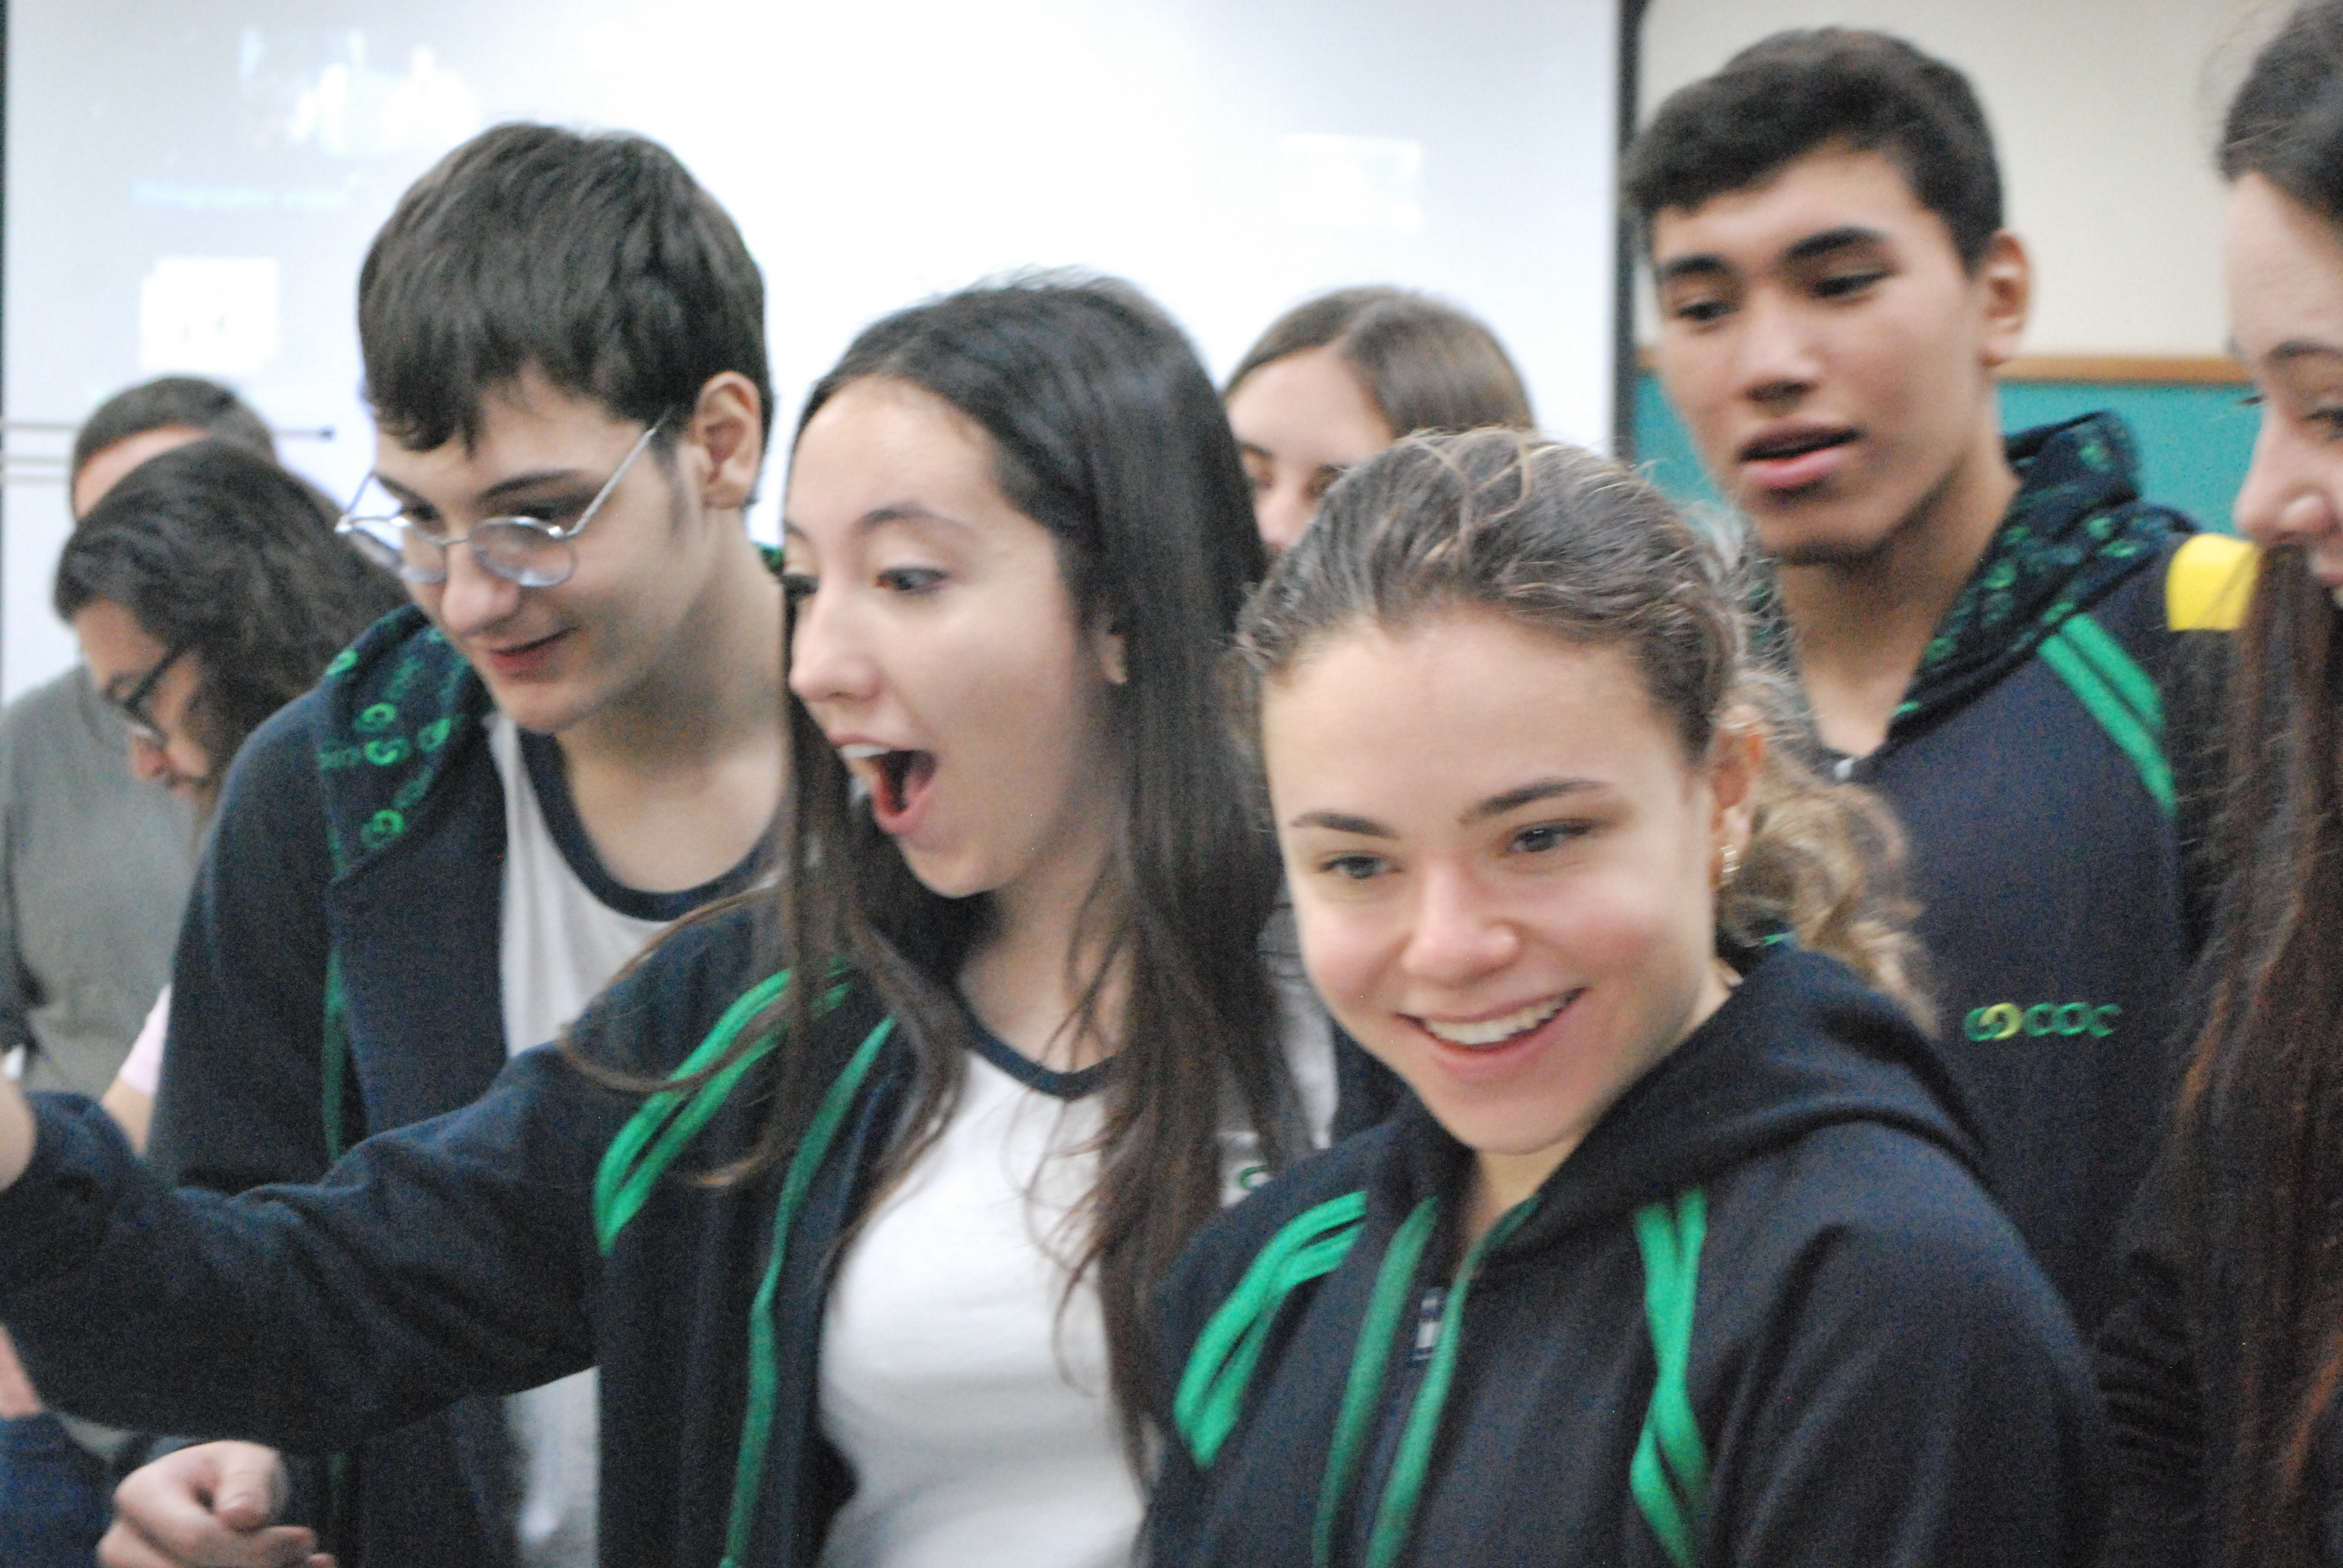
\includegraphics[width=0.7\linewidth,height=\textheight,keepaspectratio]{consideracoes/foto-espanto.jpg}

Que essa energia levada aos visitantes se mantenha viva até o próximo FT
de Portas Abertas.

Para finalizar, apresentamos a mensagem de Adolfo Pérez Esquivel (Prêmio
Nobel da Paz em 1980) sobre a importância da Educação, enviada
especialmente para o FT de Portas Abertas por meio do Prof.~Yuri Meyer.

\url{video-adolfo-perez.mp4}

\begin{tcolorbox}[enhanced jigsaw, leftrule=.75mm, toprule=.15mm, opacitybacktitle=0.6, bottomtitle=1mm, breakable, rightrule=.15mm, titlerule=0mm, colback=white, colbacktitle=quarto-callout-caution-color!10!white, title=\textcolor{quarto-callout-caution-color}{\faFire}\hspace{0.5em}{Adolfo Pérez Esquivel}, toptitle=1mm, arc=.35mm, left=2mm, opacityback=0, coltitle=black, bottomrule=.15mm, colframe=quarto-callout-caution-color-frame]

Adolfo Pérez Esquivel é um ativista argentino dos direitos humanos,
nascido em 26 de novembro de 1931, em Buenos Aires. Reconhecido por sua
atuação não violenta em defesa da justiça social e dos direitos dos
povos da América Latina, recebeu o Prêmio Nobel da Paz em 1980,
tornando-se um símbolo internacional da resistência pacífica contra
regimes autoritários. Fundador do Servicio Paz y Justicia (SERPAJ),
enfrentou a repressão militar durante as ditaduras do Cone Sul, sendo
preso e torturado por seu ativismo. Esquivel também é artista plástico,
escritor e educador, e continua sendo uma voz ativa em favor da paz, da
dignidade humana e da solidariedade entre os povos.

\end{tcolorbox}




\end{document}
